\documentclass[12pt]{article}
\usepackage{graphicx,rotating,hyperref}

\oddsidemargin  -0.5 cm
\evensidemargin 0.0 cm
\textwidth      6.5in
\headheight     0.0in
\topmargin      -1 cm
\textheight=9in

\newcommand{\s}[1]{{\mbox{\scriptsize #1}}}

\title{Oct 2010 Endcap Ring Alignment}
\author{Jim Pivarski}

\begin{document}
\maketitle
\tableofcontents

\section{Motivation}

The CSC ring positions currently used to reconstruct endcap muons are
derived from $p_T > 100$~GeV/$c$ cosmic rays, which have incomplete
information about the vertical positions of the rings due to the
paucity of horizontal cosmic ray tracks.  In addition, the method has
been made significantly more robust due to new studies presented in
this note.  It is therefore worthwhile to re-align the rings using
$\phi$-symmetric collisions data with the improved methods.

Two techniques will be described in this note: ring alignment relative
to the tracker using tracks from collisions and ring alignment
relative to one another, using the long ``straight-through'' beam-halo
tracks that cross three or four stations.  The first method is more
complete and will be used for the final alignment.  The second method
will be used as a cross-check.  Since the two methods use completely
disjoint sets of tracks, they are statistically independent, and since
the methods are so different, they share few systematic uncertainties.

\section{Ring alignment procedure with tracks from the tracker}
\label{sec:trackertorings}

To align CSC rings relative to the tracker, we propagate
tracker-tracks into the muon system and quantify the misalignment by
the pattern of differences between propagated muon trajectories and
observed muon hit positions (the residuals).  The tracker-to-muon
propagation was implemented by refitting GlobalMuon tracks with a
negligible weight applied to the muon hits (AlignmentPositionError =
$(\mbox{1000 cm})^2$), just like the Reference-Target algorithm.
Results of this method will be compared with results obtained with
re-reconstructed TrackerMuons, to check for any effect of the
refitted-GlobalMuon/TrackerMuon discrepancies observed in
Reference-Target studies on the bulk positions of rings.

If the rings are internally well-aligned (that is, if all chambers are
correctly aligned relative to one another within each ring), then the
expected pattern of residuals is a sine $+$ cosine $+$ constant curve
as a function of $\phi$.  The three constants from the fit are
directly related to the translational position (global $x$ and $y$)
and rotation angle around the beamline ($\phi_z$).  We apply these
corrections to the ring orientation, leaving the internal chamber
structure intact, and re-plot the residuals to confirm that our
interpretation was correct.  The final results are derived from two
successive applications of the procedure, to verify that the procedure
has reached self-consistency.

The explicit fit function of residuals versus $\phi$ is
\begin{equation}
\phi^g_z(\phi) = \delta_x R \sin\phi - \delta_y R \cos\phi - \delta_{\phi_z}
\label{eqn:fitfunc}
\end{equation}
\begin{itemize}
\item where $\phi^g_z$ is the ``$\phi$ residual,'' the difference between
the propagated track and muon segment in $\phi = \tan^{-1}(y/x)$;
\item $\phi$ is the position of the muon segment (not the muon track
  at the origin);
\item $R$ is the radius of the ring in question;
\item $\delta_x$, $\delta_y$, and $\delta_{\phi_z}$ are the explicit,
  global corrections to the geometry that make the system more aligned
  (with the above signs).
\end{itemize}

\subsection{Data samples}

The alignments presented here are based on almost 22~pb$^{-1}$ of
collisions data, rather than cosmic rays.  Collisions have the
advantage of $\phi$ symmetry, which is more important for
characterizing a $\phi$-trend than high statistics in any single bin.
Collisions have the disadvantage of having lower typical momentum than
cosmic rays.  A study of high- and low-momentum cosmic rays was
presented by Vadim at the Oct.~15 Muon Alignment
meeting\footnote{\url{http://indico.cern.ch/conferenceDisplay.py?confId=110638}}.

The data lumi-sections were selected using the latest official JSON
file from October 29, including runs 135821--144114 and 146428--148864
(CMS runs 2010A and part of 2010B).  The integrated luminosity is
3.1~pb$^{-1}$ (2010A) $+$ 18.8~pb$^{-1}$ (2010B) $=$ 21.9~pb$^{-1}$.
The explicit dataset names are
\begin{itemize}
\item \tt /Mu/Run2010A-MuAlCalIsolatedMu-Sep17ReReco\_v2/ALCARECO
\item \tt /Mu/Run2010B-MuAlCalIsolatedMu-v2/ALCARECO
\end{itemize}
for refittable GlobalMuons and
\begin{itemize}
\item \tt /Mu/Run2010A-Sep17ReReco\_v2/RECO
\item \tt /Mu/Run2010B-PromptReco-v2/RECO
\end{itemize}
for re-reconstructable TrackerMuons.  The Sep17ReReco and
2010B-PromptReco correspond to the same set of conditions (alignments
and calibrations).

In all cases, a $p_T > 15$~GeV/$c$ cut is applied to muons to avoid
the changing unprescaled trigger treshold (from 5 to 9~GeV/$c$ in
2010A to 11~GeV/$c$ in 2010B).

\subsection{Robust estimators and handling magnetic field errors}

Residuals are biased by several effects other than alignment, and
these must be properly accounted for.  The largest effects are
\begin{itemize}
\item non-multiple scattering, which gives rise to non-Gaussian tails
  in the residuals distribution;
\item material budget and magnetic field errors, which bias the
  residuals peak with equal magnitude in opposite directions for
  positively and negatively charged muons;
\item pion to muon decay-in-flight in which the pion and muon are
  incorrectly identified as a single track with a kink outside of the
  tracker volume.
\end{itemize}
The first two sources of systematic error are familiar from cosmic-ray
alignments, and we apply well-established techniques to minimize our
sensitivity to them.  The third source is unique to muons from
collisions.  We verify that decays-in-flight have negligible effect on
the ring placement through the cross-check with ``straight-through''
beam-halo muons, a sample which contains no decays-in-flight.

Figure~\ref{fig:residuals_peak_fit} illustrates the non-Gaussian tails
from non-multiple scattering and/or decays-in-flight.  In the
Reference-Target algorithm, these tails are controlled by modifying
the fit function to include a non-Gaussian component; here, we simply
perform a restricted Gaussian fit of the peak in multiple passes.  In
the first pass, residuals within $(-\mbox{RMS}, +\mbox{RMS})$ are
included in the fit; in a subsequent pass, residuals within $(-\sigma,
+\sigma)$ of the previous fit are included.

\begin{figure}
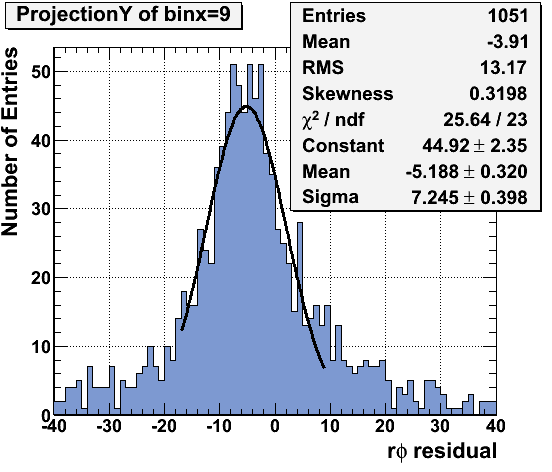
\includegraphics[height=6 cm]{residuals_peak_fit.png} \hfill
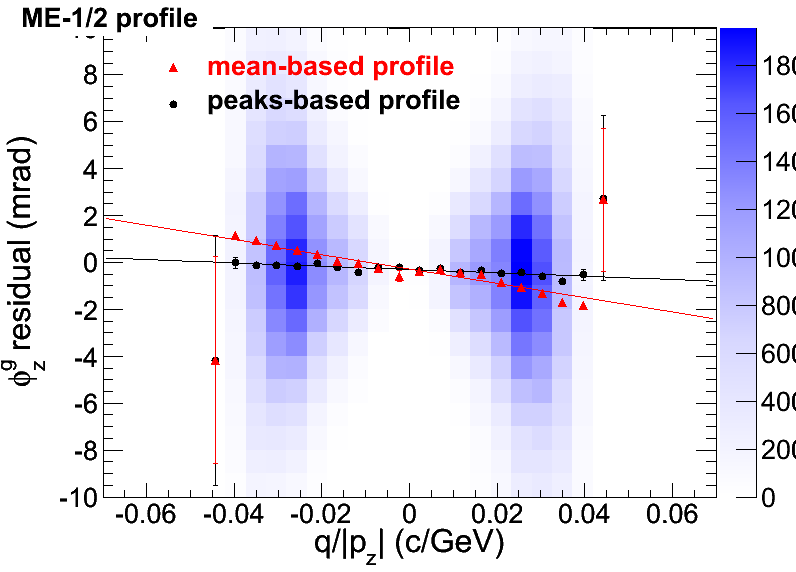
\includegraphics[height=6 cm]{residuals_qoverpz_fit.png}

\caption{Left: residuals histogram illustrating the large non-Gaussian
  tails and restricted Gaussian fit to identify the peak position.
  Right: residuals versus $q/|p_z|$ with points determined by the mean
  of vertical slices (red) and points determined by the restricted
  Gaussian peak-fits (black). \label{fig:residuals_peak_fit}}
\end{figure}

The non-Gaussian tails have a strong dependence on
charge-over-momentum, $q/p_T$ and $q/|p_z|$, also shown in
Fig.~\ref{fig:residuals_peak_fit}.  This is expected for scattering
but not for decays-in-flight, indicating that a significant fraction
of the tails are due to scattering.

{\bf Magnetic field errors: to be filled in later.}  {\it In the most
  up-to-date set of plots,} I (Jim) don't see conclusive evidence of
magnetic field errors: the difference between positive and negative
muons far from the beamline could just as easily be a material budget
error.  The distinction would be seen in the residuals versus $q/p_T$
(for axial magnetic field errors) and $q/|p_z|$ (for radial magnetic
field errors): if these are linear and primarily affect the peak of
the residuals, then they are consistent with being magnetic field
errors; if the effect is significantly larger for low-momentum muons
and especially affects the tails (which seems to be demonstrated by
Fig.~\ref{fig:residuals_peak_fit}-b), then they are more consistent
with material budget errors.  Ultimately, we won't be able to
precisely map the material or magnetic field with this technique
because there are more free parameters than observables (e.g.\ a
charge-dependent bias that grows with distance from the beamline might
be a constant radial magnetic field error and our hard $p_T$ cut or a
radially-varying axial magnetic field error), but we can cancel the
effect by extracting the charge-symmetric residuals bias. {\bf (end
  FIXME).}

To cancel the effect of any possible magnetic field error or material
budget error, we extract the charge-symmetric part of the residuals
bias.  Magnetic field and material budget errors bias residuals in
equal and opposite directions for positively and negatively charged
muons of the same momentum, a charge-antisymmetric effect.
Misalignments, on the other hand, are independent of the charge of the
muons that are used to probe them.  Thus, we can cleanly separate
the misalignments from all charge-antisymmetric effects with a
polynomial fit as a function versus $q/p_T$ or $q/|p_z|$; in practice,
the function is linear so only the intercept (charge-symmetric) and
slope (charge-antisymmetric) terms are relevant.  Alternatively, we
can plot the residuals peak separately for positively and negatively
charged muons to graphically depict the average and deviation.  Both
are shown in Fig.\ref{fig:charge_decomposition}.

\begin{figure}
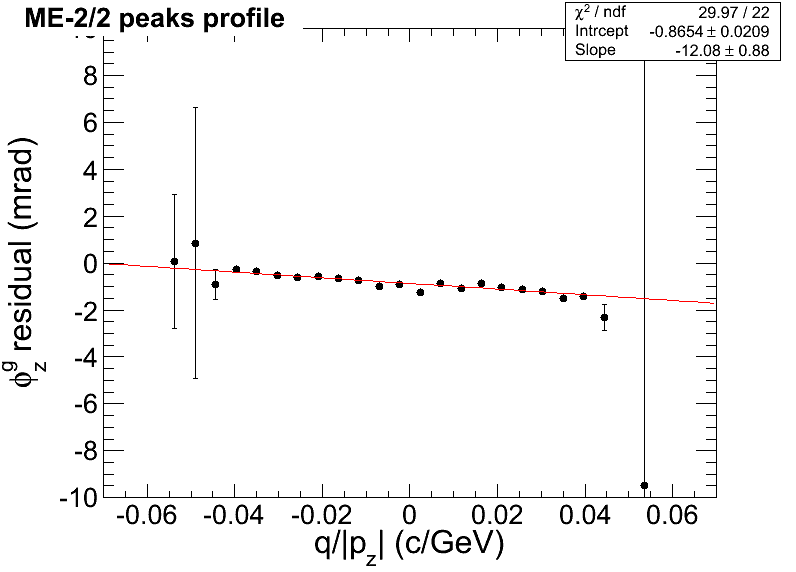
\includegraphics[height=6 cm]{charge_decomposition.png} \hfill
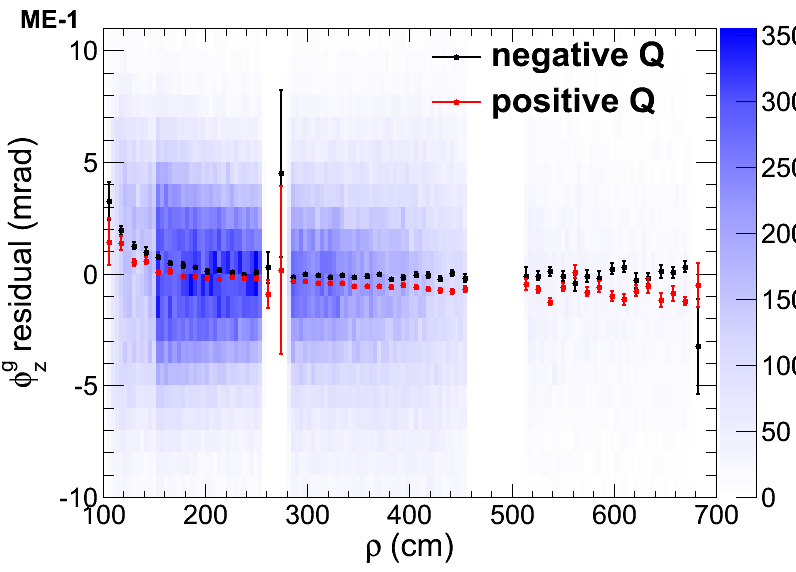
\includegraphics[height=6 cm]{charge_decomposition2.png}

\caption{Left: residuals versus $q/|p_z|$, indicating what might be a
  small radial magnetic field error (the slope), and a $-0.86$~mrad
  $\times$ $R$ misalignment (the intercept).  Right: residuals for
  positively and negatively charged muons as a function of distance
  from the beamline $\rho$. \label{fig:charge_decomposition}}
\end{figure}

With these corrections for robustness, the final procedure is the
following:
\begin{enumerate}
\item 1-$\sigma$ peak fit of $\phi^g_z$ residuals in $q/|p_z|$ and
  $\phi$ bins ($\phi$ of the segment, not the track at the origin);
\item linear fit of residuals-peaks versus $q/|p_z|$ in $\phi$ bins to
  determine the charge-symmetric part (the intercept);
\item plot the charge-symmetric part versus $\phi$, fit with
  Eqn.~\ref{eqn:fitfunc};
\item interpret the results of the fit as ring misalignments and
  correct the geometry;
\item repeat the whole procedure; the process converges within two
  iterations.
\end{enumerate}
ME$+$4/2, will be treated specially because it contains only five
chambers; it is not a $\phi$-symmetric ring.  Of the three fit
parameters in Eqn.~\ref{eqn:fitfunc}, only $\delta_{\phi_z}$ is
independently fitted for ME$+$4/2; $\delta_x$ and $\delta_y$ are
copied from ME$+$4/1.  In ME1/1, all corresponding ``a'' and ``b''
chambers are treated as single objects for collecting residuals and
applying alignment corrections.

\section{Tracker-to-ring alignment results}

A sample ``map-plot'' (residuals vs.\ $\phi$) is shown for ME$-$2/1 in
Fig.~\ref{fig:one_and_only_mapplot}, before any alignment (ideal ring
position).  {\bf FIXME: we need to see all of these, before and after
  alignment!}  Plots of residuals in the other projection, residuals
versus $\rho$, are shown in Fig.~\ref{fig:rphi_plots_vs_rho} after
ring alignment.  The special case of ME$+$4/2 is shown in
Fig.~\ref{fig:mapplot_me42} before alignment (ideal ring positions).
Tables and plots of the resulting corrections will be presented at the
end of this section, after describing how systematic uncertainties
were calculated.

\begin{figure}
\begin{center}
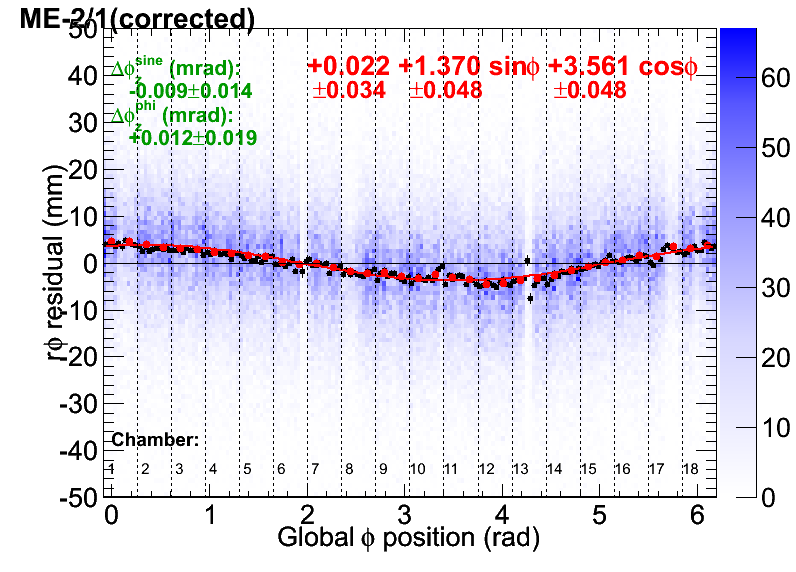
\includegraphics[height=6 cm]{one_and_only_mapplot.png}
\end{center}

\caption{Residuals versus $\phi$ for ME$-$2/1, where the residuals
  have been carefully fitted to determine the peaks and to cancel
  charge-antisymmetric biases.  The collisions data are
  $\phi$-symmetric and cleanly describe a single sinusoidal
  curve. \label{fig:one_and_only_mapplot}}
\end{figure}

\begin{figure}
\begin{center}
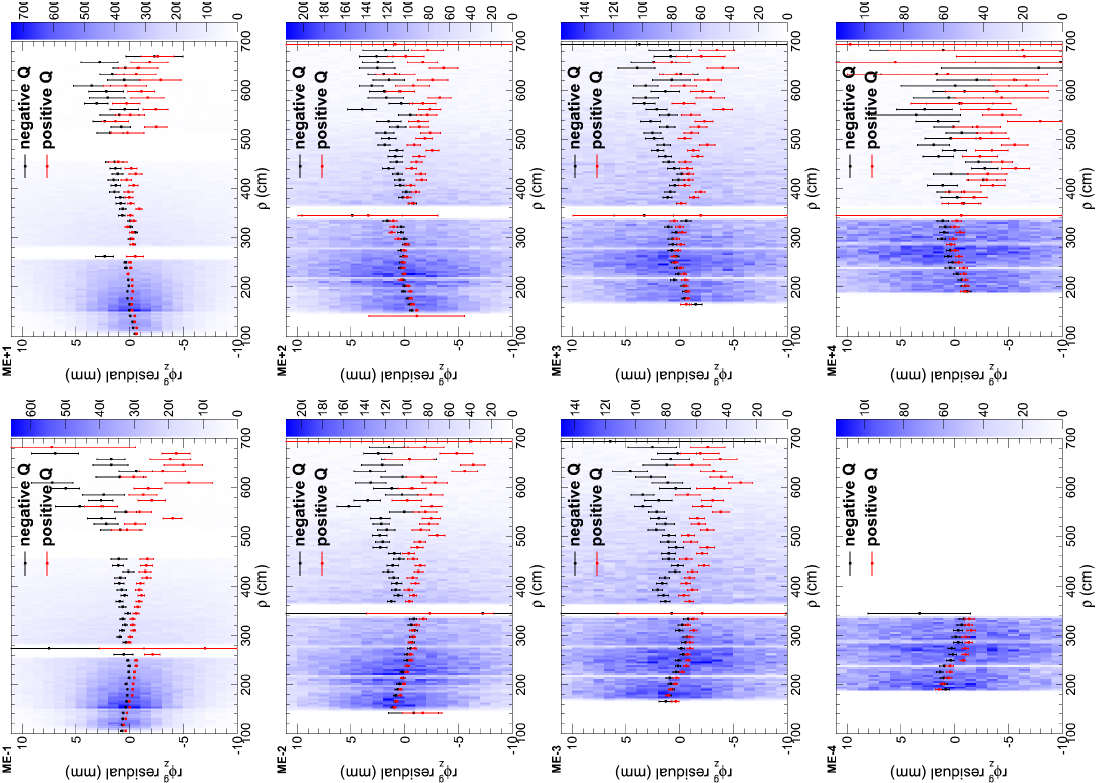
\includegraphics[height=0.85\linewidth, angle=-90]{rphi_plots_vs_rho.png}
\end{center}

\caption{Residuals ($r\phi$, in mm) versus distance from the beamline
  $\rho$ {\it after} ring-alignment.  There is a clear, consistent
  separation between positively and negatively charged muons that
  grows with $\rho$.  {\bf But is it magnetic field or material?  It
    would be interesting to see $q/p_T$ and $q/|p_z|$ in this region
    with proper momentum cuts (e.g.\ a $p_T$ cut over a range of $\rho$
    would cut a triangular region out of $q/|p_z|$ and bias the
    resulting picture).} \label{fig:rphi_plots_vs_rho}}
\end{figure}

\begin{figure}
\begin{center}
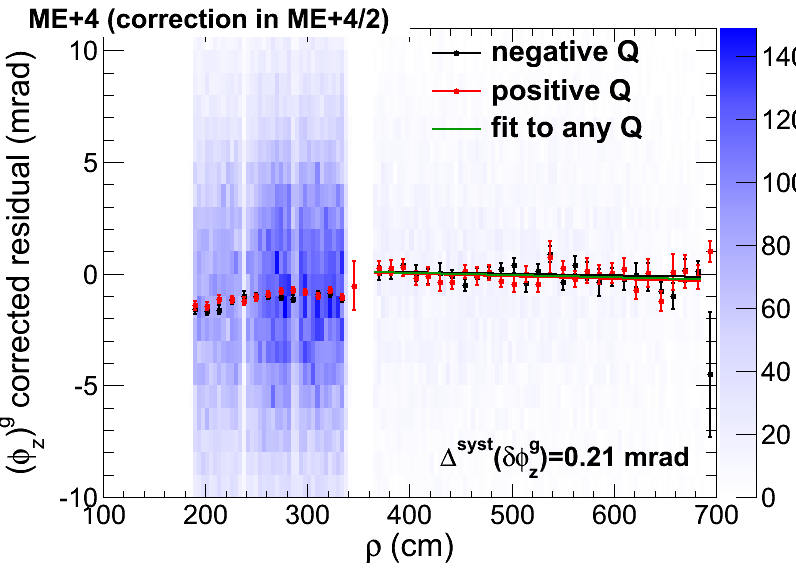
\includegraphics[height=6 cm]{mapplot_me42.png}  % not really a map-plot, sorry
\end{center}

\caption{Residuals versus $\rho$ in ME$+$4, showing the difference
  between ME$+$4/1 ($200 < \rho < 340$~cm) and ME$+$4/2 ($340 < \rho <
  700$~cm), before alignment.  A single-parameter ($\delta_{\phi_z}$)
  correction is made between the two rings. \label{fig:mapplot_me42}}
\end{figure}

\subsection{Study of systematic errors}
\label{sec:systematic_errors}

Two methods were used to quantify the systematic errors in the
alignment, both quantifying the deviations of the residuals
distribution from what would be expected for a single rigid ring.  One
quantifies the variation of the residuals in $\rho$, and the other
quantifies the variation in $\phi$.  The $\rho$ variation is the
dominant systematic uncertainty.

The $\rho$ systematic starts with the observation that even the
muon-antimuon average residual is not a constant with respect to
$\rho$.  This can be seen in Fig.~\ref{fig:rphi_plots_vs_rho}, but it
is highlighted for an extreme case (ME$-$1) in
Fig.~\ref{fig:vsmomentum_correction}.  This can be caused by coherent
$\phi_z$ misalignments in the internal alignment of the rings using
beam-halo along the chamber overlaps: the overlaps measurements are
only sensitive to {\it differences} in $\phi_z$ misalignment between
neighboring pairs of chambers, so a pure beam-halo alignment can only
result in all chambers having the same $\phi_z$ misalignment.  This is
mitigated by the fact that the internal alignments combine beam-halo
and photogrammetry data, which resolves this last degree of freedom.
However, the effect of any remaining $\phi_z$ rotation would be
amplified in this plot by the fact that all chambers have the same
rotation angle.  This internal misalignment makes the definition of a
correct ring alignment ambiguous: should we align the bottoms of the
chambers (edge closest to the beamline) or the tops?  Averaging all
residuals would yield a result that depends on the $\eta$ distribution
of the source.  Therefore, difference between the minimum and the
maximum is taken to be a systematic uncertainty.

\begin{figure}
\begin{center}
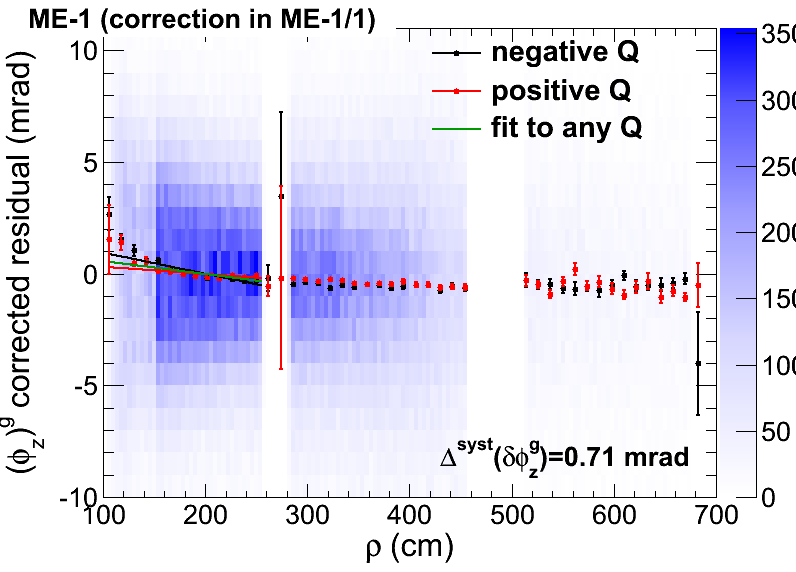
\includegraphics[height=6 cm]{vsmomentum_correction.png}
\end{center}

\caption{Residuals versus $\rho$ for ME$-$1, showing the linear slope
  in ME$-$1/1.  Either the $\rho=100$~cm edge or the $\rho=260$~cm
  edge could be aligned to zero, or something in between, so we take
  the difference in residuals between the two edges as a systematic
  uncertainty in the position of the ring. \label{fig:vsmomentum_correction}}
\end{figure}

The second systematic uncertainty allows for deformations in the
circularity of the ring, also due to possible internal misalignments.
Each ring is divided into four different half-ring subsets and
re-fitted with Eqn.~\ref{eqn:fitfunc}, as shown in
Fig.~\ref{fig:vsphi_systematic}.  Deviations in the $r\phi$ structure
of the ring from a perfect circle would result in different
$\delta_x$, $\delta_y$, $\delta_{\phi_z}$ solutions: differences from
the full-ring fit are taken as an additional systematic uncertainty.
The uncertainties from $\rho$ variations are much larger than the
uncertainties from these $\phi$ variations.

\begin{figure}
\begin{center}
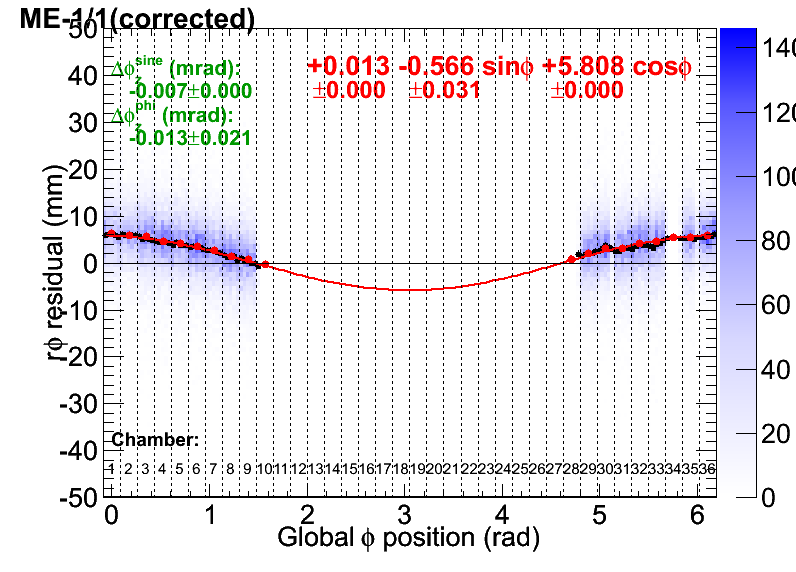
\includegraphics[width=0.45\linewidth]{vsphi_systematic1.png}
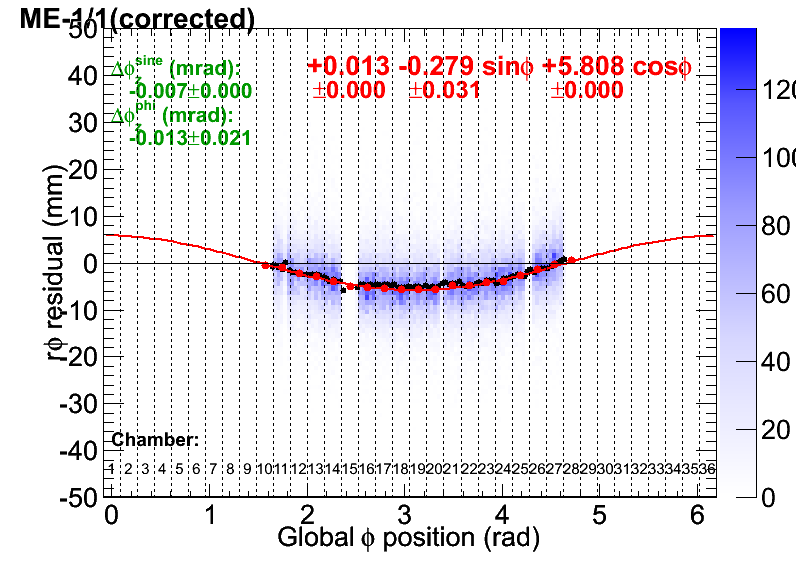
\includegraphics[width=0.45\linewidth]{vsphi_systematic2.png}

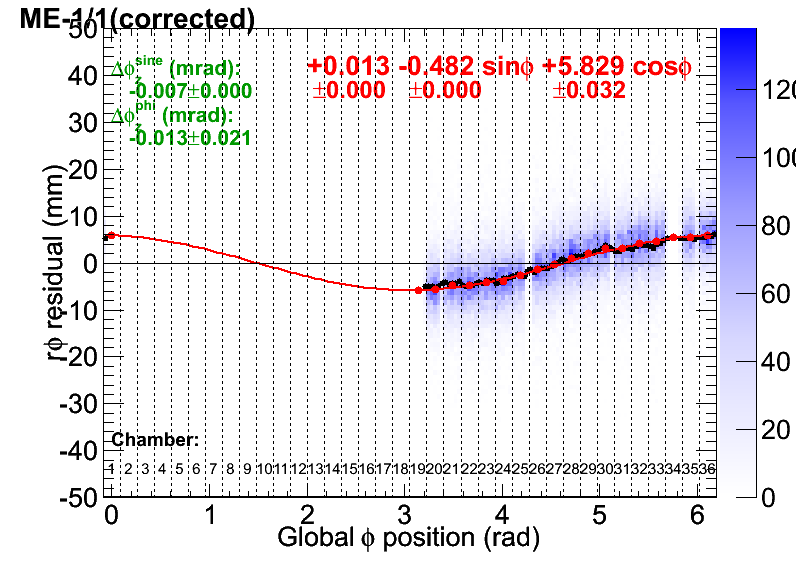
\includegraphics[width=0.45\linewidth]{vsphi_systematic3.png}
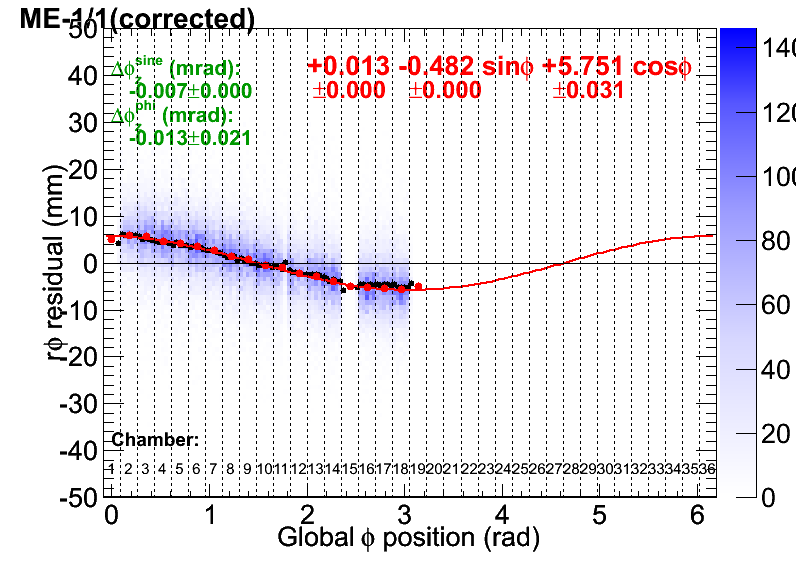
\includegraphics[width=0.45\linewidth]{vsphi_systematic4.png}
\end{center}

\caption{The ME$-$1/1 ring alignment determined by four different
  half-ring subsets.  If the residuals deviate from a sinusoidal curve
  due to internal misalignments, it would result in different
  $\delta_x$, $\delta_y$, $\delta_{\phi_z}$ solutions: this is taken
  as a second systematic uncertainty. \label{fig:vsphi_systematic}}
\end{figure}

\subsection{Tests for additional dependencies}
\label{sec:additional_tests}

The alignment of the previous section was tested in two additional
ways: by changing the internal ring geometry and by changing the
method used to calculate residuals.  Plots illustrating the results of
both will be shown in the next section.

Two internal alignments from beam-halo overlaps were delivered on
Oct.~29; in one fit, all photogrammetry constraints were applied
(``BHPG'' for beam-halo and photogrammetry) and in the other,
photogrammetry was only used to fill missing beam-halo data
(``BHPGholes'' for beam-halo with photogrametry ``filling the
holes'').  The decision on an optimal internal alignment method was
deferred until the completion of the ring-position alignment, to see
if a difference in residuals from the tracker could be observed.  Both
internal alignments yield smooth rings; they differ in final ring
alignment positions by 2~mm in ME$+$3/2 $\delta_y$, 0.5~mm in ME$-$3/2
$\delta_x$, all others are small (see Fig.~13 in the Oct.~29 HyperNews
paper; this is the same pattern as was seen in the internal plots,
though with a different magnitude).  Differences in the global offset
of the internal alignment is irrelevant because the global offset is
corrected by the ring-alignment procedure described in this note---
the only difference is in the pre-alignment initial condition.
Therefore, the choice between internal alignments is arbitrary, and I
would recommend the BHPGholes alignment, since it makes the
minimum-necessary use of photogrammetry.

Another important test is to check for differences between
refitted-GlobalMuons and re-reconstructed TrackerMuons in defining the
residuals.  The two methods ought to be equivalent, but differences
have been observed within individual chambers in the Reference-Target
alignment of the barrel.  These differences may be irrelevant in the
large-structure quantities $\delta_x$, $\delta_y$, and
$\delta_{\phi_z}$, so the ring-alignment was performed using both
methods, with final results compared in the next section.
Intermediate plots of residuals versus $\rho$ and $q/|p_z|$ are
presented in Fig.~\ref{fig:globalmuons_vs_trackermuons}.  Differences
in the final results are negligible compared to other systematic
uncertainties.

\begin{figure}
\begin{center}
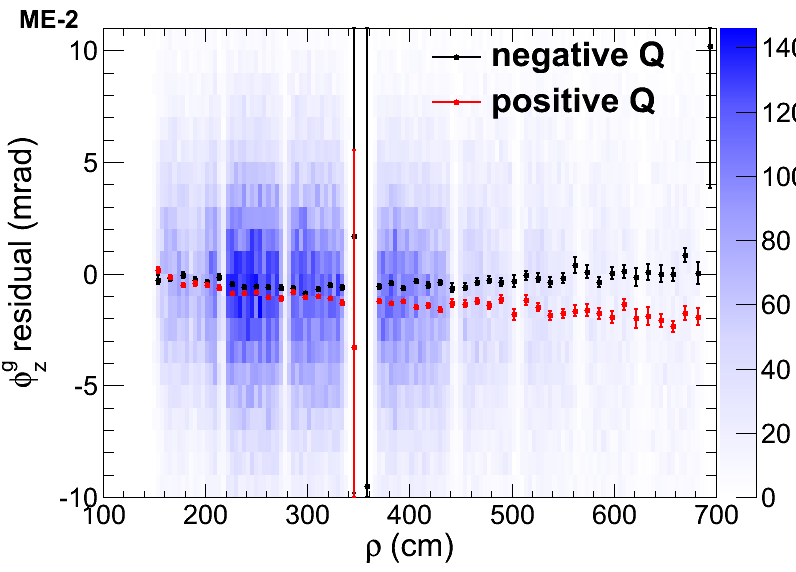
\includegraphics[height=3.5 cm]{globalmuons1.png}
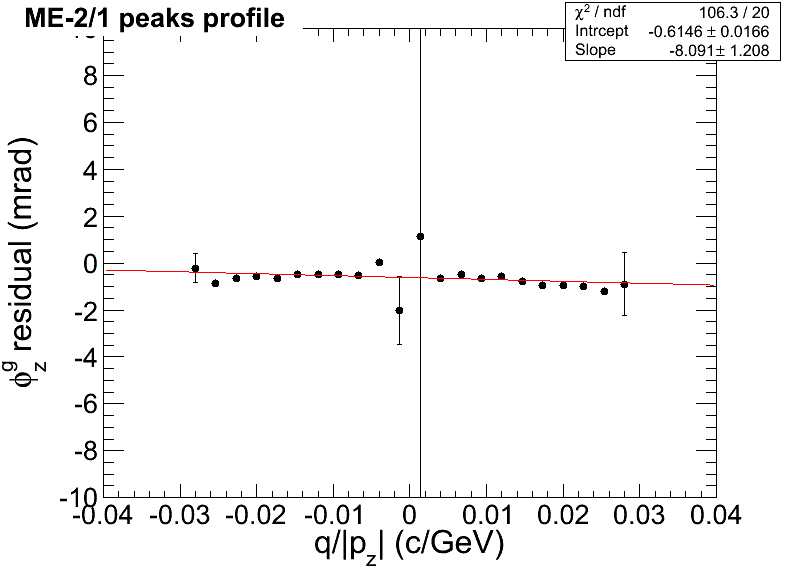
\includegraphics[height=3.5 cm]{globalmuons2.png}
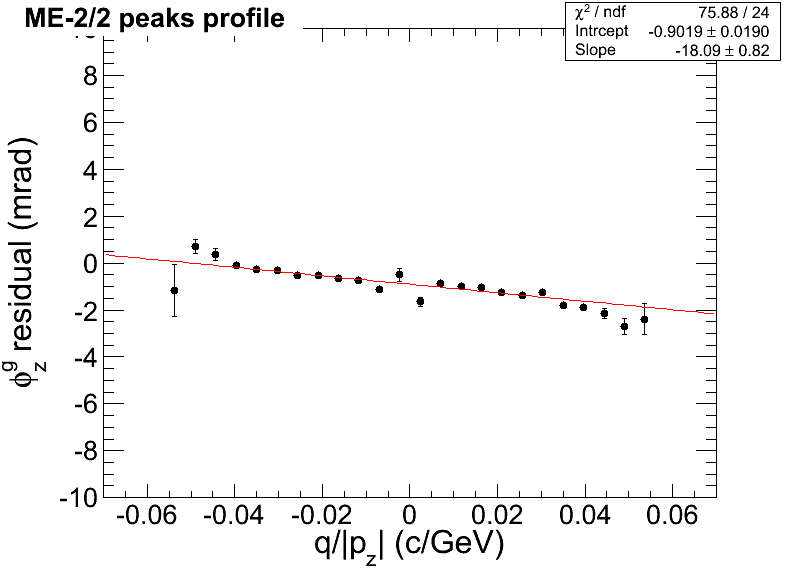
\includegraphics[height=3.5 cm]{globalmuons3.png}

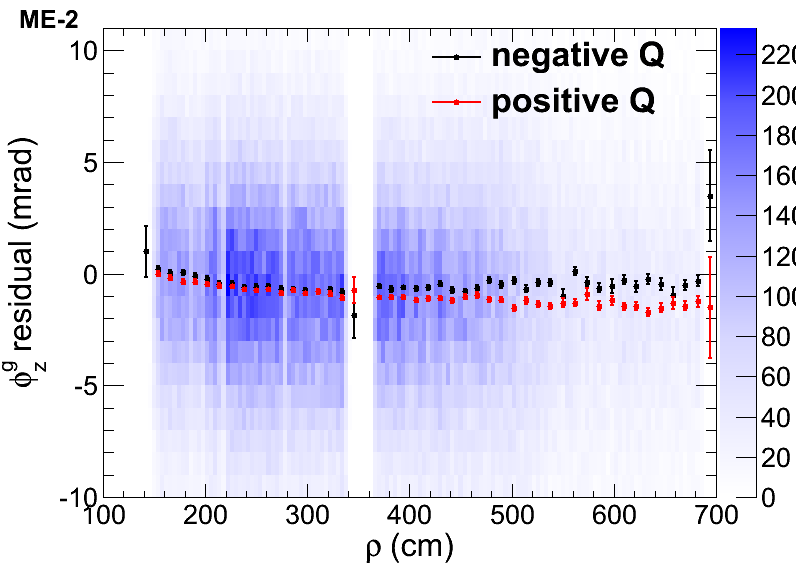
\includegraphics[height=3.5 cm]{trackermuons1.png}
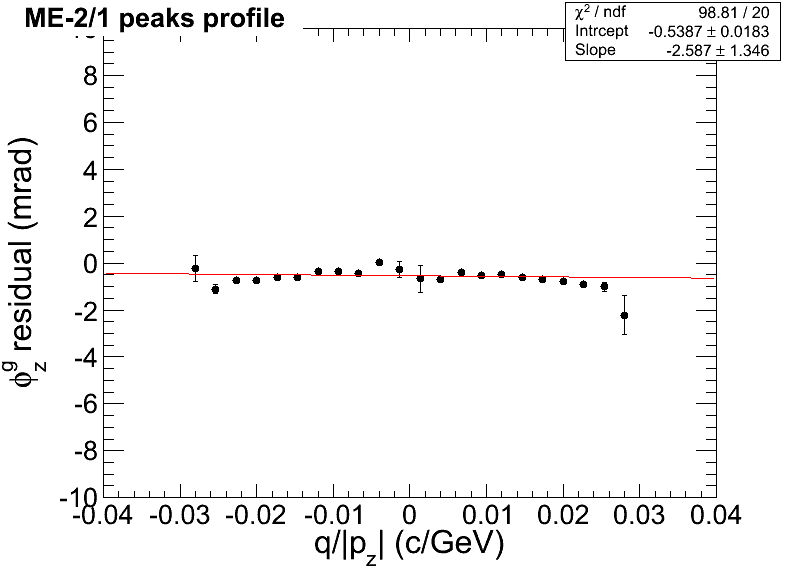
\includegraphics[height=3.5 cm]{trackermuons2.png}
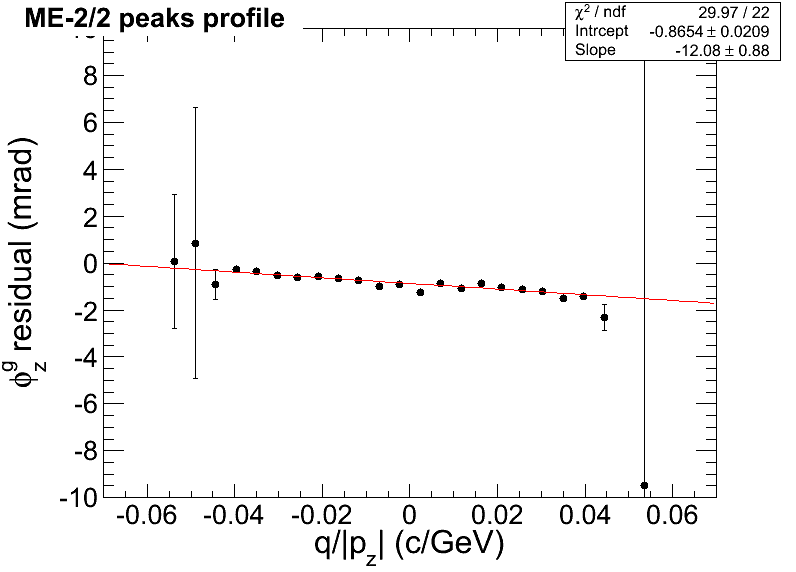
\includegraphics[height=3.5 cm]{trackermuons3.png}
\end{center}

\caption{Top row: residuals from refitted-GlobalMuons (versus $\rho$
  and $q/|p_z|$ for an inner and an outer ring).  Bottom row: same for
  re-reconstructed TrackerMuons.  The charge-splitting is slightly
  larger for GlobalMuons. \label{fig:globalmuons_vs_trackermuons}}
\end{figure}

\subsection{Final results}

Final results with systematic uncertainties are listed in
Table~\ref{tab:results}.  These results were computed using the
``beam-halo with photogrammetry only filling holes'' internal
alignment and re-reconstructed TrackerMuon residuals described in
Sec.~\ref{sec:additional_tests}.  They are not corrections relative to
what is currently in the database, but corrections relative to ideal
ring positions.  {\bf (Differences with respect to what is currently
  in the database are desirable, but not yet available.  To avoid
  interpretation errors from simply comparing this table to a table
  presented mid-summer, one should perform an alignment starting from
  the mid-summer geometry.  However, that geometry lacks important
  internal-ring alignment corrections.  The only rigorous comparison
  is at the level of individual chambers.)}  These values are plotted
in Figs.~\ref{fig:finalholes} and \ref{fig:finaltkgb} with
side-by-side comparisons of the two internal geometries and the two
methods of calculating residuals.  Corrections in the second iteration
are shown to be small in Fig.~\ref{fig:seconditer}, demonstrating that
the procedure has converged.

\begin{table}
\caption{Table of final ring-alignment corrections relative to
  ideal.  The first uncertainty is statistical (returned by the
  fitter) and the second is systematic, the sum of systematic error
  estimates from Sec.~\ref{sec:systematic_errors}. \label{tab:results}}
\begin{center}
\renewcommand{\arraystretch}{1.2}
\begin{tabular}{l c c c}
& $\delta_x$ (mm) & $\delta_y$ (mm) & $\delta_{\phi_z}$ (mrad) \\\hline
ME$+$4/2 & $+$0.86 $\pm$ 0.09 $\pm$ 0.61 & $+$5.33 $\pm$ 0.09 $\pm$ 0.67 & $-$1.28 $\pm$ 0.06 $\pm$ 0.21 \\
ME$+$4/1 & $+$0.86 $\pm$ 0.09 $\pm$ 0.61 & $+$5.33 $\pm$ 0.09 $\pm$ 0.67 & $-$0.27 $\pm$ 0.03 $\pm$ 0.39 \\
ME$+$3/2 & $-$0.16 $\pm$ 0.12 $\pm$ 1.85 & $-$0.94 $\pm$ 0.12 $\pm$ 2.50 & $-$0.09 $\pm$ 0.02 $\pm$ 0.27 \\
ME$+$3/1 & $+$0.03 $\pm$ 0.07 $\pm$ 0.30 & $+$0.15 $\pm$ 0.07 $\pm$ 0.51 & $+$0.28 $\pm$ 0.02 $\pm$ 0.31 \\
ME$+$2/2 & $+$0.57 $\pm$ 0.11 $\pm$ 1.46 & $+$0.59 $\pm$ 0.11 $\pm$ 1.69 & $+$0.06 $\pm$ 0.02 $\pm$ 0.27 \\
ME$+$2/1 & $+$0.31 $\pm$ 0.05 $\pm$ 0.32 & $-$0.24 $\pm$ 0.05 $\pm$ 0.39 & $+$0.32 $\pm$ 0.02 $\pm$ 0.42 \\
ME$+$1/3 & $+$4.35 $\pm$ 0.35 $\pm$ 0.57 & $+$3.37 $\pm$ 0.34 $\pm$ 0.10 & $-$0.00 $\pm$ 0.05 $\pm$ 0.15 \\
ME$+$1/2 & $+$3.56 $\pm$ 0.07 $\pm$ 1.31 & $+$1.71 $\pm$ 0.07 $\pm$ 1.94 & $+$0.21 $\pm$ 0.02 $\pm$ 0.27 \\
ME$+$1/1 & $+$4.30 $\pm$ 0.02 $\pm$ 0.46 & $-$2.10 $\pm$ 0.02 $\pm$ 0.40 & $+$0.03 $\pm$ 0.02 $\pm$ 0.57 \\\hline
ME$-$1/1 & $-$0.48 $\pm$ 0.02 $\pm$ 0.14 & $-$5.81 $\pm$ 0.02 $\pm$ 0.04 & $-$0.14 $\pm$ 0.02 $\pm$ 0.71 \\
ME$-$1/2 & $+$0.87 $\pm$ 0.06 $\pm$ 0.76 & $-$2.97 $\pm$ 0.06 $\pm$ 0.89 & $+$0.30 $\pm$ 0.02 $\pm$ 0.20 \\
ME$-$1/3 & $+$0.83 $\pm$ 0.33 $\pm$ 0.06 & $-$2.57 $\pm$ 0.37 $\pm$ 0.17 & $+$0.41 $\pm$ 0.04 $\pm$ 0.21 \\
ME$-$2/1 & $+$1.37 $\pm$ 0.05 $\pm$ 0.51 & $-$3.56 $\pm$ 0.05 $\pm$ 0.43 & $+$0.54 $\pm$ 0.02 $\pm$ 0.56 \\
ME$-$2/2 & $+$1.79 $\pm$ 0.11 $\pm$ 1.13 & $-$2.76 $\pm$ 0.11 $\pm$ 1.47 & $+$0.87 $\pm$ 0.02 $\pm$ 0.21 \\
ME$-$3/1 & $+$2.07 $\pm$ 0.07 $\pm$ 0.41 & $-$4.72 $\pm$ 0.07 $\pm$ 0.20 & $+$0.47 $\pm$ 0.02 $\pm$ 0.52 \\
ME$-$3/2 & $+$3.16 $\pm$ 0.12 $\pm$ 0.03 & $-$3.51 $\pm$ 0.12 $\pm$ 1.06 & $+$0.90 $\pm$ 0.02 $\pm$ 0.17 \\
ME$-$4/1 & $-$0.02 $\pm$ 0.09 $\pm$ 0.31 & $-$4.84 $\pm$ 0.09 $\pm$ 0.12 & $+$0.19 $\pm$ 0.03 $\pm$ 0.63 \\\hline
\end{tabular}
\end{center}
\end{table}

\begin{figure}
\begin{center}
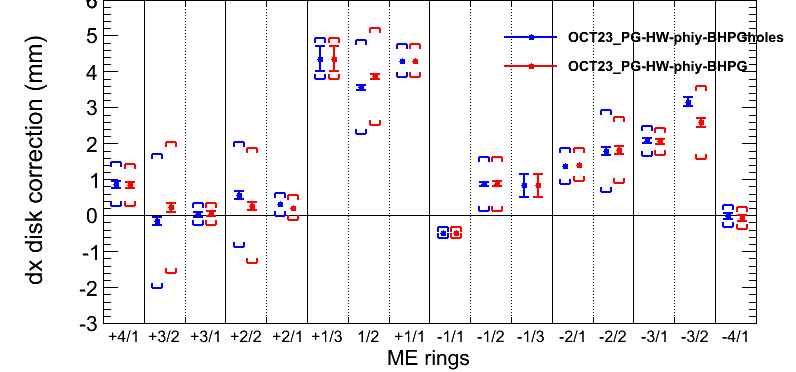
\includegraphics[width=0.85\linewidth]{finalholes1.png}

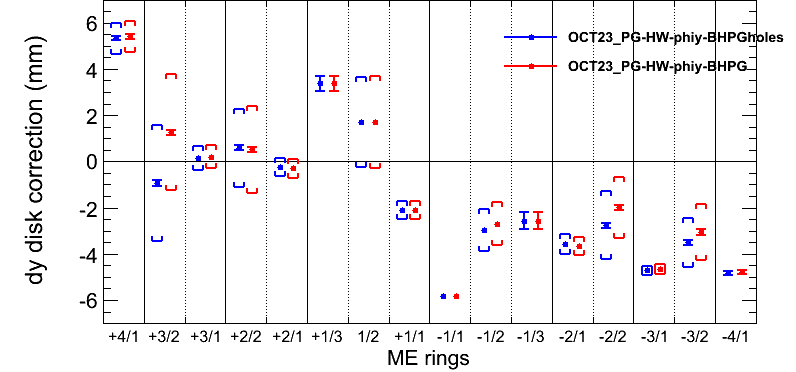
\includegraphics[width=0.85\linewidth]{finalholes2.png}

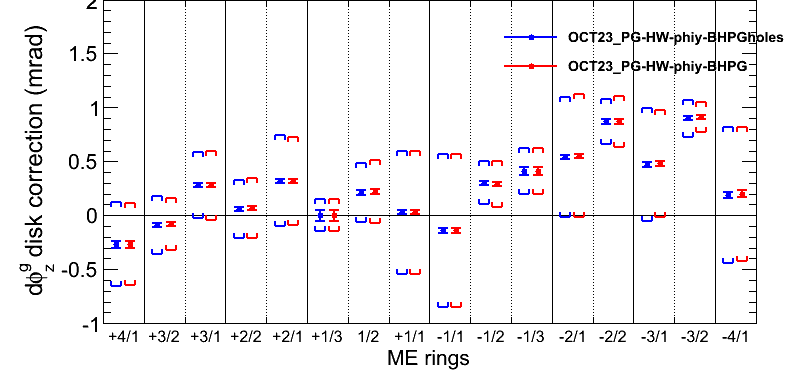
\includegraphics[width=0.85\linewidth]{finalholes3.png}
\end{center}

\caption{Final alignment quantities $\delta_x$ (top), $\delta_y$
  (middle), and $\delta_{\phi_z}$ (bottom) for all rings, computed
  using re-reconstructed TrackerMuons.  The error bars represent
  statistical and the brackets represent systematic uncertainties.
  The two colors indicate differences between results using the
  ``photogrammetry only filling holes'' internal alignment (BHPGholes,
  blue) and the ``all photogrammetry constraints'' internal alignment
  (BHPG, red); both described in
  Sec.~\ref{sec:additional_tests}. \label{fig:finalholes}}
\end{figure}

\begin{figure}
\begin{center}
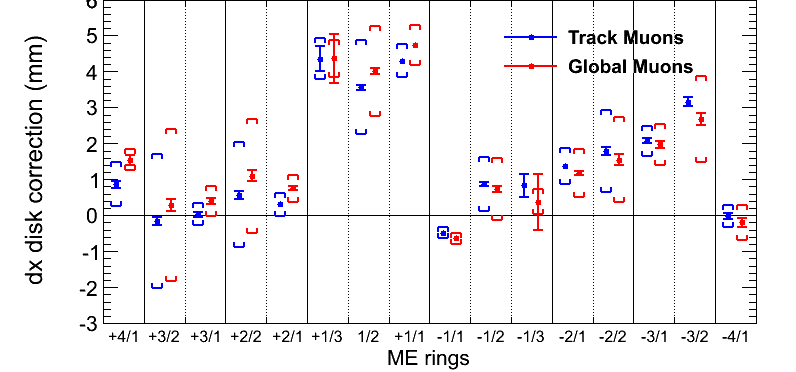
\includegraphics[width=0.85\linewidth]{finaltkgb1.png}

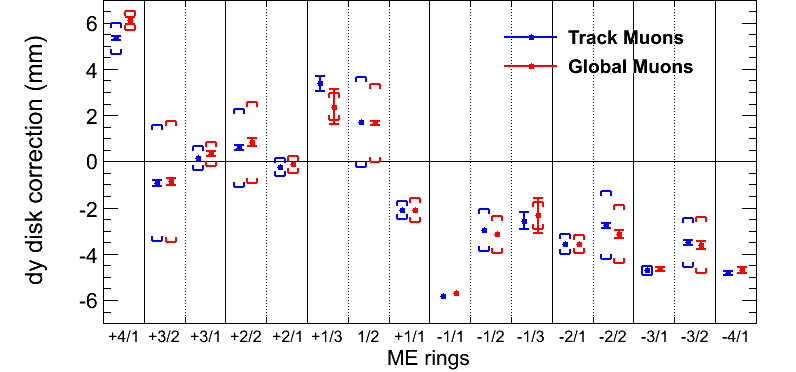
\includegraphics[width=0.85\linewidth]{finaltkgb2.png}

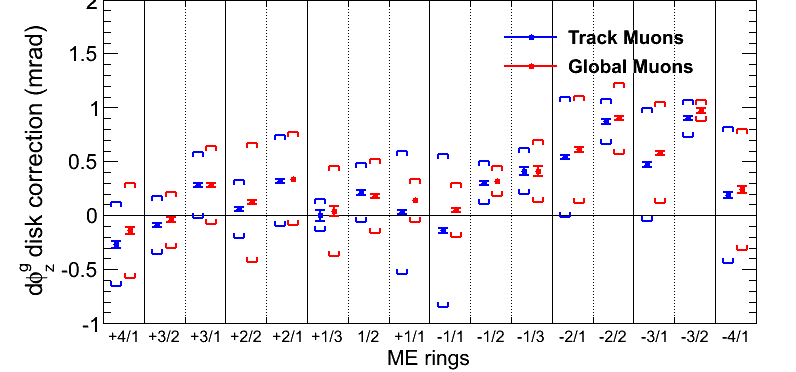
\includegraphics[width=0.85\linewidth]{finaltkgb3.png}
\end{center}

\caption{Final alignment quantities $\delta_x$ (top), $\delta_y$
  (middle), and $\delta_{\phi_z}$ (bottom) for all rings, computed
  using the ``photogrammetry only filling holes'' internal alignment.
  The error bars represent statistical and the brackets represent
  systematic uncertainties.  The two colors indicate differences
  between results using re-reconstructed TrackerMuons (blue) and
  refitted-GlobalMuons (red); both described in
  Sec.~\ref{sec:additional_tests}. \label{fig:finaltkgb}}
\end{figure}

\begin{figure}
\begin{center}
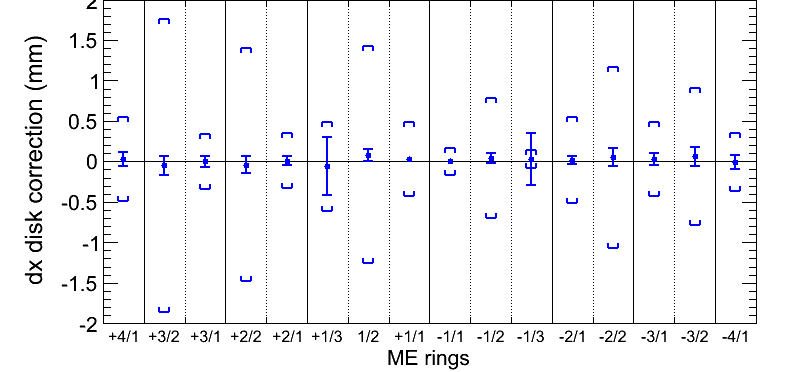
\includegraphics[width=0.85\linewidth]{seconditer1.png}

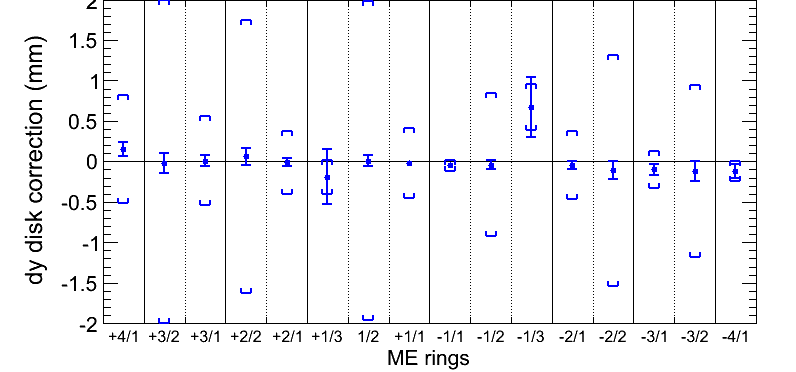
\includegraphics[width=0.85\linewidth]{seconditer2.png}

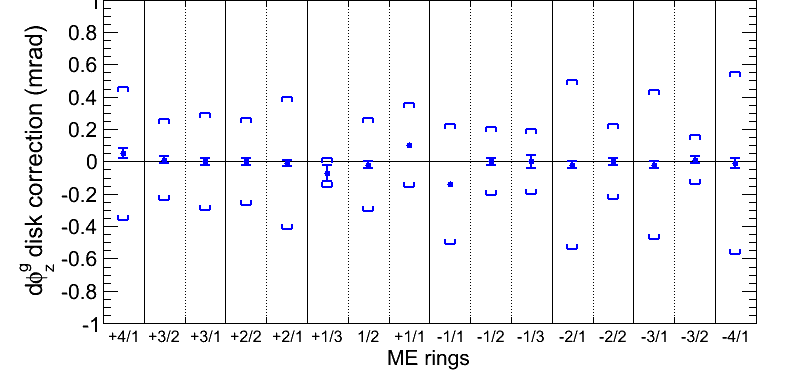
\includegraphics[width=0.85\linewidth]{seconditer3.png}
\end{center}

\caption{Changes in ring alignment parameters (top: $\delta_x$,
  middle: $\delta_y$, and bottom: $\delta_{\phi_z}$) in the second
  application of the procedure, demonstrating that the procedure has
  converged. \label{fig:seconditer}}
\end{figure}

\section{Cross-check with independent beam-halo muons}

Muons from collisions currently provide the best alignment of endcap
rings by aligning each ring relative to the tracker.  However, it is
also possible to align rings relative to one another using beam-halo
muons.  These muons are horizontal, do not cross the tracker, and
typically have higher momentum than muons from collisions (since they
originate in an LHC ``fixed target experiment'' with collimators
upstream of CMS).  The fact that these muons are parallel to the
largest component of the CMS magnetic field complicates the momentum
measurement, and the fact that they do not cross the tracker makes it
impossible to align them to that reference.  However, they provide a
nice cross-check of the standard ring alignment, since the
``absolute'' tracker-to-ring alignment method should automatically
yield a good ``relative'' ring-to-ring geometry.

Though both alignment procedures use tracks, they use disjoint sets of
tracks in very different ways.  No collisions muons are beam-halo
muons and vice-versa, a fact that is guaranteed by cuts on the polar
angles of the two samples: $|\eta| < 2.4$ for collisions and $|dr/dz|
< 0.12$ for beam-halo--- see Fig.~5 of the Oct.~29 HyperNews paper.
The differences in method are the following:
\begin{center}
\renewcommand{\arraystretch}{1.5}
\begin{tabular}{p{0.4\linewidth} c p{0.4\linewidth}}
Tracker-to-ring (collisions) & & Ring-to-ring (beam-halo) \\
$\bullet$ track parameters determined by tracker; & & $\bullet$ ``track parameters'' determined by one segment; \\
$\bullet$ full propagation through CMS magnetic field and material; & & $\bullet$ linear extrapolation from one station to the next; \\
$\bullet$ correction for magnetic field material errors with a $q/|p_z|$ fit; & & $\bullet$ correction for assuming zero field with an average of $\mu^+$ and $\mu^-$ results; \\
$\bullet$ best results close to the tracker, where the propagation is shortest. & & $\bullet$ best results far from the tracker, where the magnetic field is weakest.
\end{tabular}
\end{center}
Thus, the beam-halo alignment makes a nice cross-check on the
collisions alignment, particularly in ME4/1, where the tracker-tracks
have been propagated the farthest and the beam-halo tracks are
minimally affected by magnetic fields.

\subsection{Quantifying magnetic field for beam-halo tracks}

The velocity vector of beam-halo tracks is parallel to the axial
magnetic field, so they are not affected by the magnetic field
in the way that was designed for momentum measurement.  However, in the
CMS endcap, the radial magnetic field is strong enough to perform a
rough estimate of beam-halo momentum, useful for rejecting
low-momentum muons, which have wide residuals distributions.  To
construct an estimator independent of the ring positions themselves
and avoid a circular dependency, we compute the momentum from changes
in muon direction only, not position.  (In the tracker-to-ring method,
this independence derives from the fact that the momentum-measuring
detector, the tracker, is distinct from the detector being aligned,
the muon system.)  Changes in a track's $d\phi/dz$ entrance angle are
observed in three or four muon stations from the directions of the
muon segments.  The charge-times-momentum is
\begin{equation}
q \times p_z = \frac{B_r}{330~\mbox{ cm T/GeV}} \, \left(d\phi/dz\right)^{-1}.
\label{eqn:momentum}
\end{equation}
With this definition of momentum, note that we cannot distinguish
muons travelling in the $+z$ direction from antimuons travelling in
the $-z$ direction.  Without a known origin for the muons (such as the
beamspot), the two cases can only be distinguished by energy less in
material, which we are not including in this simple calculation.
However, most muons observed in the plus endcap are travelling in the
$-z$ direction and most muons observed in the minus endcap are
travelling in the $+z$ direction because CMS (in the lateral
direction) is a powerful attenuator for muons.

Figure~\ref{fig:momentum} presents Monte Carlo studies of this
momentum estimator for the three-station case (ME1--3) and the
four-station case (additionally including ME4/1).  Though the momentum
resolution is poor, an estimated-$p_z$ cut of 50~GeV/$c$ is sufficient
for eliminating muons with less than a few tens of GeV/$c$.
Figure~\ref{fig:qpz_spectrum} shows the distribution of real beam-halo
momentum, as determined by the three-station estimator.

\begin{figure}
\begin{center}
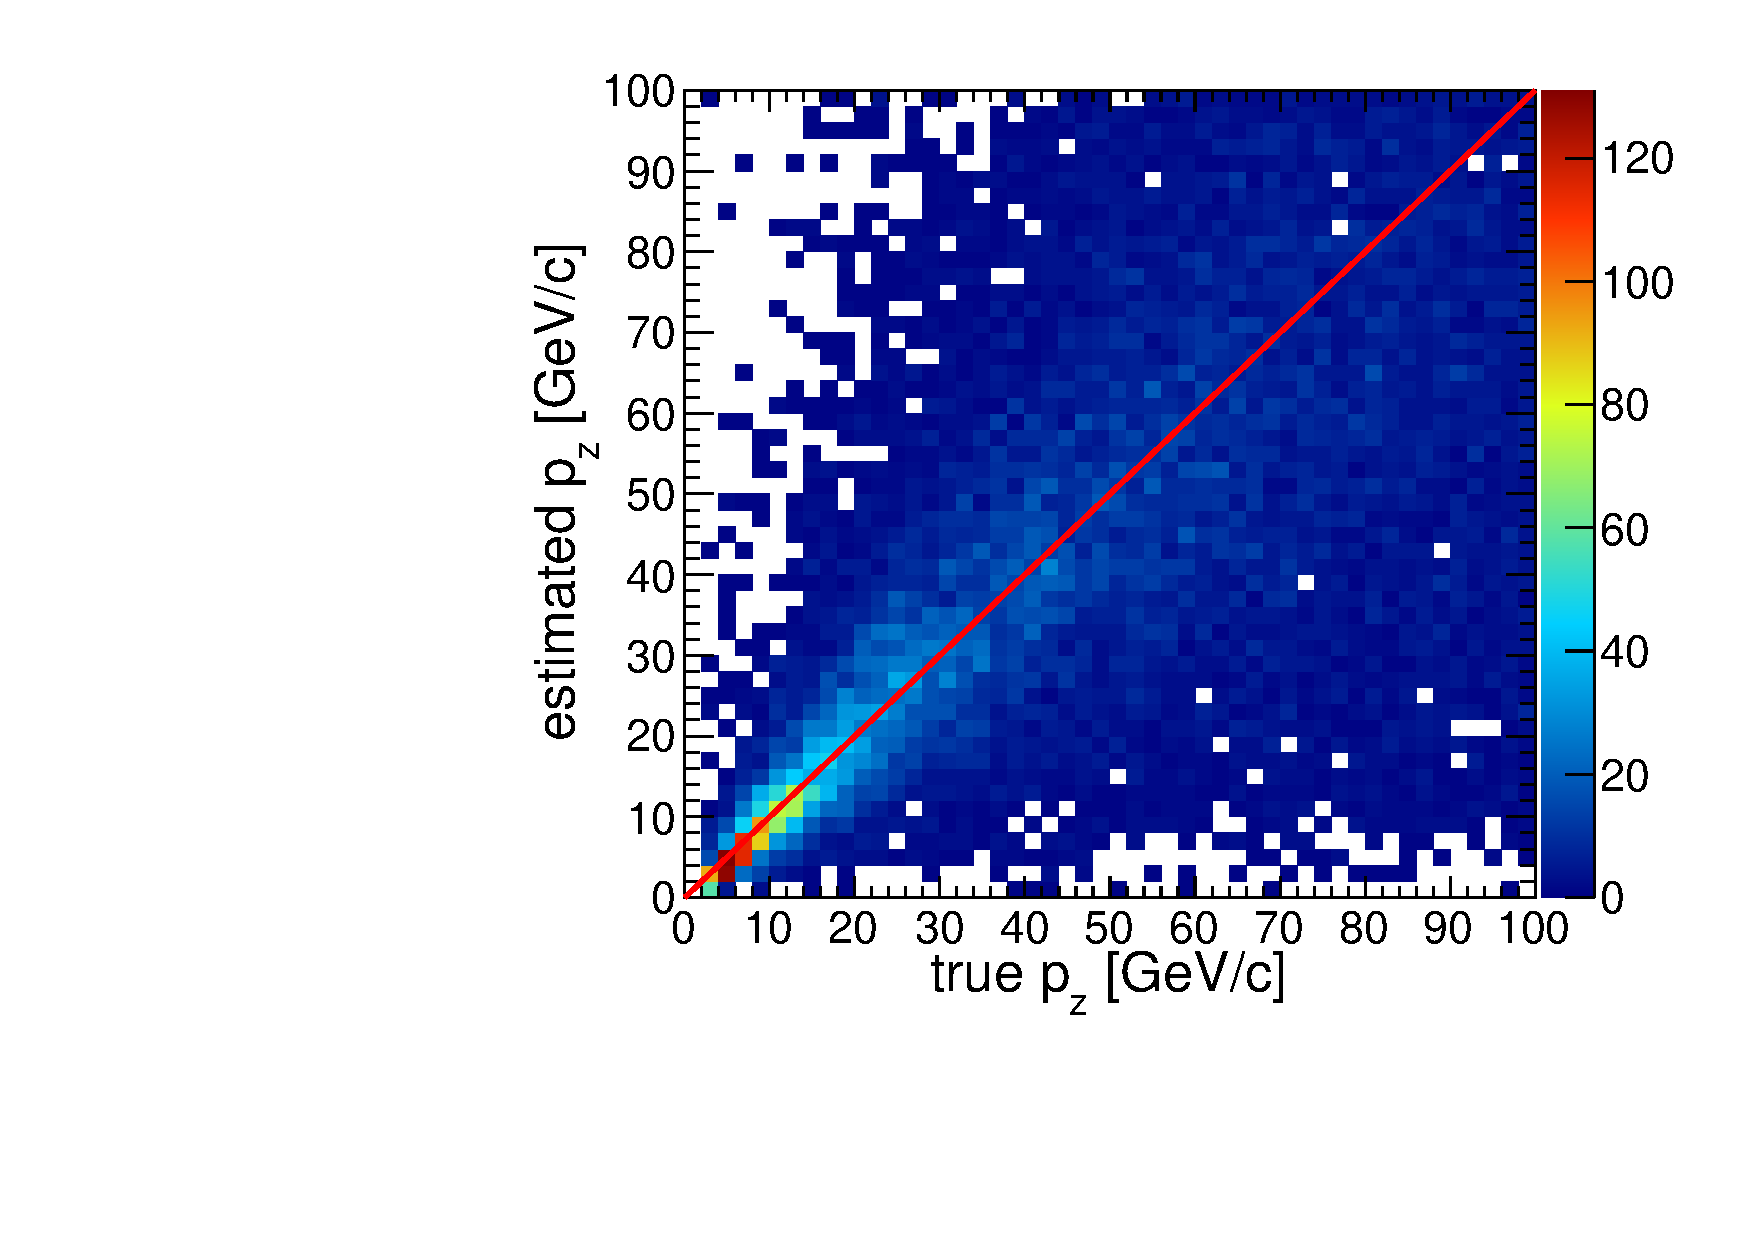
\includegraphics[width=0.4\linewidth]{estimator123_resolution.pdf}
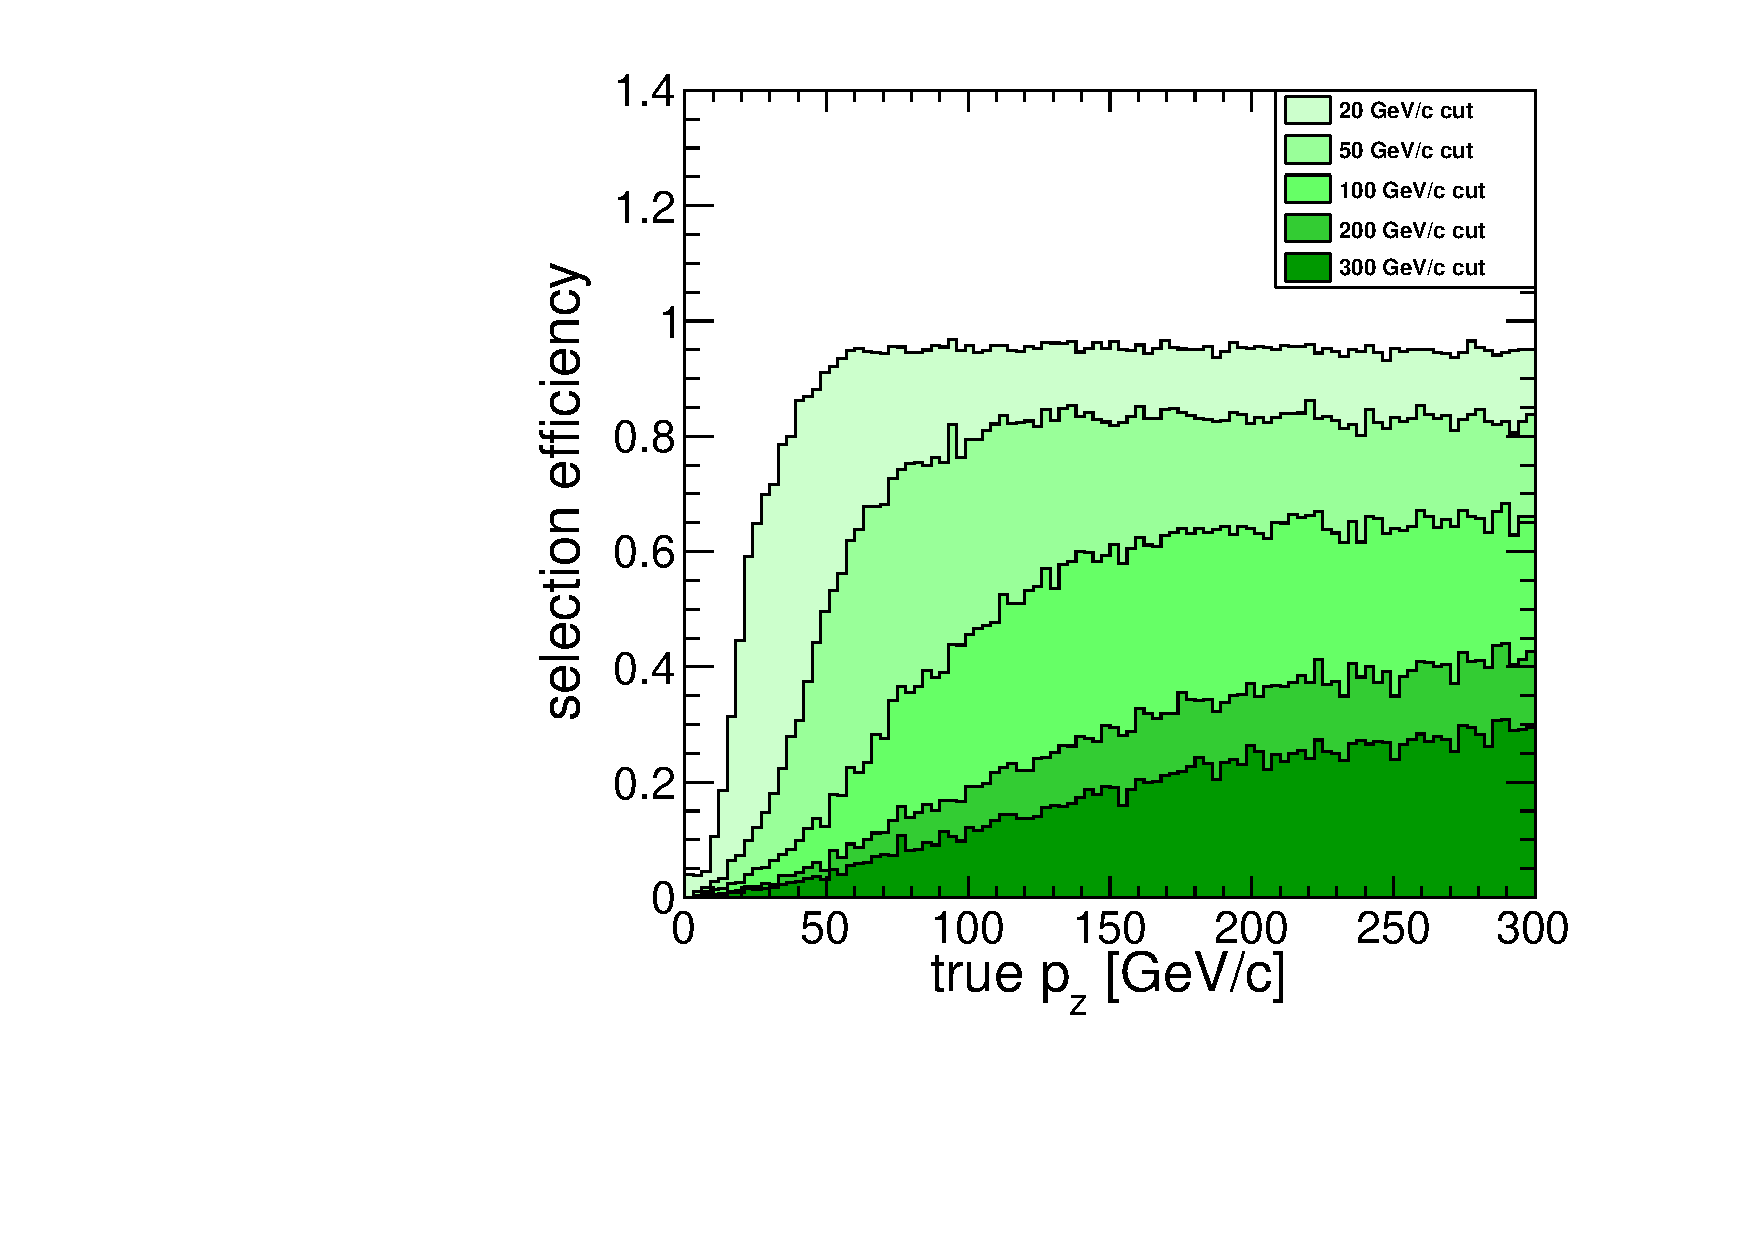
\includegraphics[width=0.4\linewidth]{estimator123_turnon.pdf}

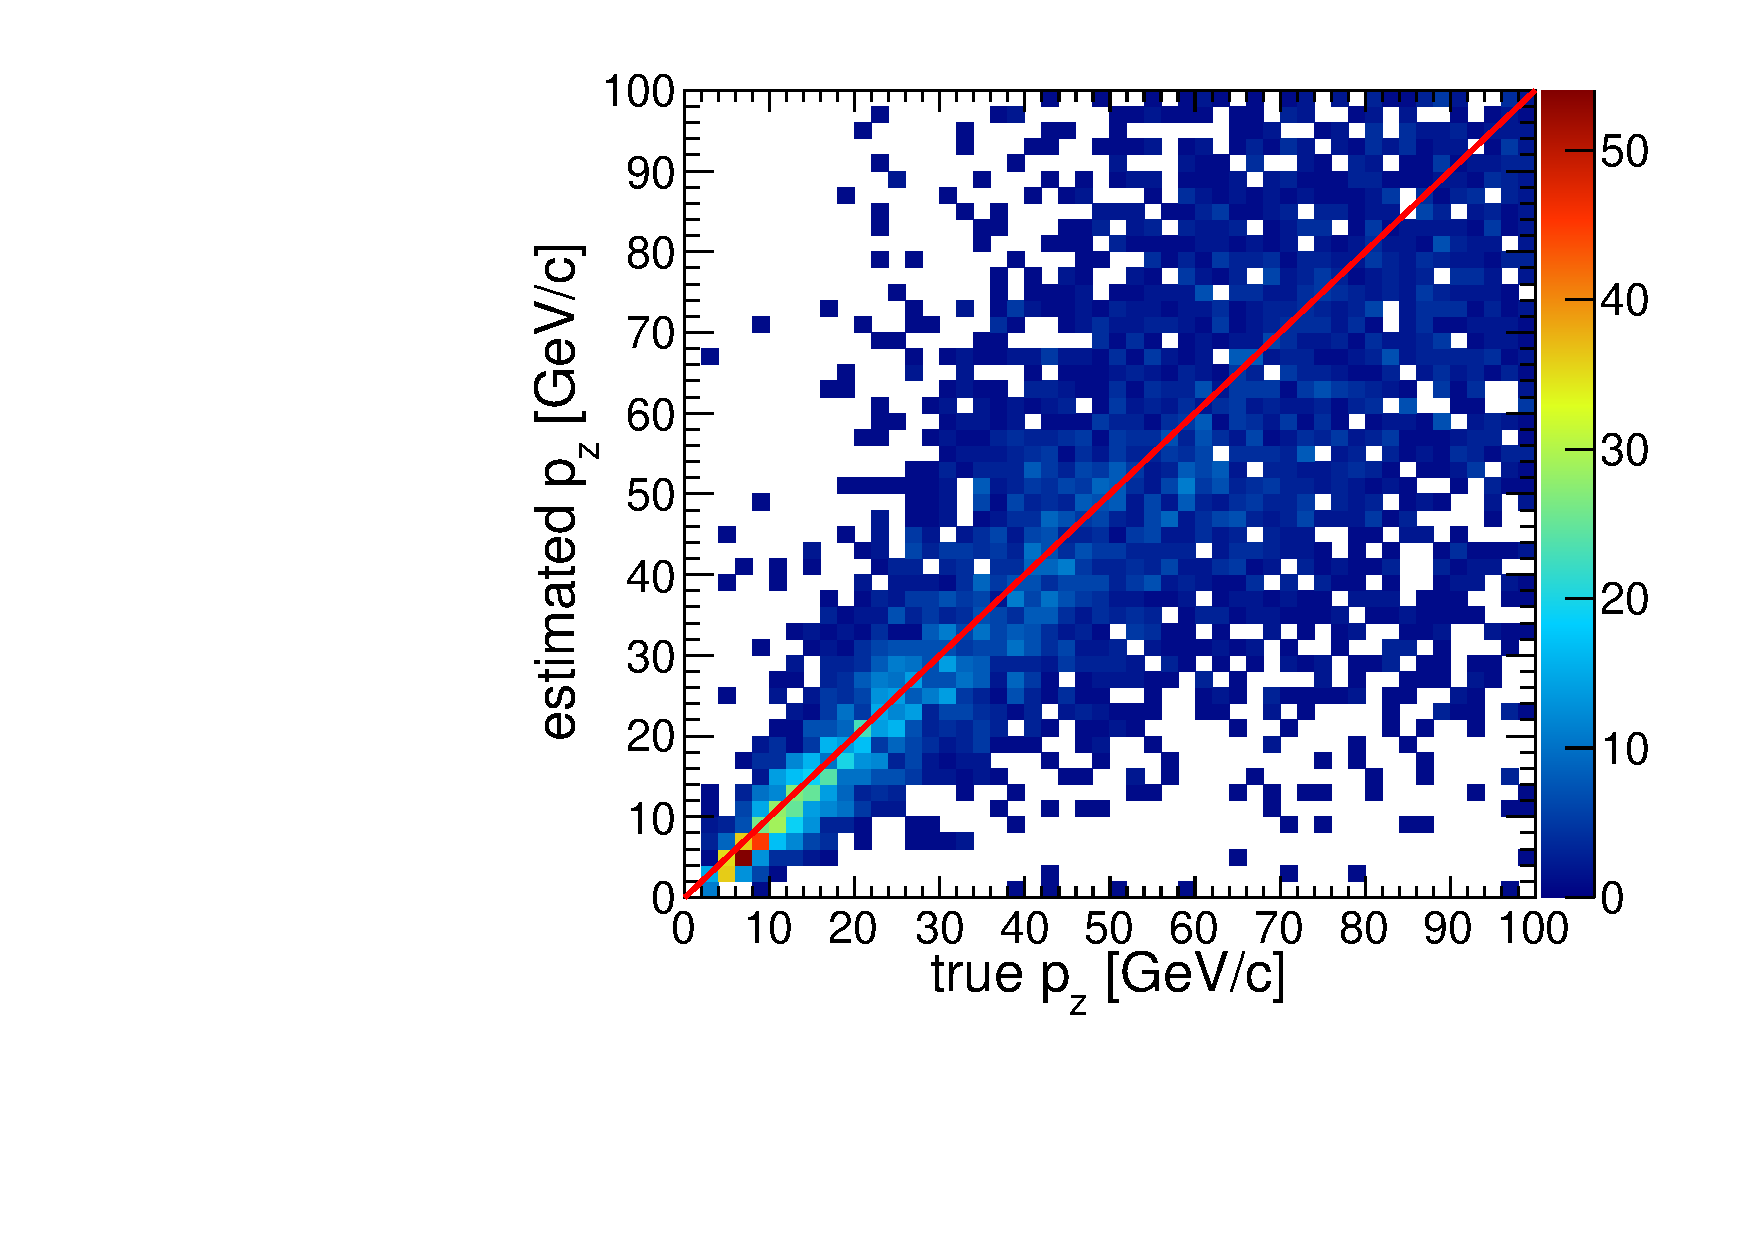
\includegraphics[width=0.4\linewidth]{estimator1234_resolution.pdf}
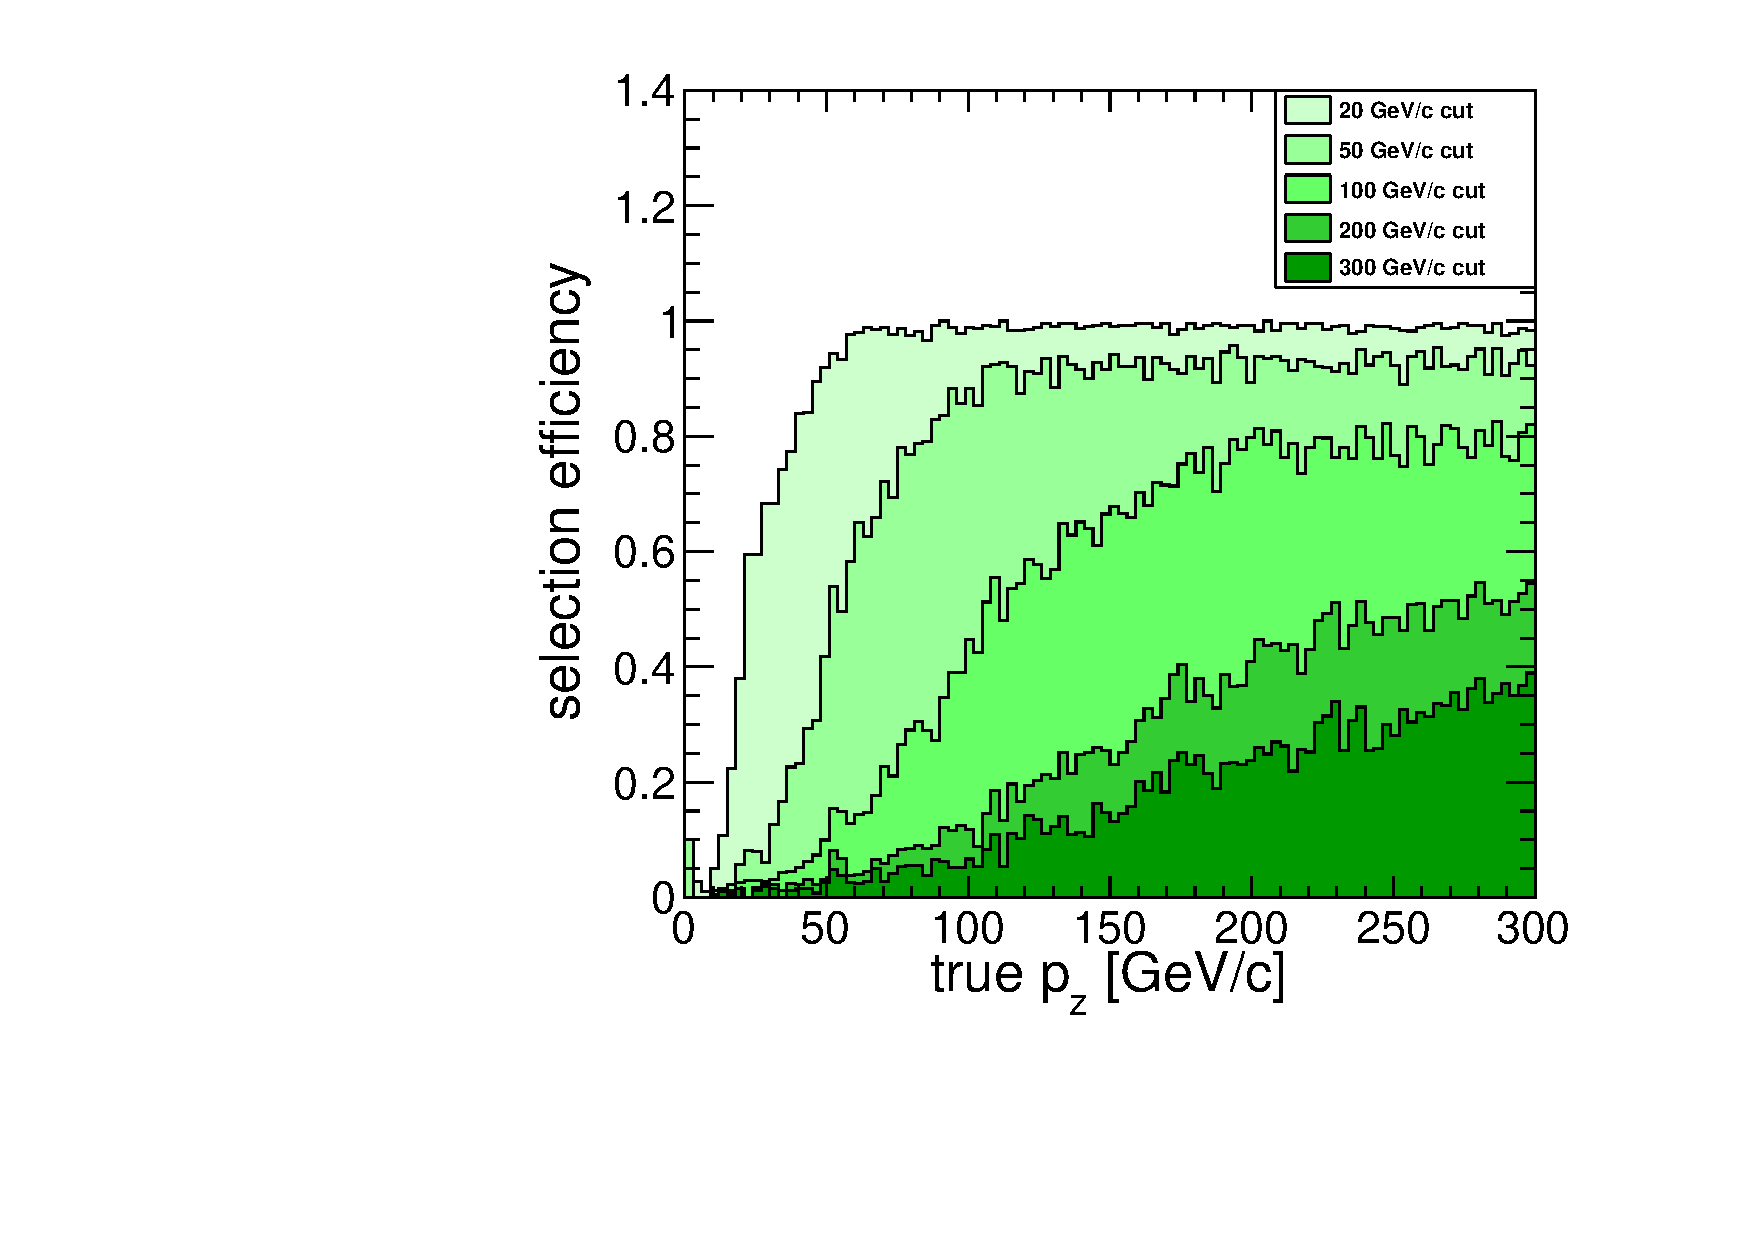
\includegraphics[width=0.4\linewidth]{estimator1234_turnon.pdf}
\end{center}

\caption{Momentum estimators of beam-halo muons studied in Monte
  Carlo; top: three-station estimator (ME1--3), bottom: four-station
  estimator.  Left: estimated $p_z$ compared to true $p_z$.  Right:
  efficiency versus true $p_z$ for various estimator-$p_z$ cuts.  In
  this analysis, we required a three-station $p_z > 50$~GeV/$c$ cut
  when studying relative alignments of ME1--3 and a four-station $p_z
  > 50$~GeV/$c$ cut when studying the alignment of ME4/1 relative to
  ME3/1. \label{fig:momentum}}
\end{figure}

\begin{figure}
\begin{center}
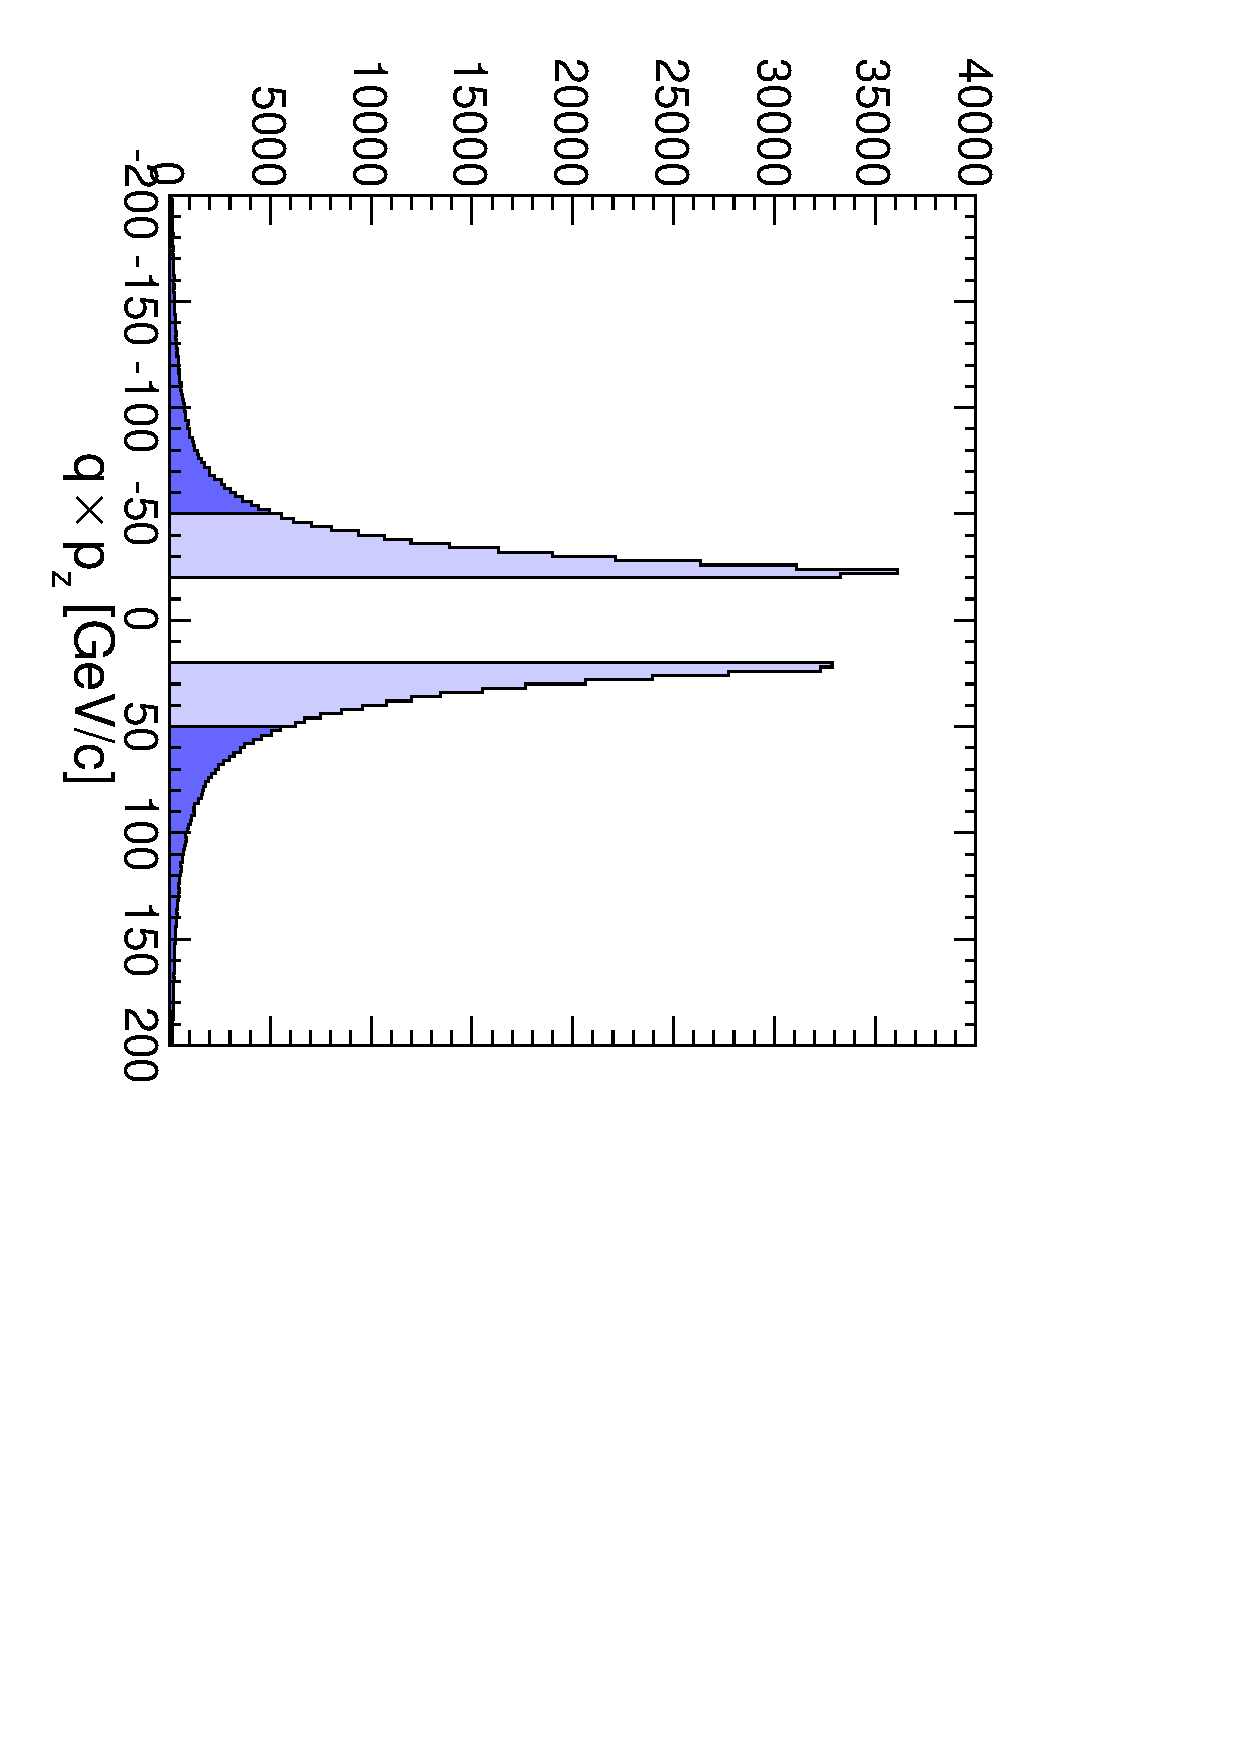
\includegraphics[height=0.4\linewidth, angle=90]{qpz_spectrum.pdf}
\end{center}

\caption{Momentum distribution of real beam-halo data with cuts at 20
  and 50~GeV/$c$ (three-station estimator). \label{fig:qpz_spectrum}}
\end{figure}

\subsection{Relative alignment datasets and method}

The dataset used here was derived from a special trigger and AlCaReco
stream to collect beam-halo muons during collisions.  It includes data
from mid-June (when single-beam intensities became sufficiently large)
until Sep.~1 (when the trigger was retired).  The AlCaReco stream is
{\tt /Cosmics/Run2010A-MuAlBeamHalo-v4/ALCARECO}.  We applied a $|p_z|
> 50$~GeV/$c$ cut to all cosmic-reconstructed muons in this sample and
computed alignment quantities from segments within these tracks.

To quantify the alignment of one ring relative to its neighbor,
segments in the reference ring were linearly extrapolated to the next
ring.  The difference in $r\phi$ position between the extrapolated
reference and the observed segment is defined as the $r\phi$ residual.
Peaks in the residuals distribution are fitted with restricted
Gaussians, much like the tracker-to-ring procedure.  The fact that the
segement extrapolation ignores magnetic fields is compensated for by
performing peak-fits independently for positively and negatively
charged muons and averaging the results.  (Positive and negative muons
are approximately identified by the sign of the $q\times p_z$
estimate.)  This procedure also relies sensitively on the $\phi_y$
alignment of chambers, which is derived from about 3~pb$^{-1}$ of
collisions TrackerMuons (see Jim's talk at the Oct.~8 Muon Alignment
meeting\footnote{\url{http://indico.cern.ch/conferenceDisplay.py?confId=109787}}).
The resulting residuals biases in bins of $\phi$ are fitted to
Eqn.~\ref{eqn:fitfunc} before and after the tracker-to-ring alignment.

\subsection{Cross-check results}

Beam-halo residuals are presented in $r\phi$ residual versus $\phi$
plots for all relevant pairs of rings.
Figure~\ref{fig:BHCrossCheck_me41} shows extrapolations from ME3/1 to
ME4/1, Figs.~\ref{fig:BHCrossCheck_me31} and
\ref{fig:BHCrossCheck_me32} show ME2/1 to ME3/1 and ME2/2 to 3/2
respectively, which are not expected to have large misalignments even
before the tracker-to-muon correction (since they are mounted on the
same physical disk).
Figures~\ref{fig:BHCrossCheck_me11}--\ref{fig:BHCrossCheck_me13}
present extrapolations from ME2 to ME1/1, 1/2, and 1/3, respectively,
where the magnetic field is strongest.  Note that beam-halo
distributions are not $\phi$-symmetric, and that large magnetic fields
require larger (and less accurate) cancellation.  The vertical scale
is wider for
Figs.~\ref{fig:BHCrossCheck_me11}--\ref{fig:BHCrossCheck_me13}.

\begin{figure}
\begin{center}
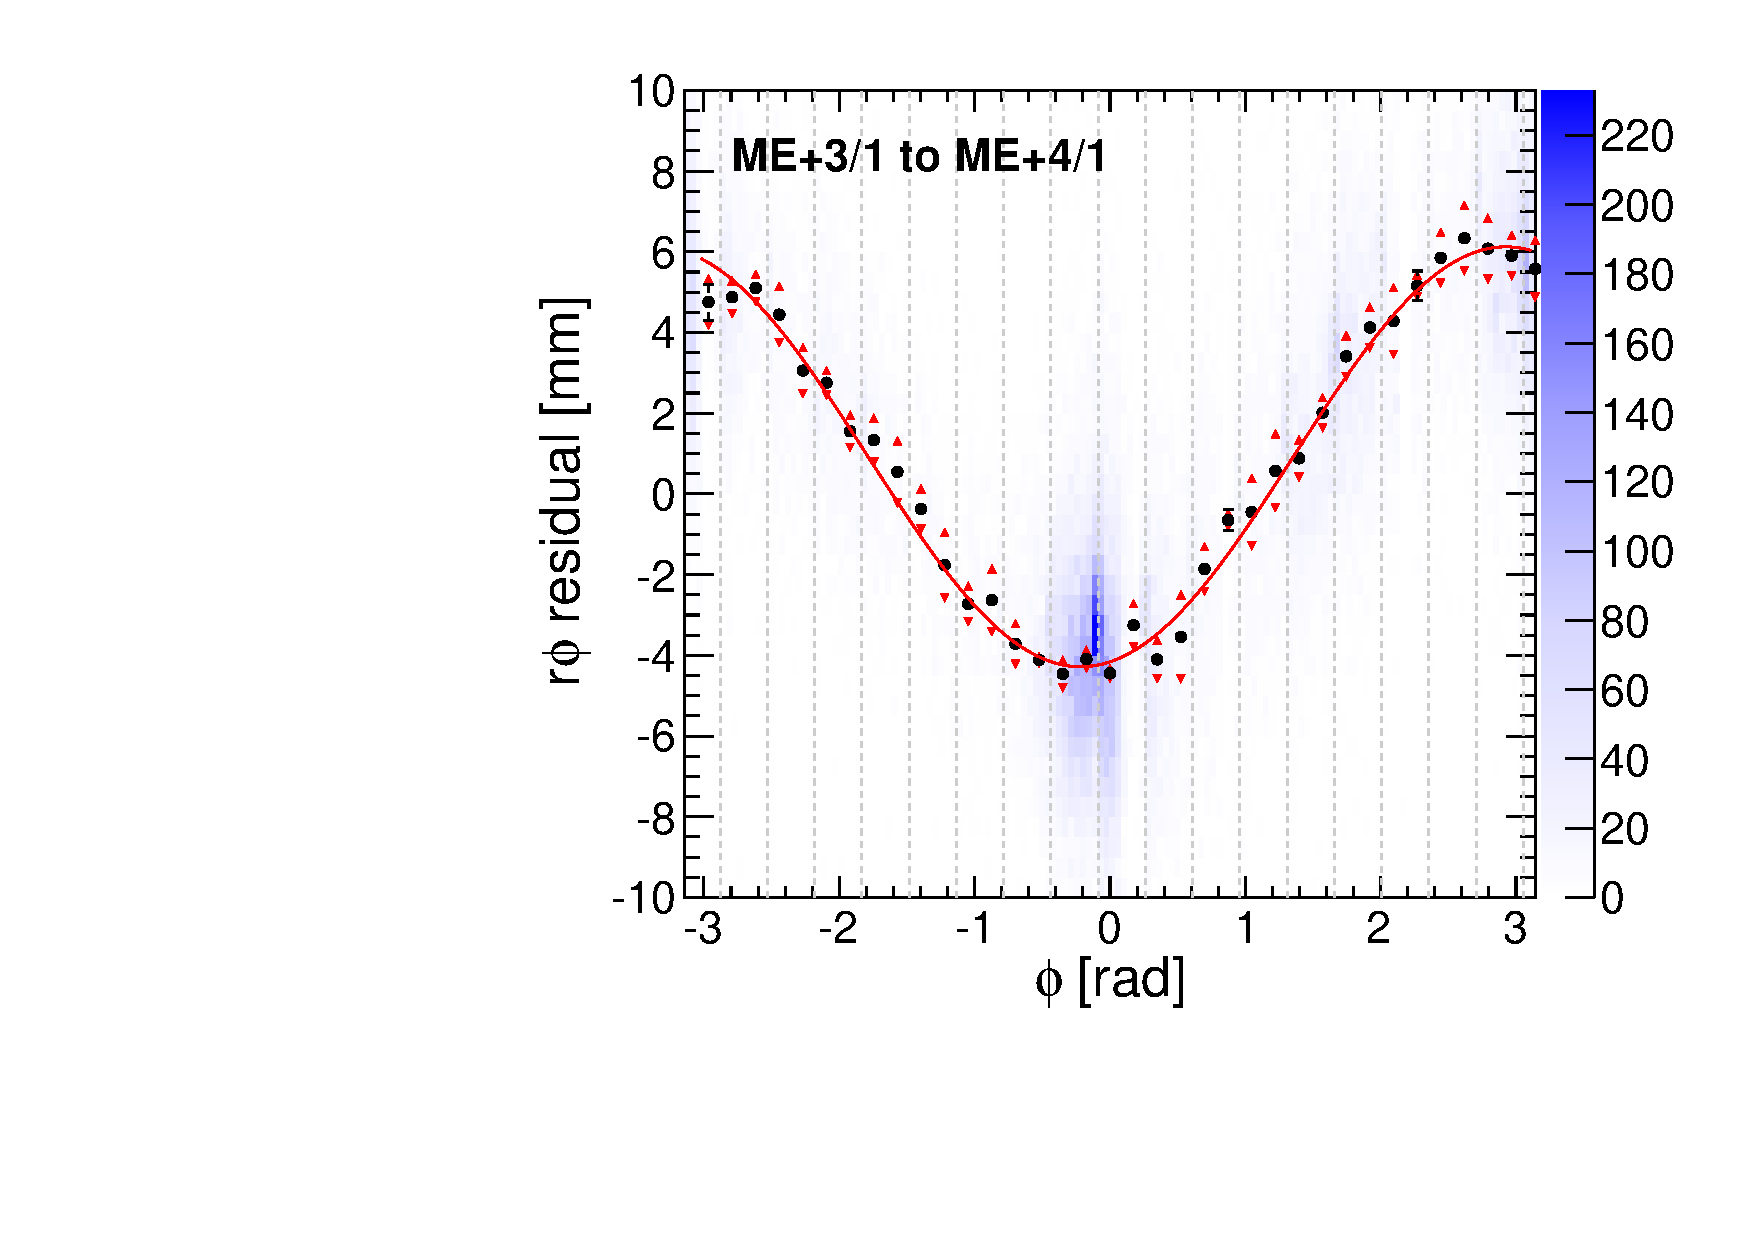
\includegraphics[width=0.4\linewidth]{BHCrossCheck_mep41_before.pdf}
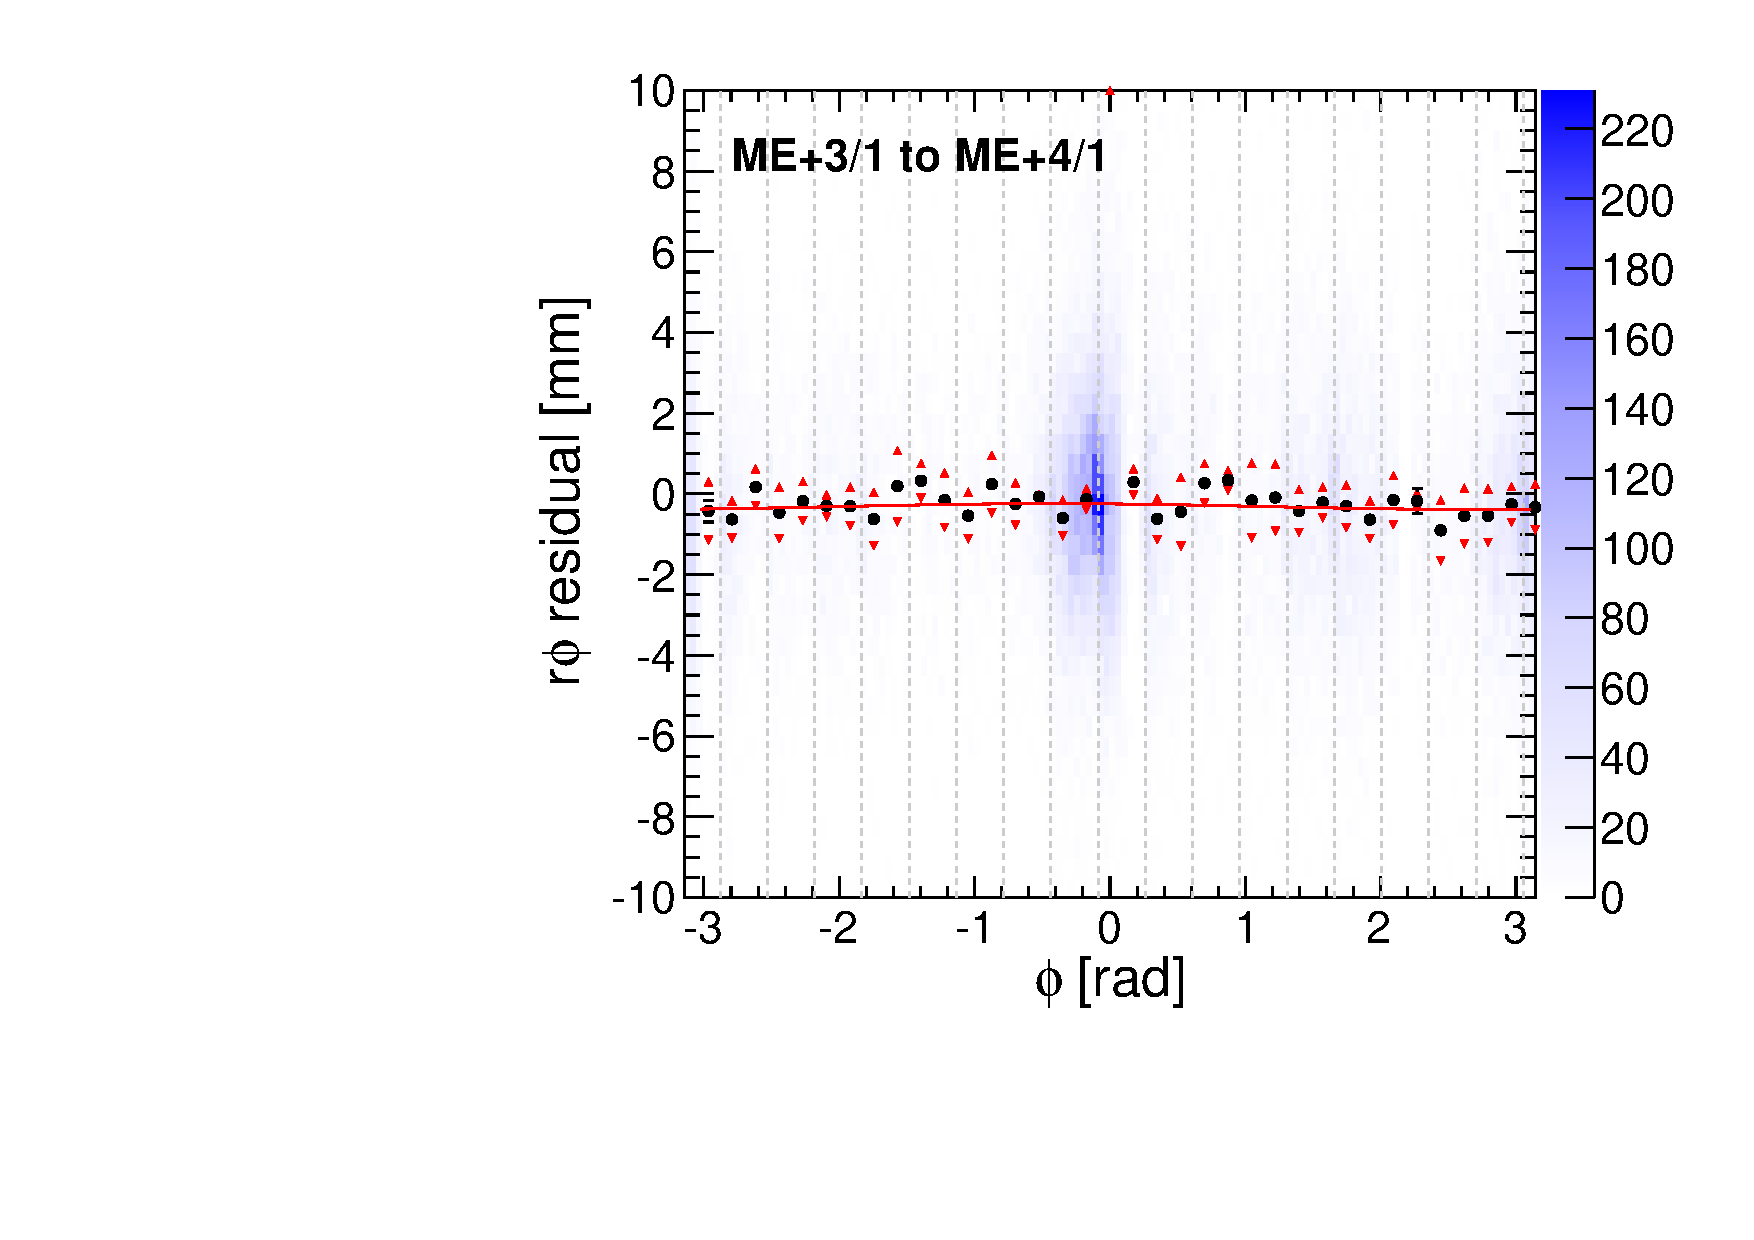
\includegraphics[width=0.4\linewidth]{BHCrossCheck_mep41_after.pdf}

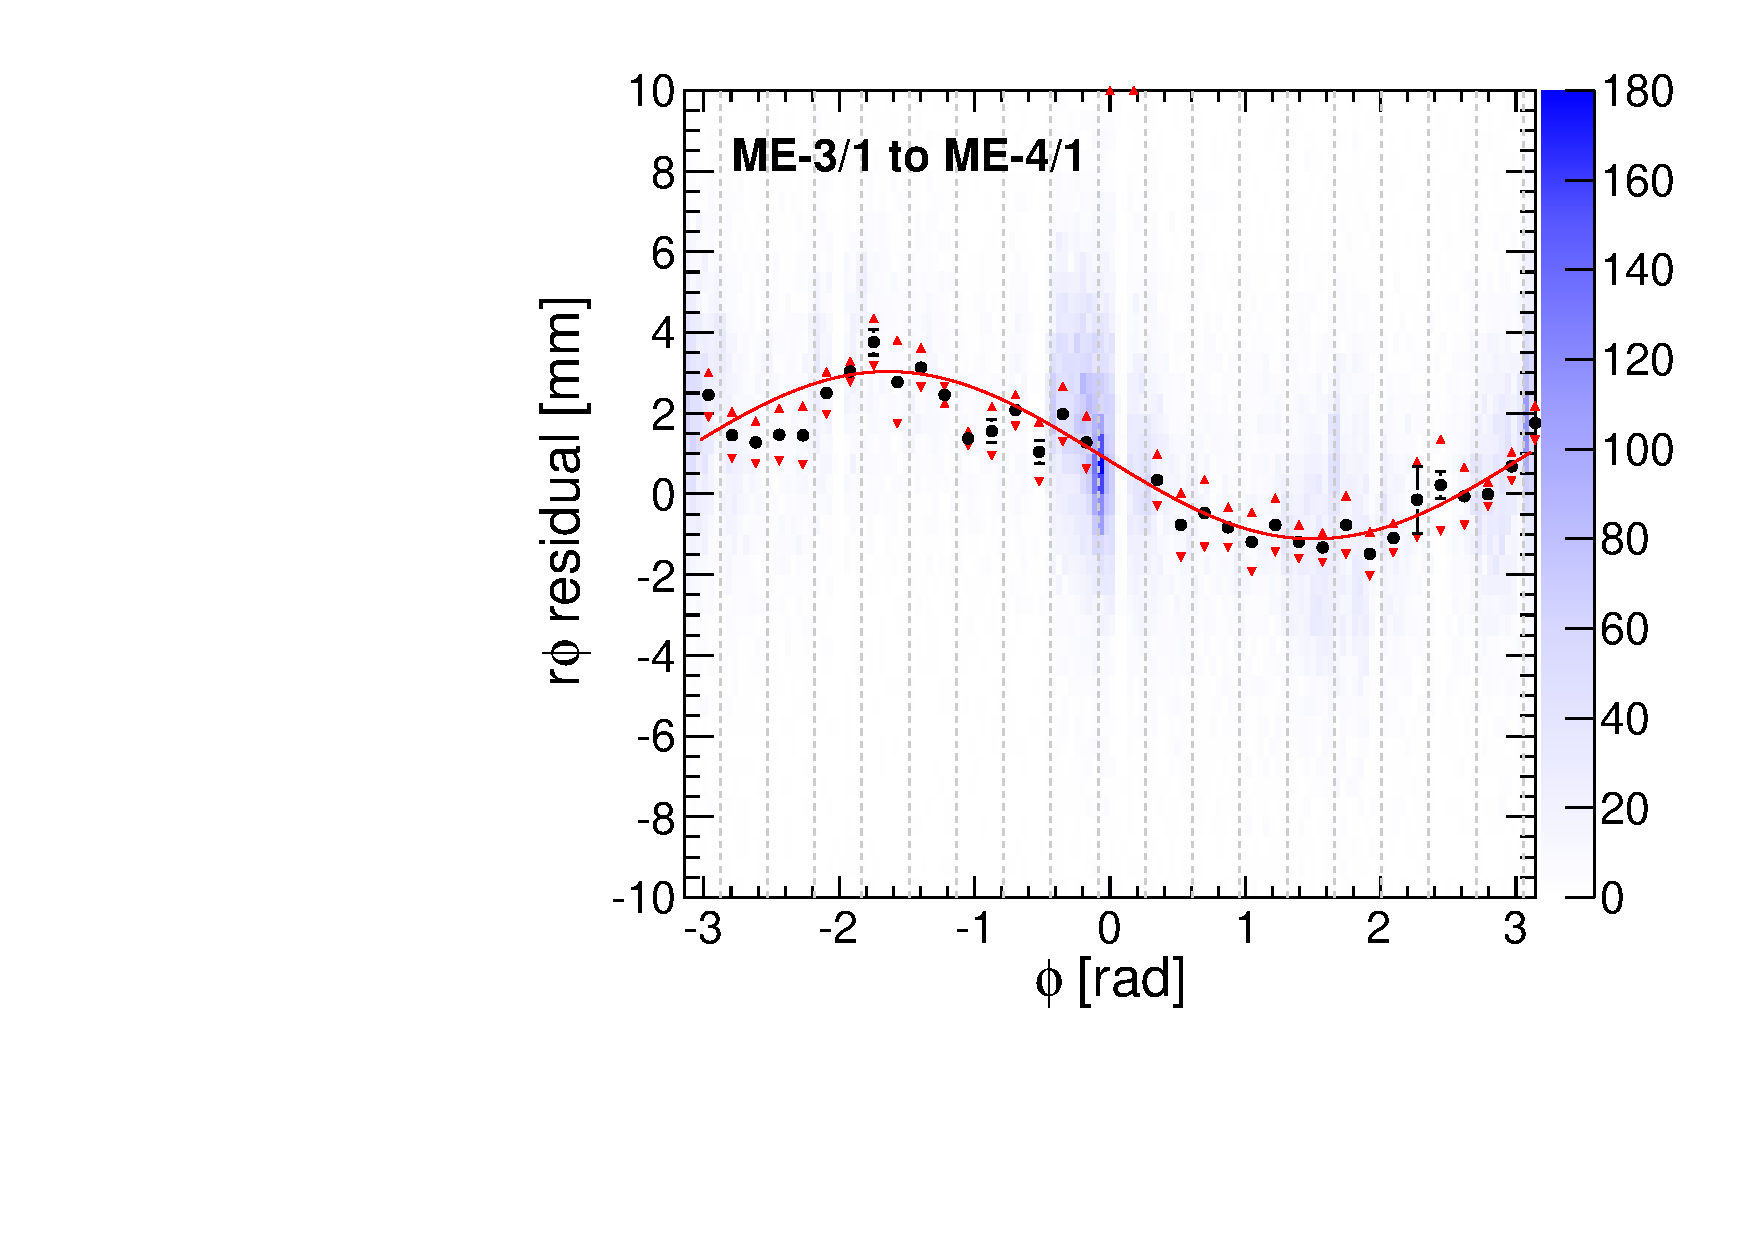
\includegraphics[width=0.4\linewidth]{BHCrossCheck_mem41_before.pdf}
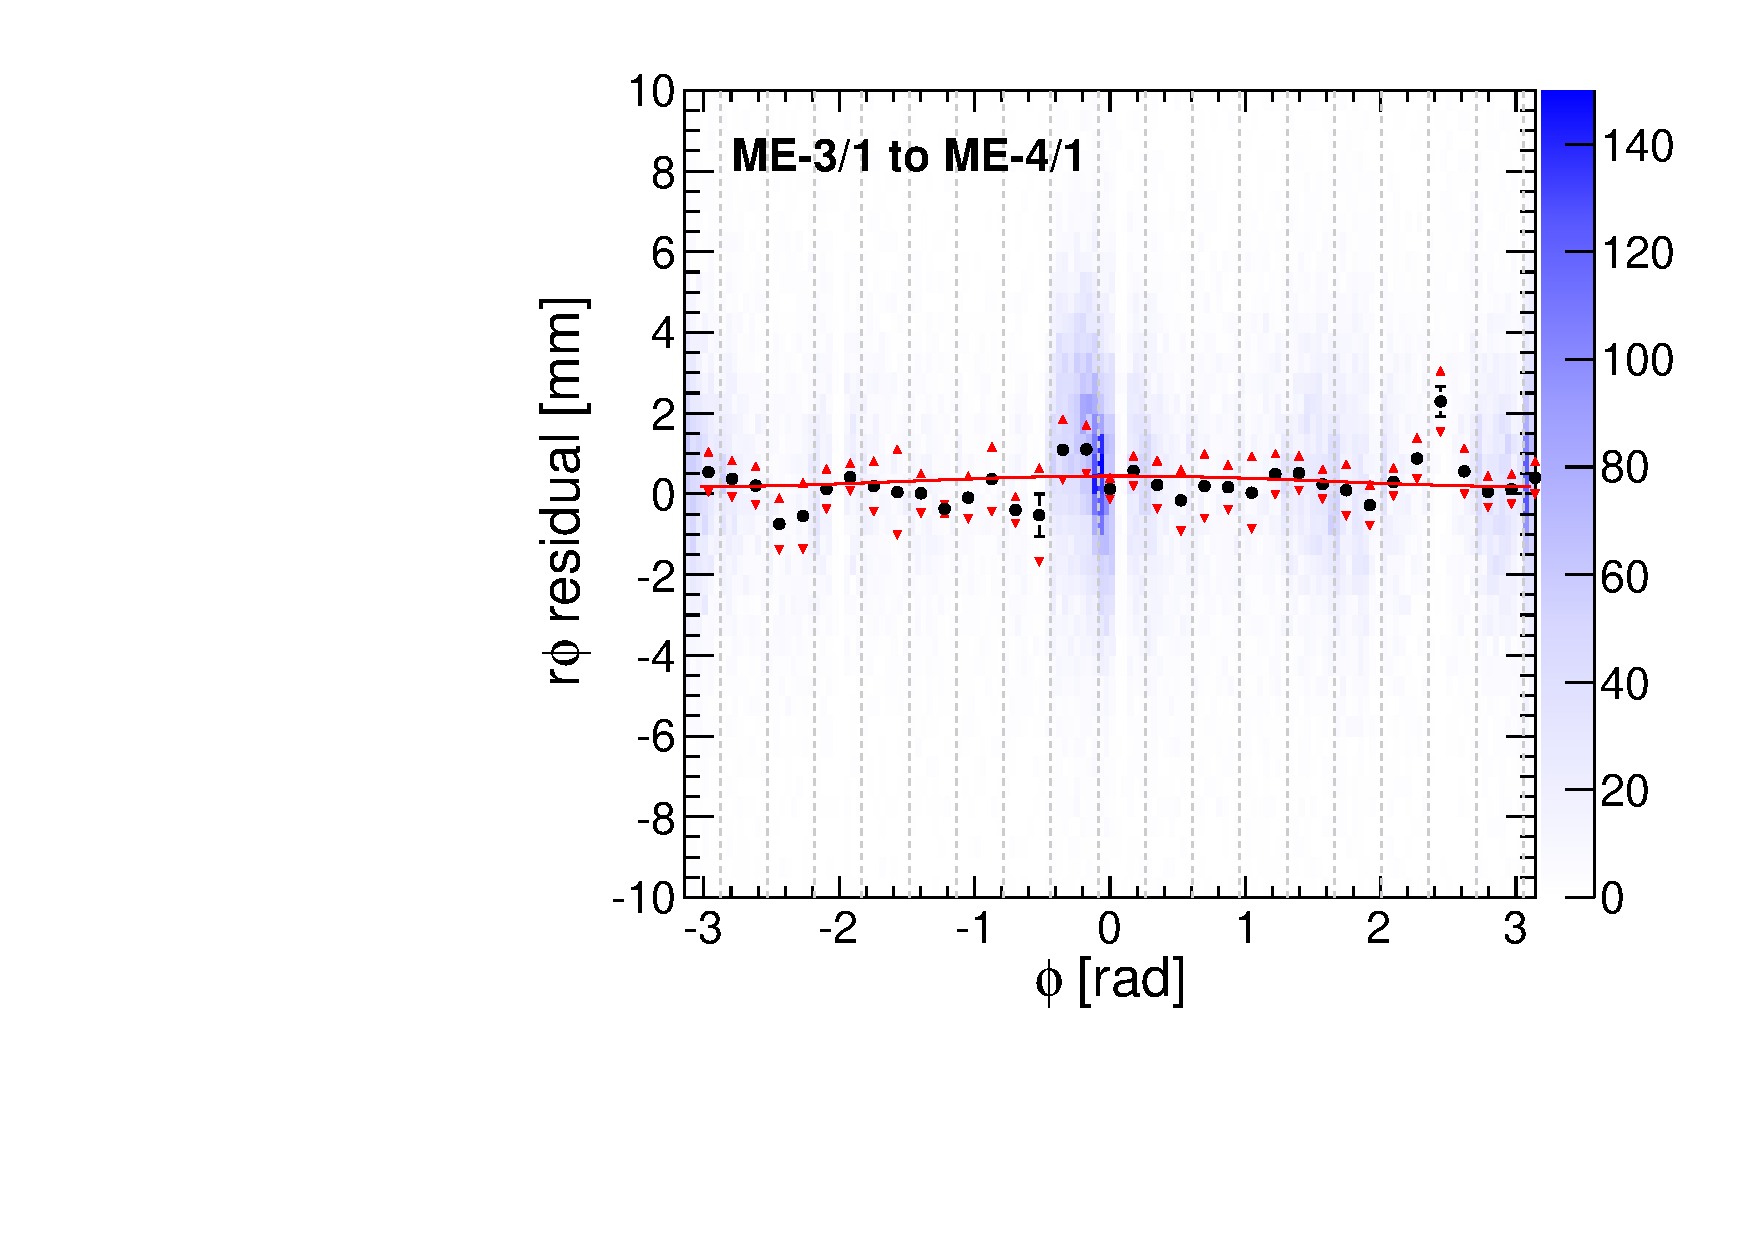
\includegraphics[width=0.4\linewidth]{BHCrossCheck_mem41_after.pdf}
\end{center}

\caption{Consistency of beam-halo segments linearly extrapolated from
  ME3/1 to ME4/1 with segments in ME4/1, before (left) and after
  (right) the independent tracker-to-muon ring alignment.  Red
  triangles are separate peak fits of positive $q\times p_z$ muons
  (upward-pointing triangles) and negative $q\times p_z$ muons
  (downward-pointing triangles), and black circles are the
  averages. \label{fig:BHCrossCheck_me41}}
\end{figure}

\begin{figure}
\begin{center}
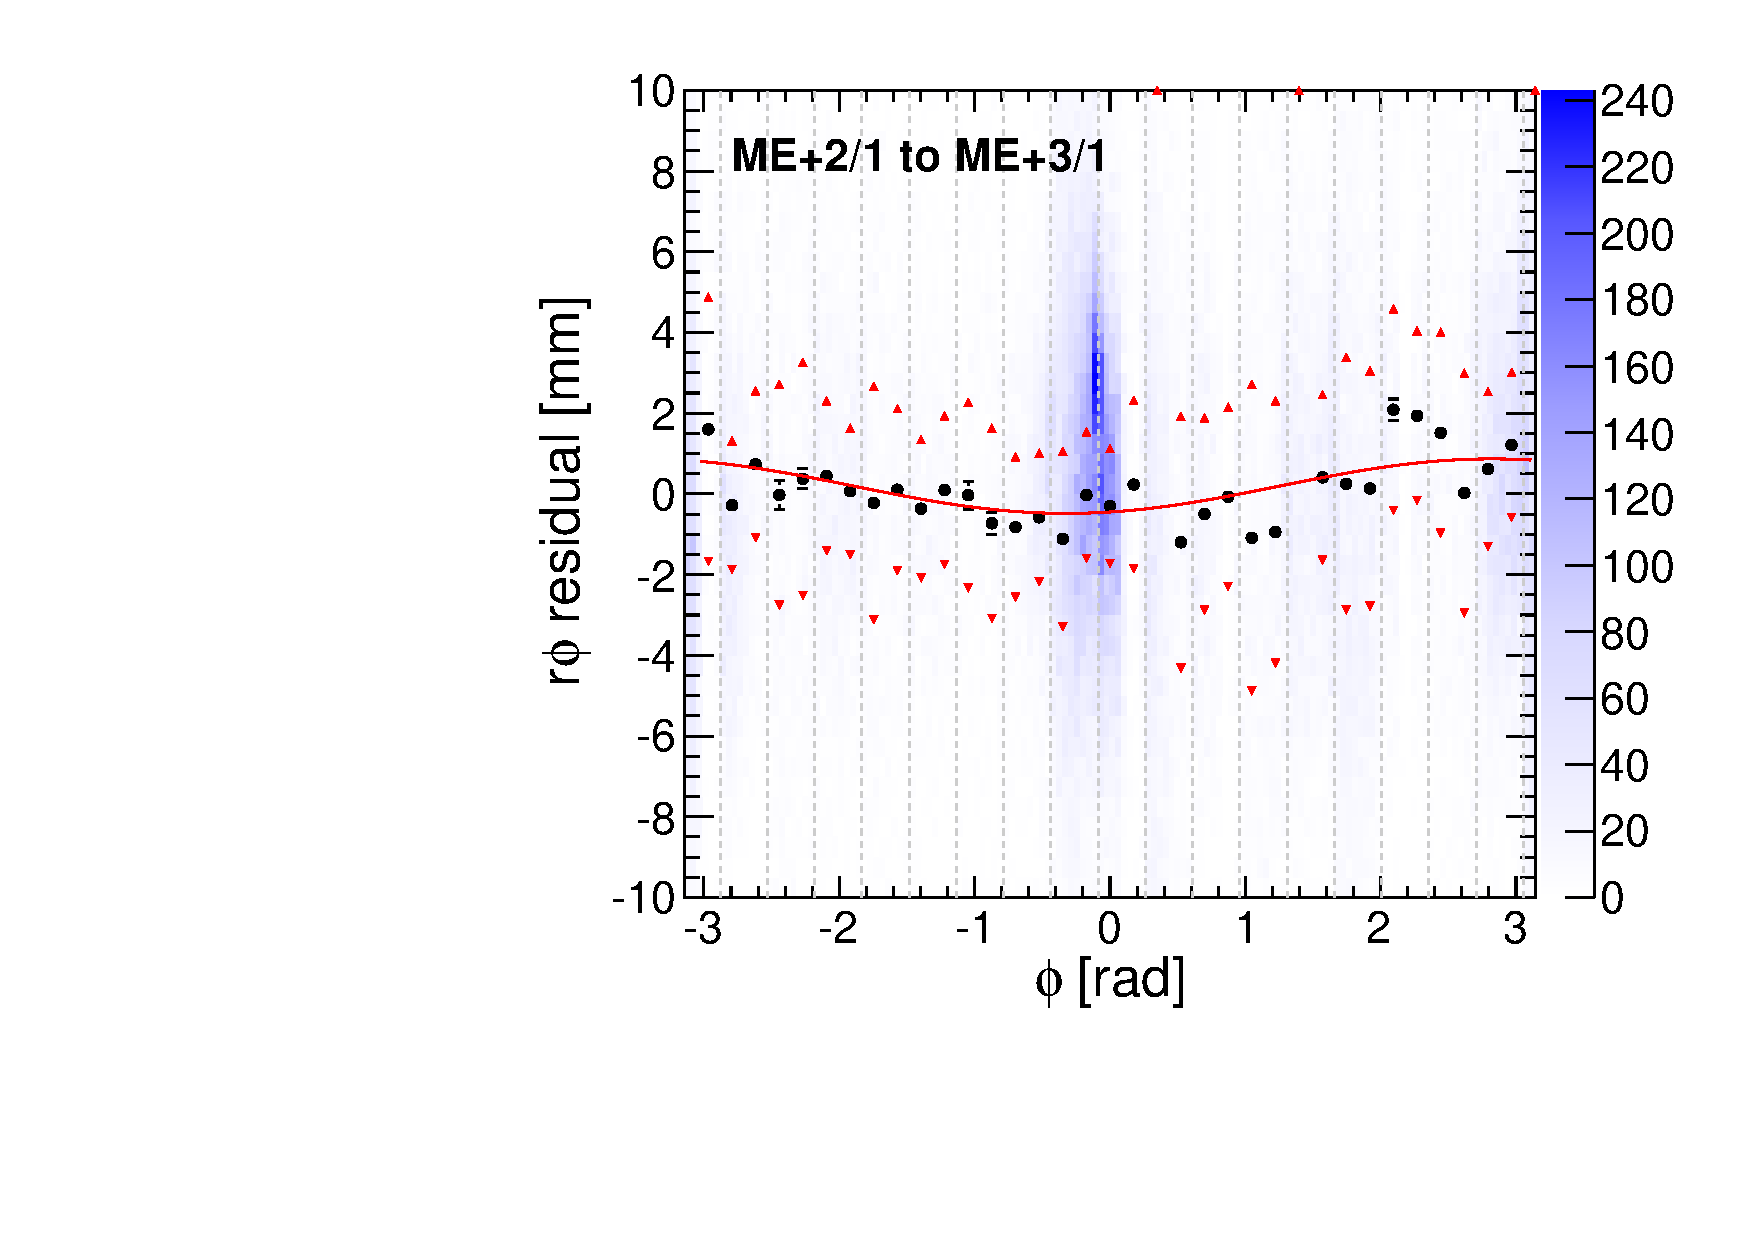
\includegraphics[width=0.4\linewidth]{BHCrossCheck_mep31_before.pdf}
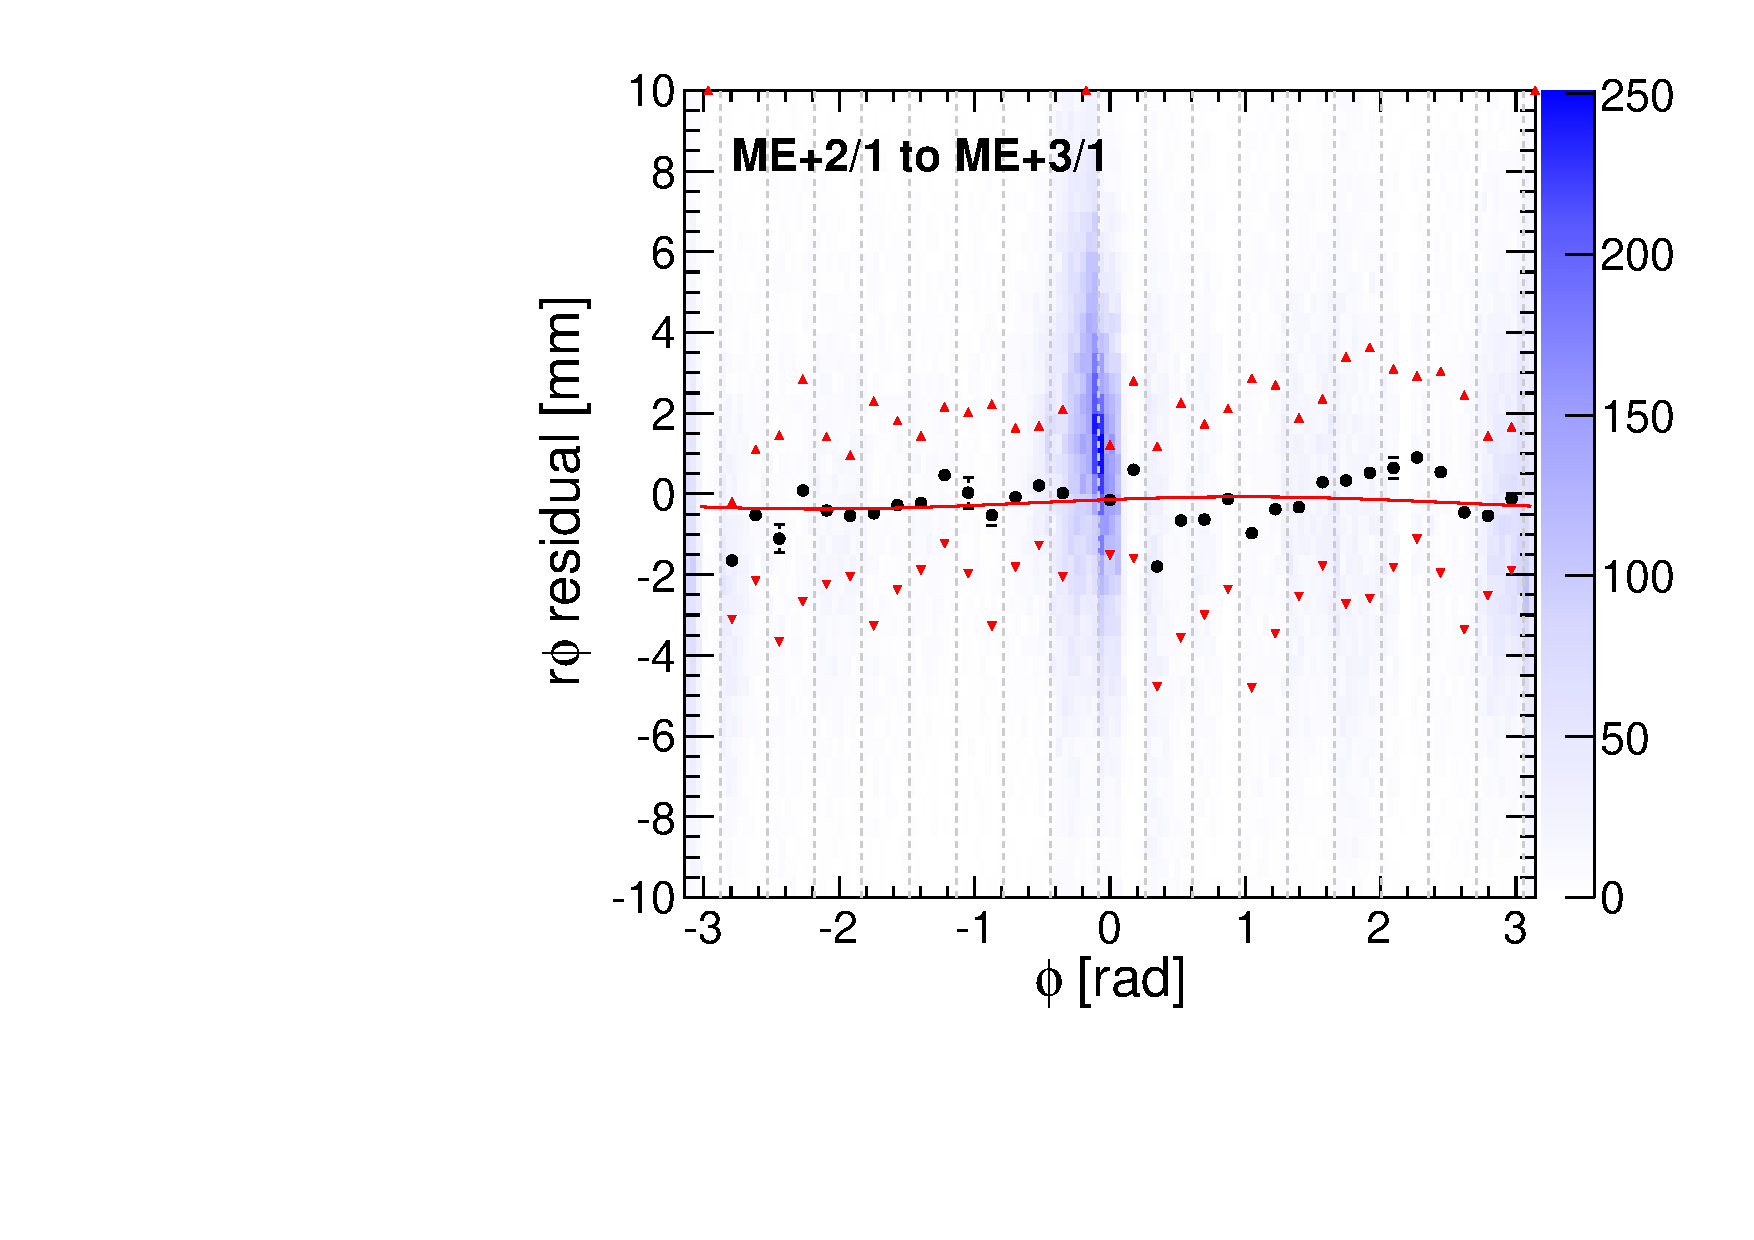
\includegraphics[width=0.4\linewidth]{BHCrossCheck_mep31_after.pdf}

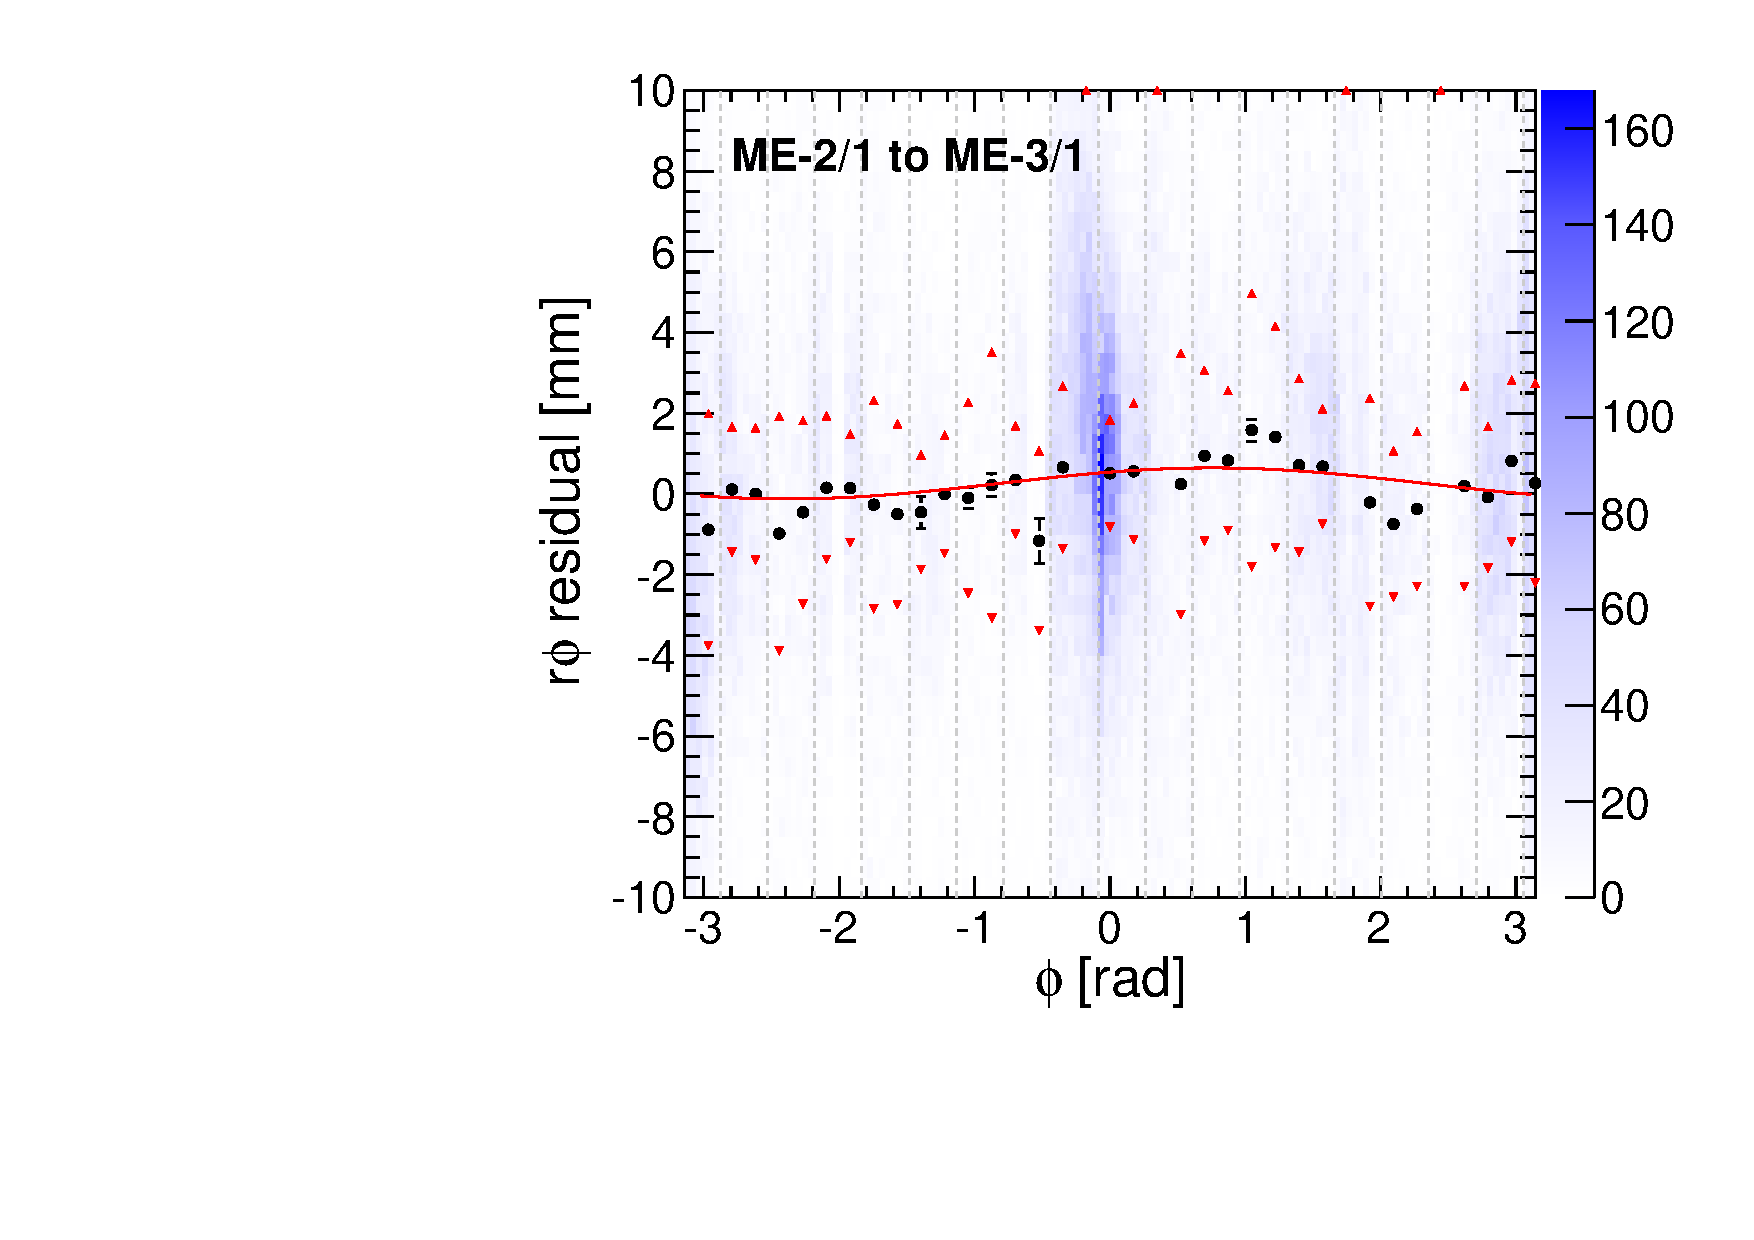
\includegraphics[width=0.4\linewidth]{BHCrossCheck_mem31_before.pdf}
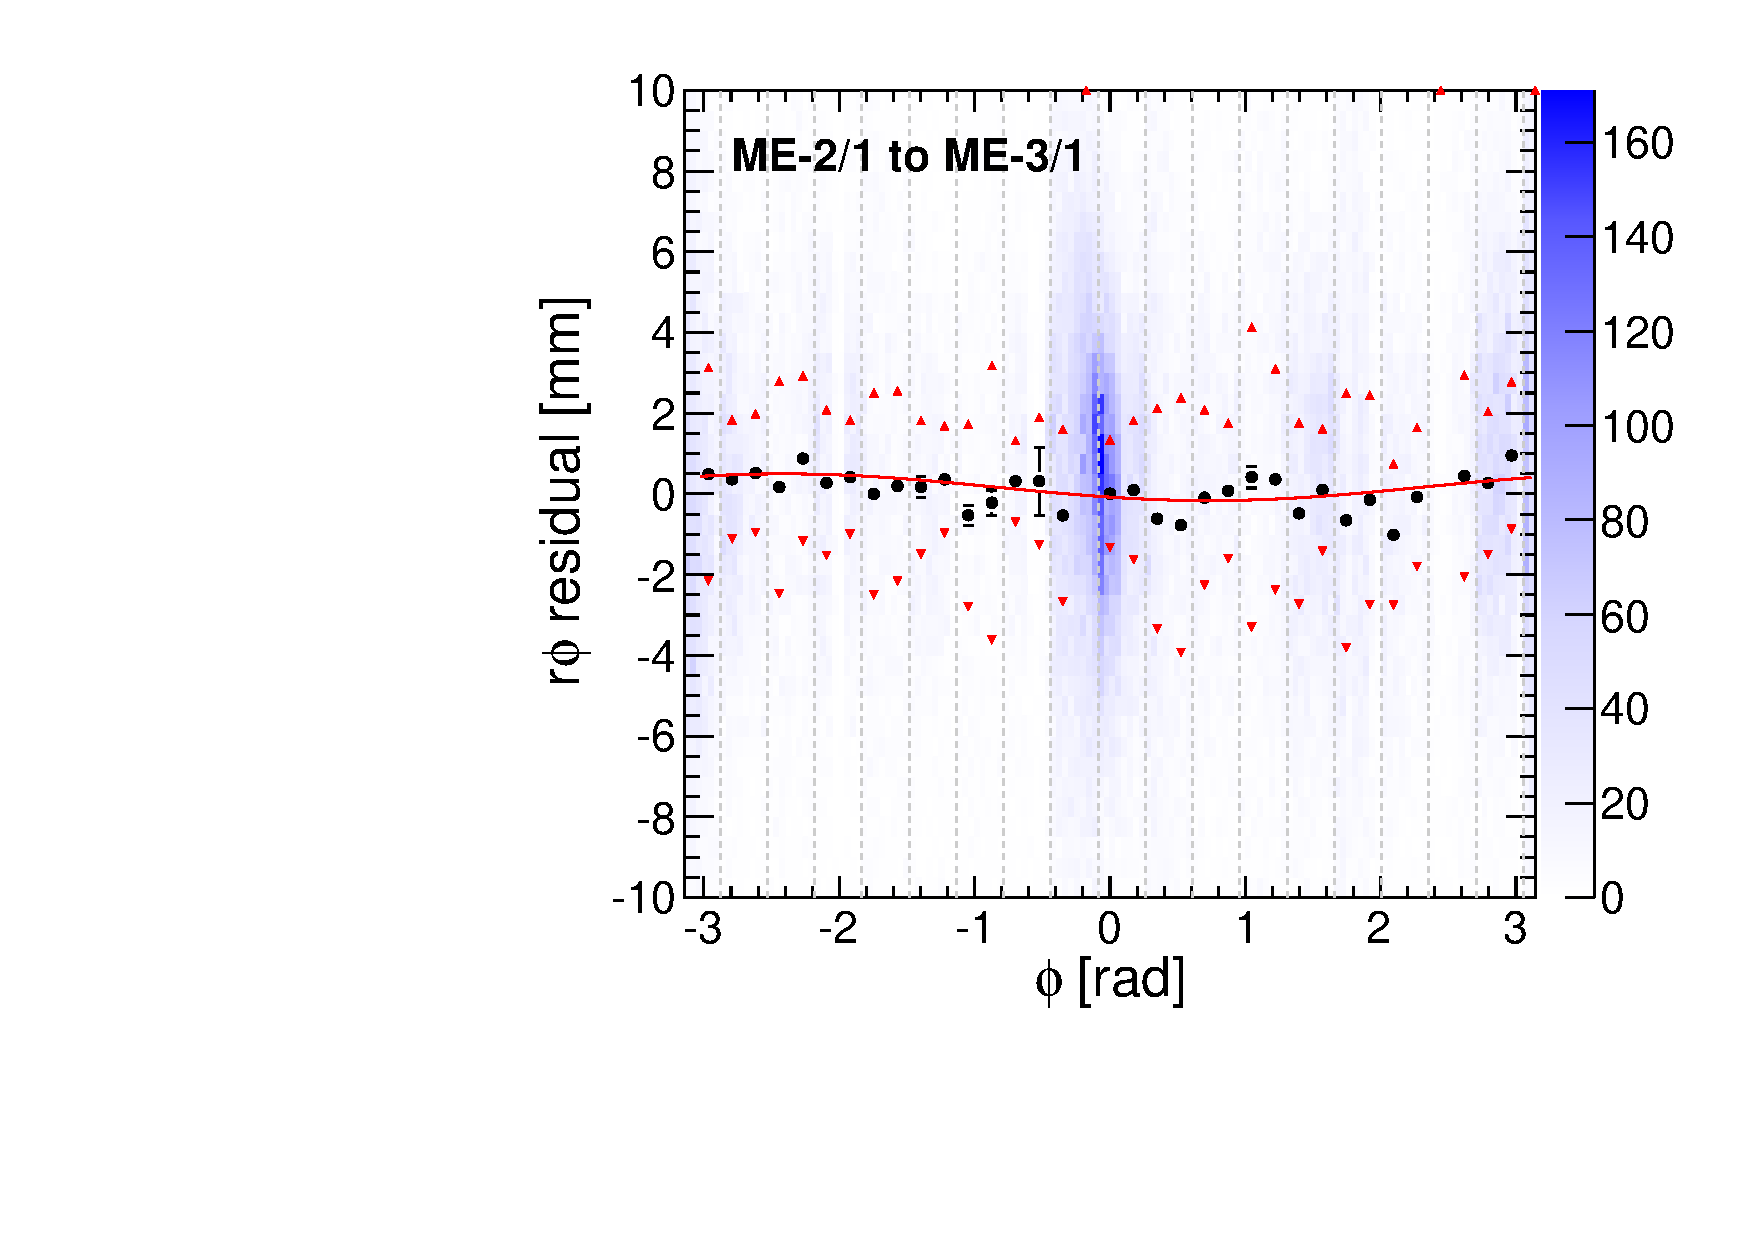
\includegraphics[width=0.4\linewidth]{BHCrossCheck_mem31_after.pdf}
\end{center}

\caption{Consistency of beam-halo segments linearly extrapolated from
  ME2/1 to ME3/1 with segments in ME3/1, before (left) and after
  (right) the independent tracker-to-muon ring alignment.  (See
  Fig.~\ref{fig:BHCrossCheck_me41} for additional explanation.)  Large
  corrections were not expected (or observed) before alignment, as the
  ME2 and ME3 stations are connected to the same physical
  disk. \label{fig:BHCrossCheck_me31}}
\end{figure}

\begin{figure}
\begin{center}
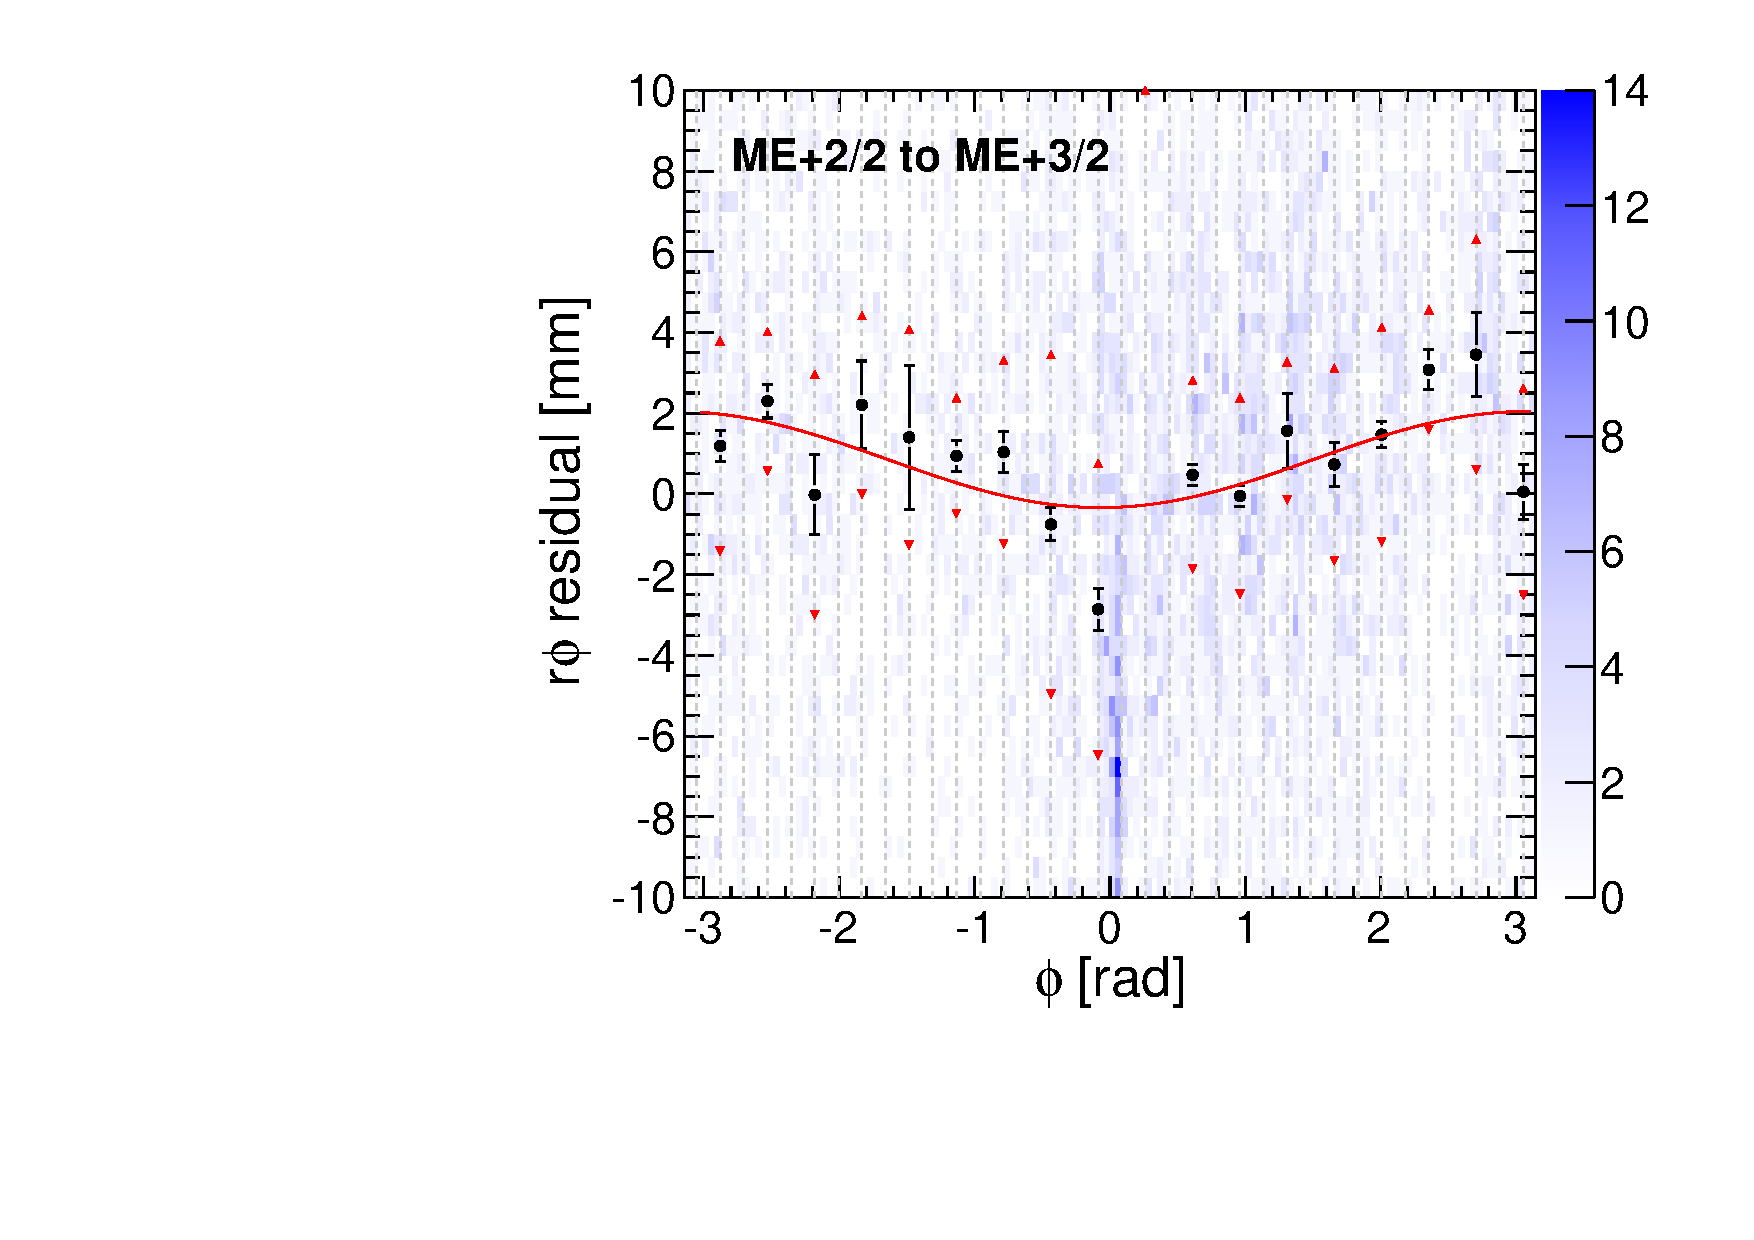
\includegraphics[width=0.4\linewidth]{BHCrossCheck_mep32_before.pdf}
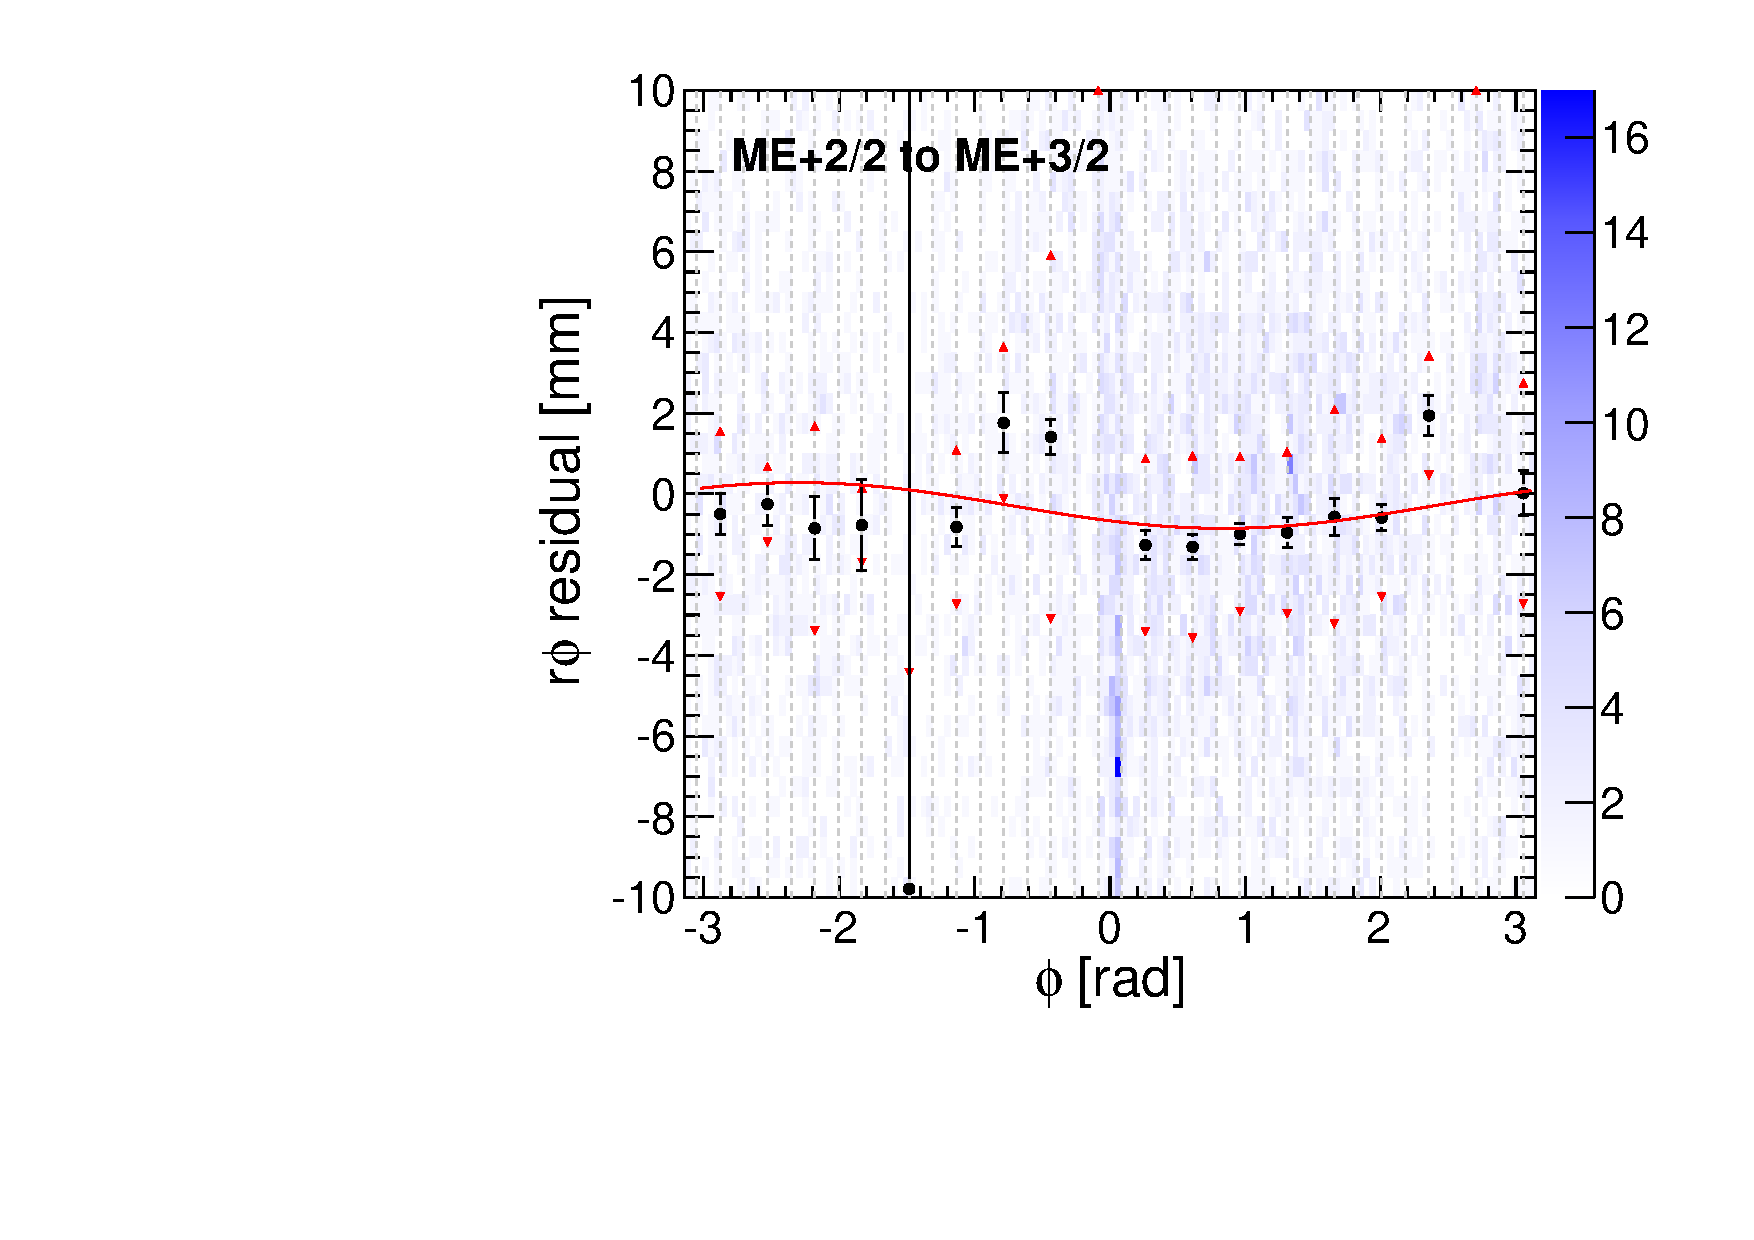
\includegraphics[width=0.4\linewidth]{BHCrossCheck_mep32_after.pdf}

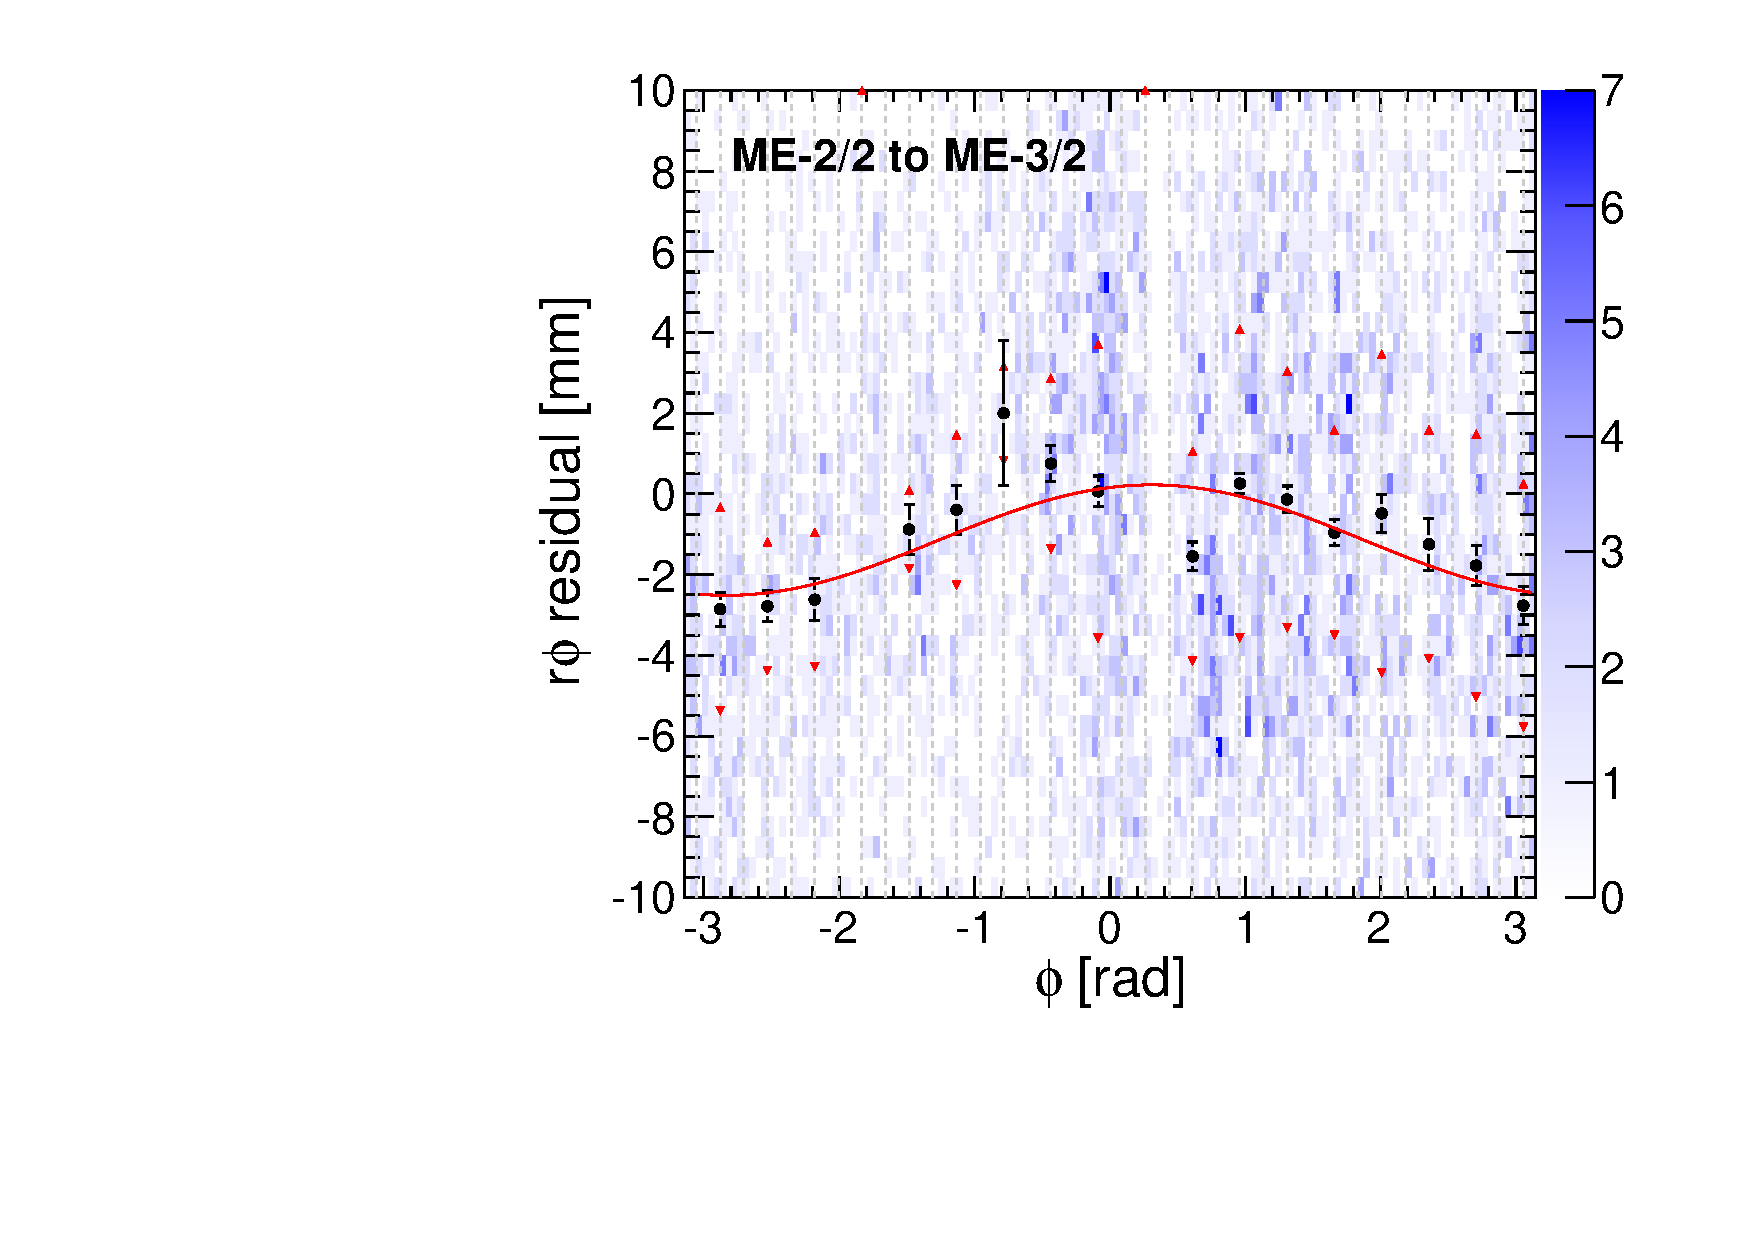
\includegraphics[width=0.4\linewidth]{BHCrossCheck_mem32_before.pdf}
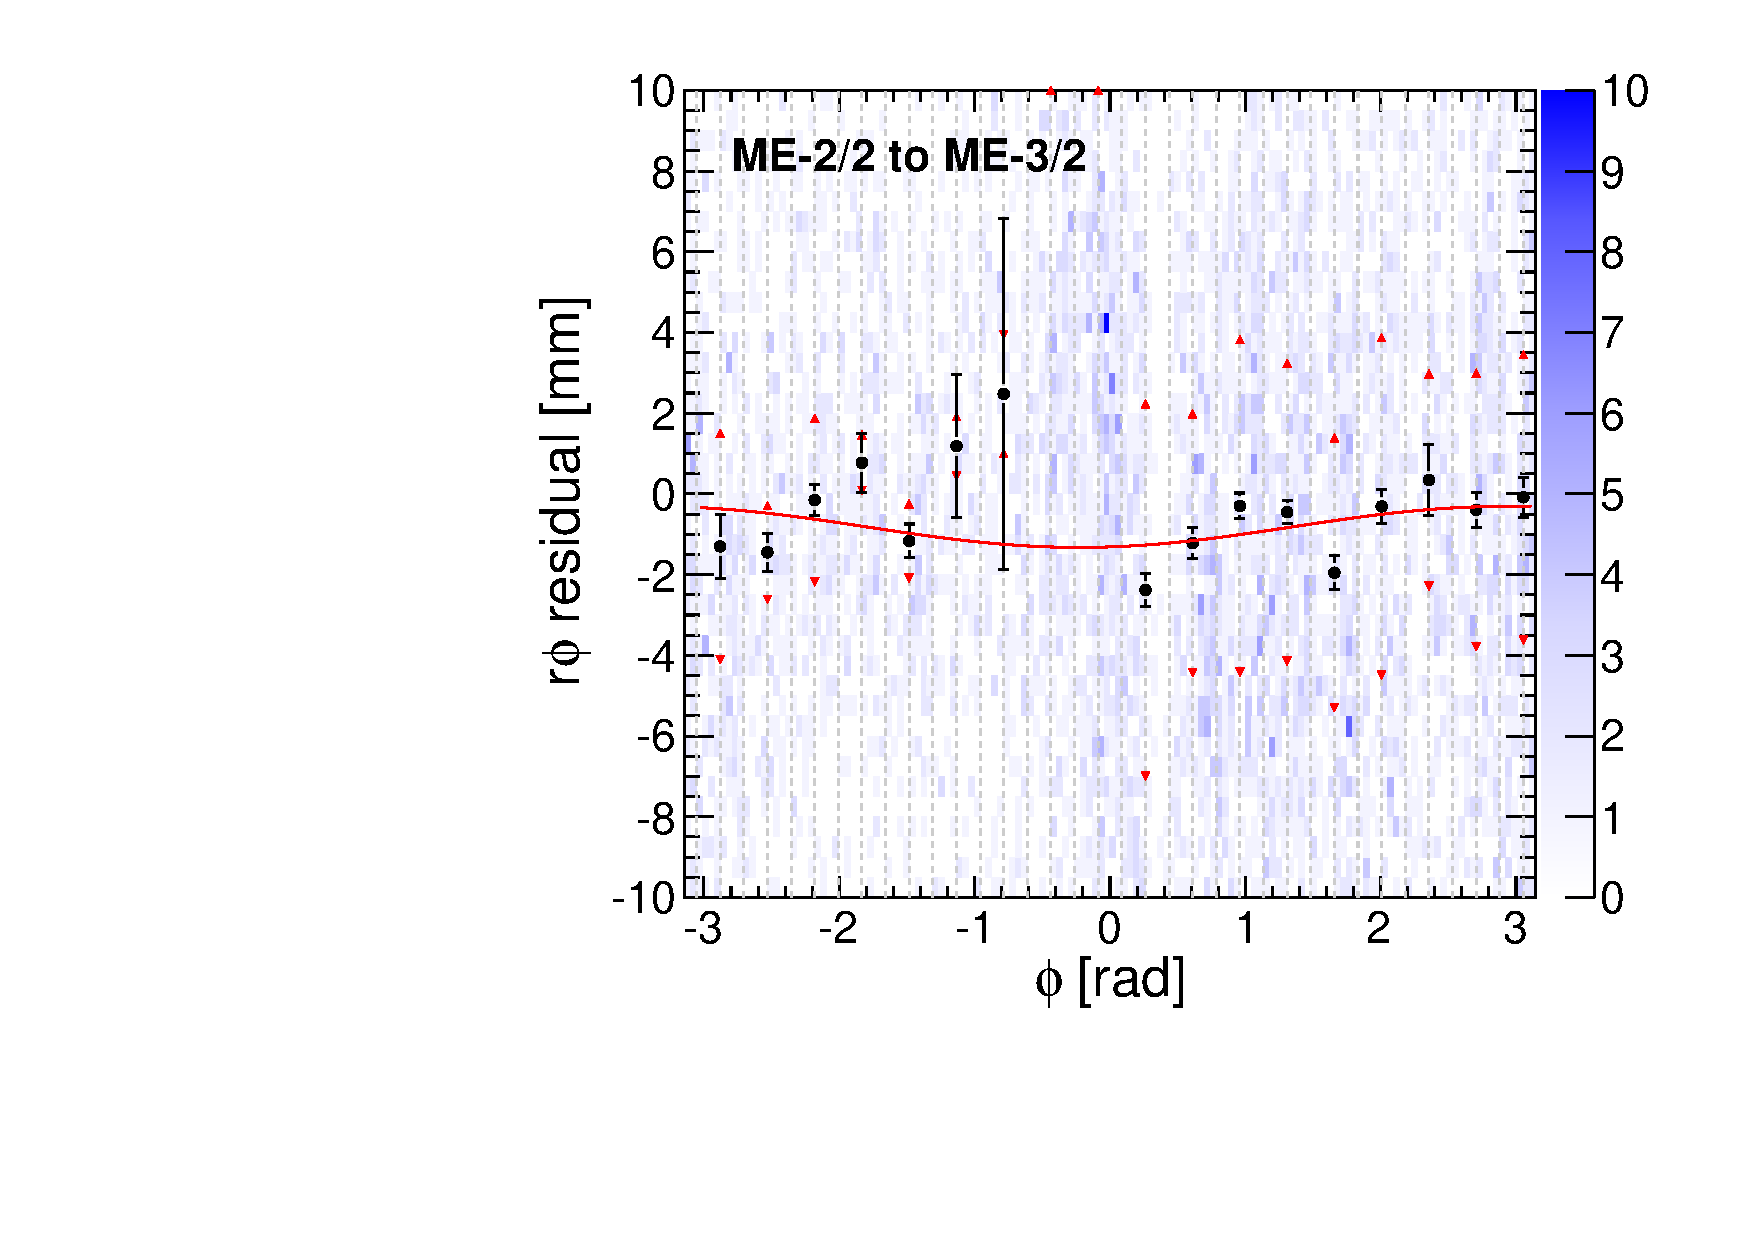
\includegraphics[width=0.4\linewidth]{BHCrossCheck_mem32_after.pdf}
\end{center}

\caption{Consistency of beam-halo segments linearly extrapolated from
  ME2/2 to ME3/2 with segments in ME3/2, before (left) and after
  (right) the independent tracker-to-muon ring alignment.  (See
  Fig.~\ref{fig:BHCrossCheck_me41} for additional explanation.)  Large
  corrections were not expected (or observed) before alignment, as the
  ME2 and ME3 stations are connected to the same physical disk.
  (Outer rings like ME2/2 and ME3/3 have poor beam-halo
  statistics.) \label{fig:BHCrossCheck_me32}}
\end{figure}

\begin{figure}
\begin{center}
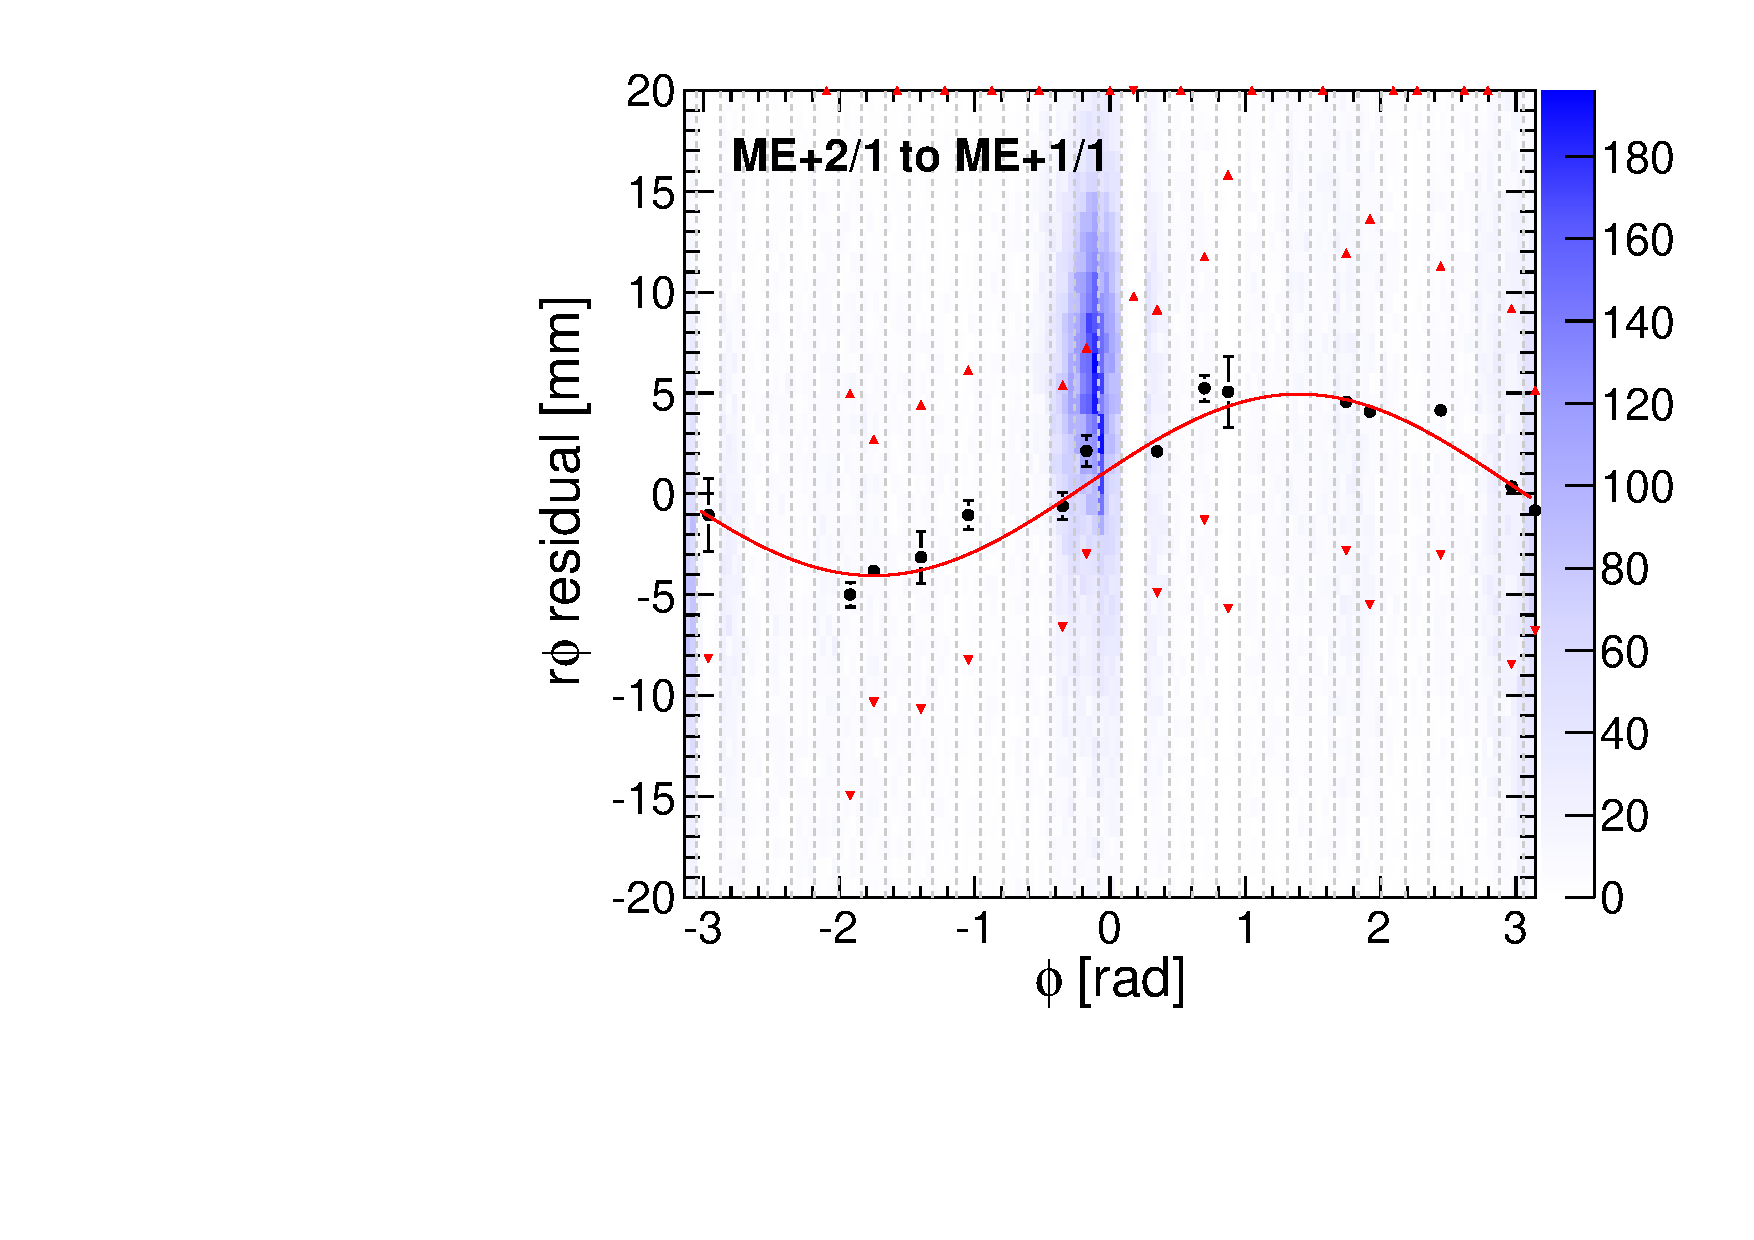
\includegraphics[width=0.4\linewidth]{BHCrossCheck_mep11_before.pdf}
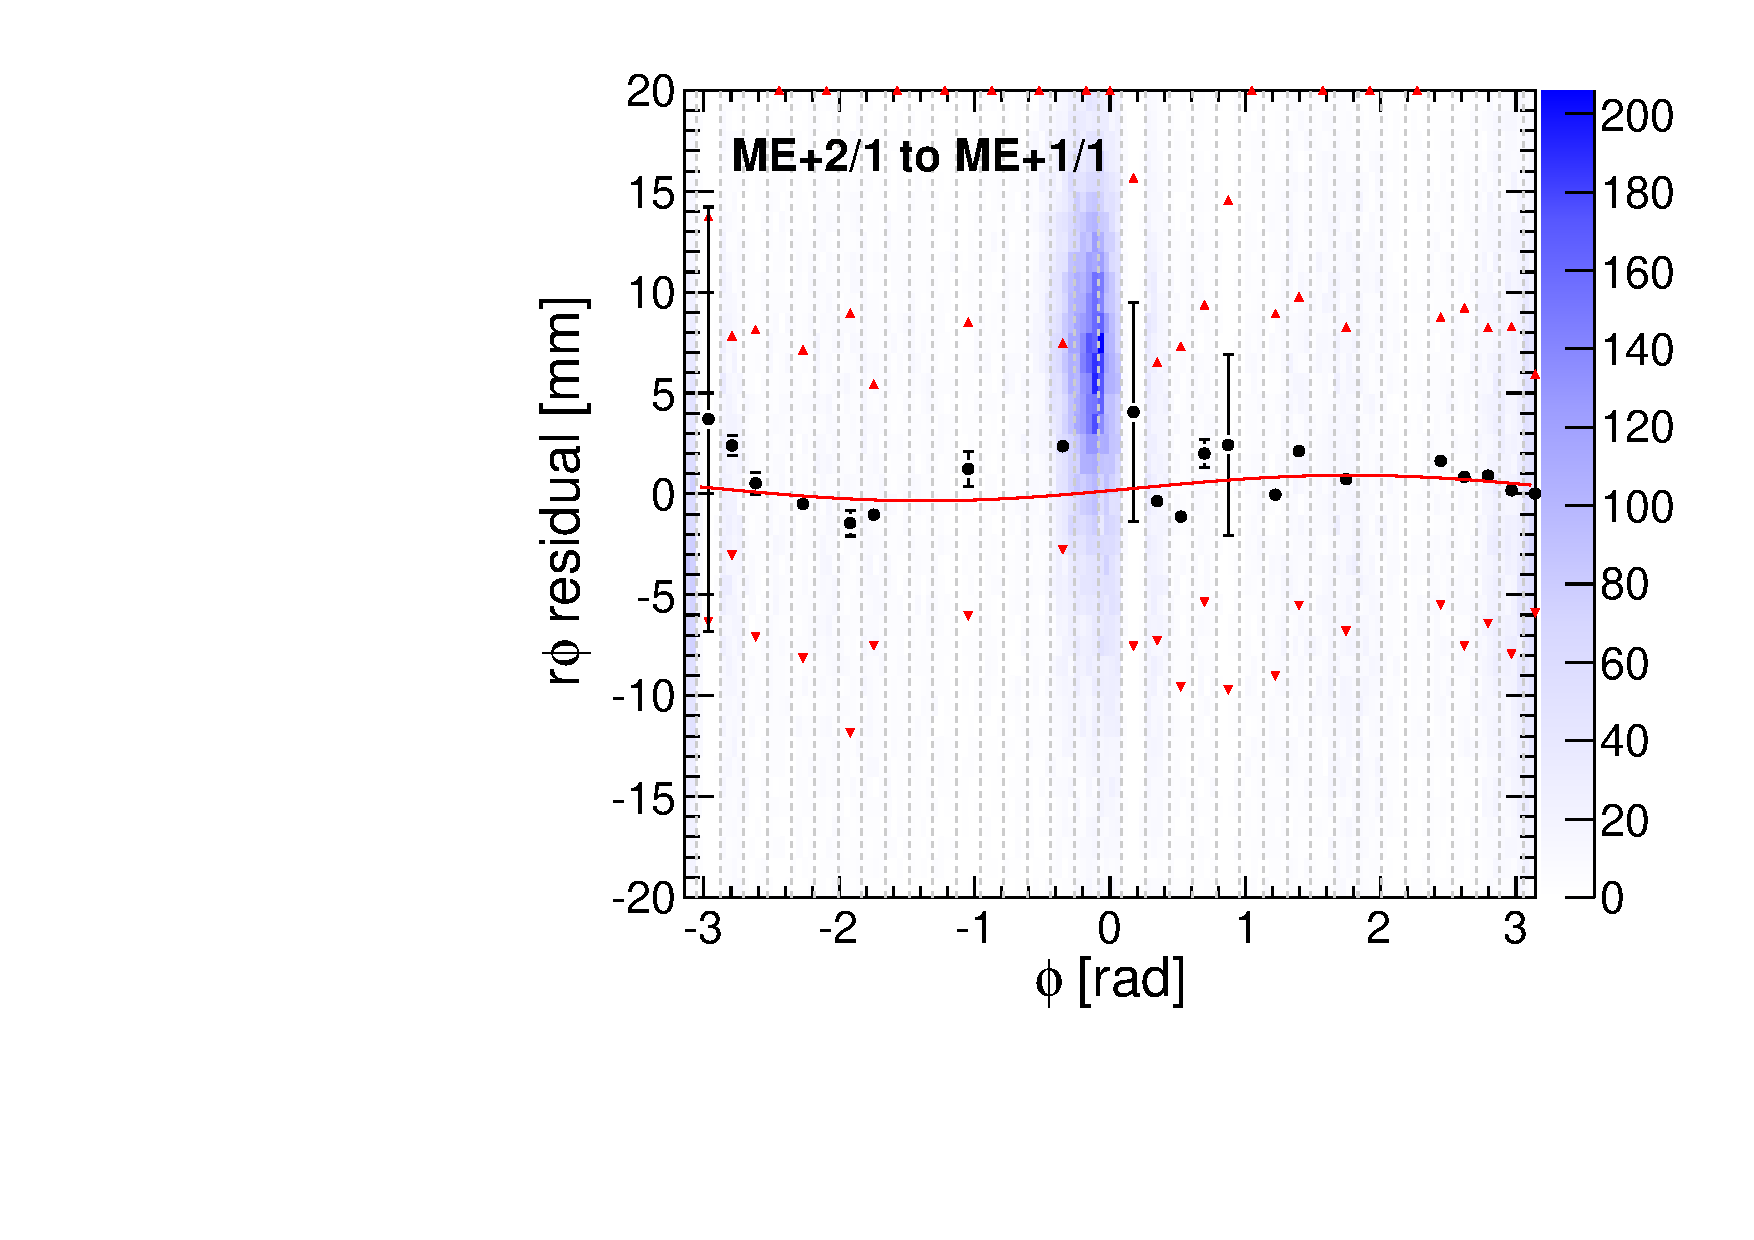
\includegraphics[width=0.4\linewidth]{BHCrossCheck_mep11_after.pdf}

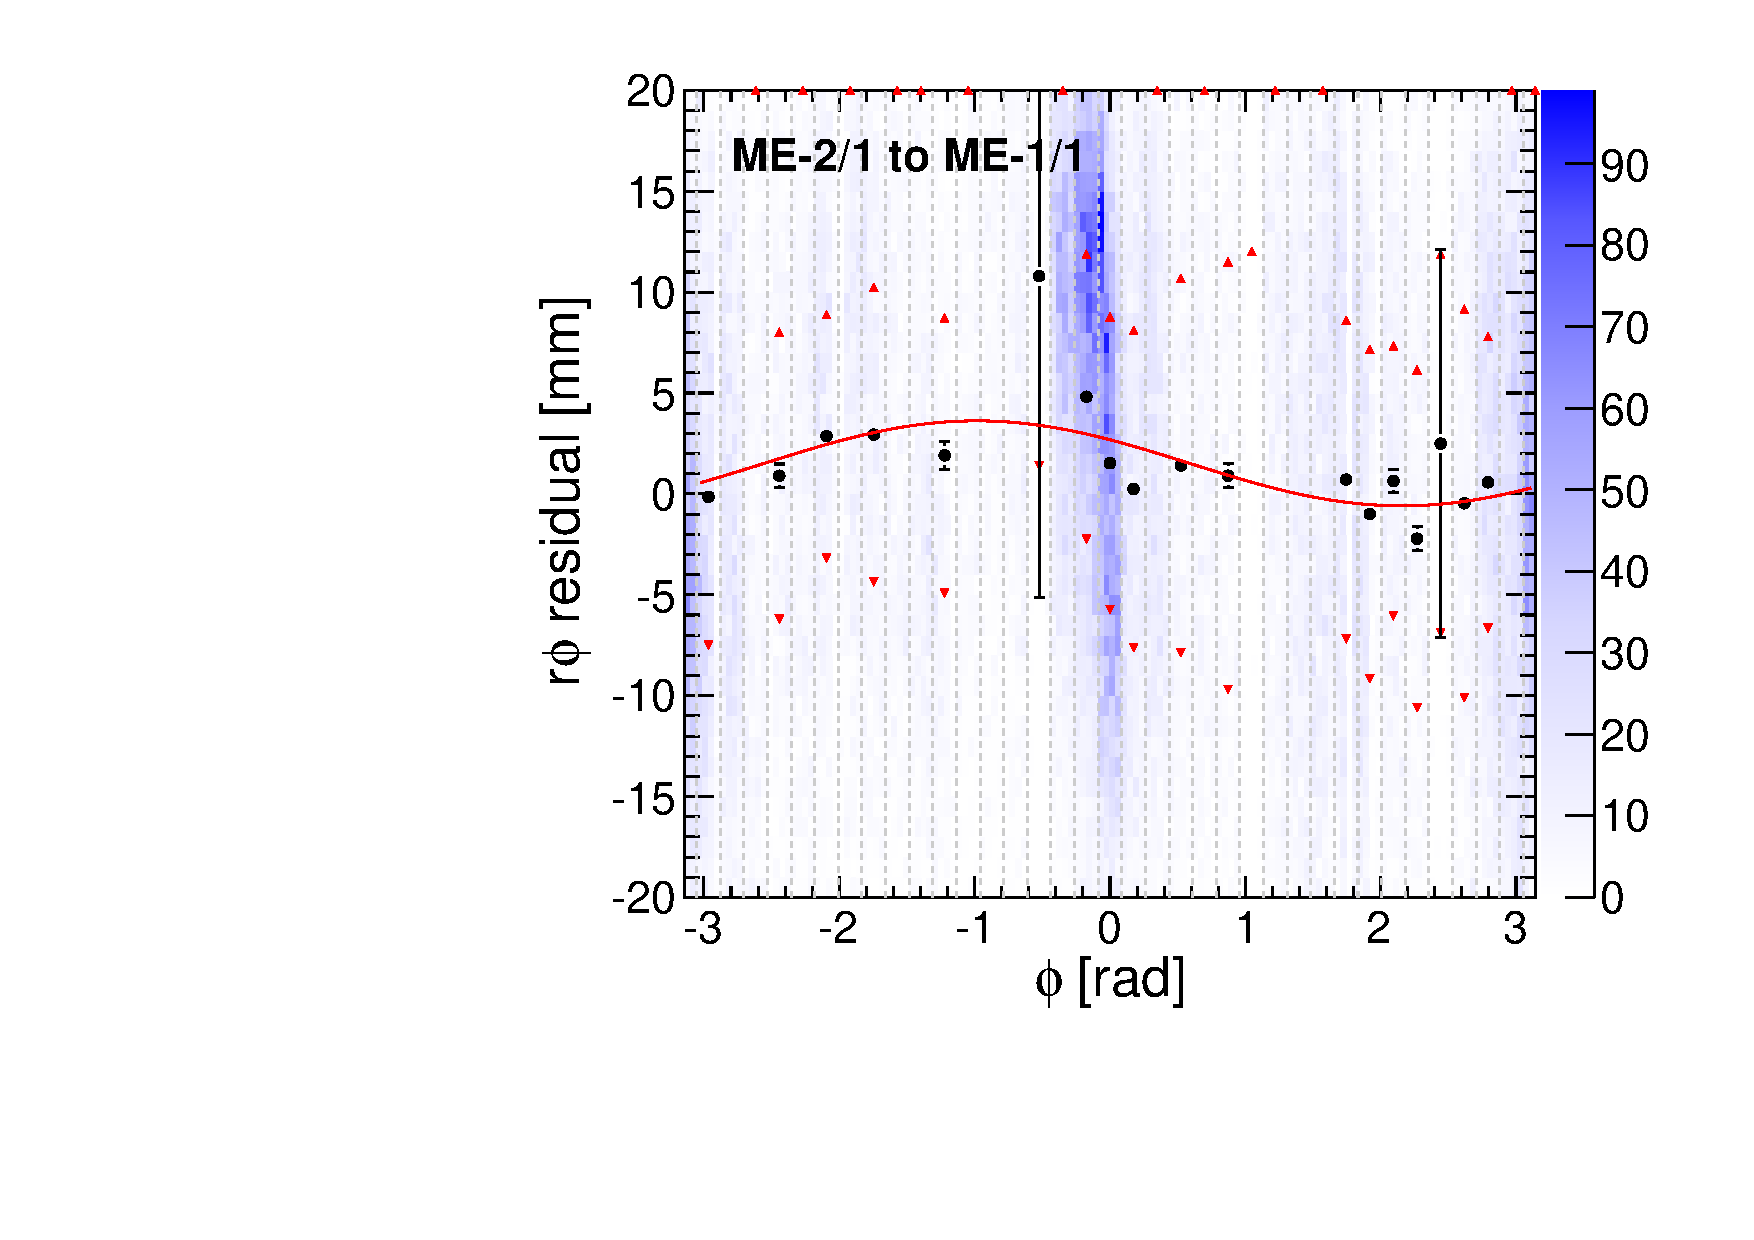
\includegraphics[width=0.4\linewidth]{BHCrossCheck_mem11_before.pdf}
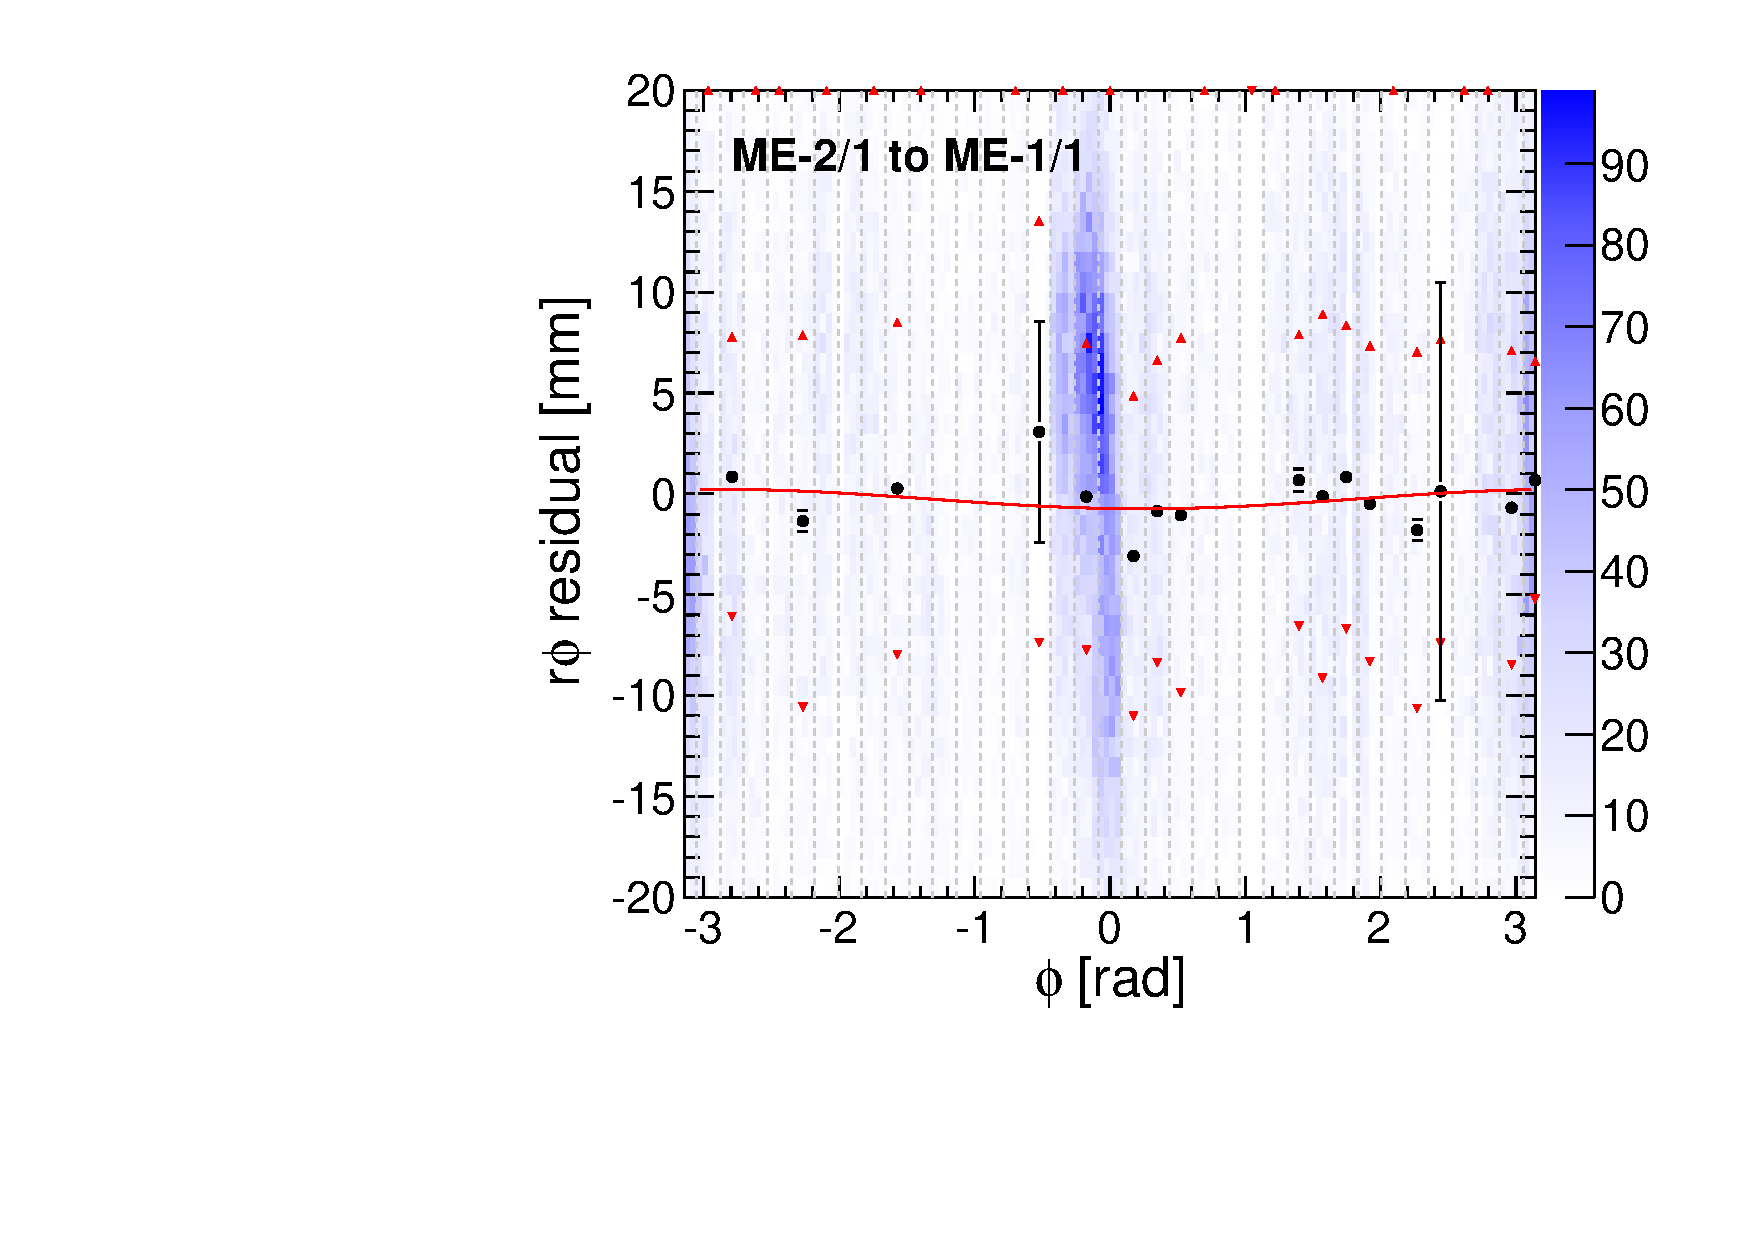
\includegraphics[width=0.4\linewidth]{BHCrossCheck_mem11_after.pdf}
\end{center}

\caption{Consistency of beam-halo segments linearly extrapolated from
  ME2/1 to ME1/1 with segments in ME1/1, before (left) and after
  (right) the independent tracker-to-muon ring alignment.  (See
  Fig.~\ref{fig:BHCrossCheck_me41} for additional explanation.)
  Differences between muons and antimuons (red triangles) are large
  because the radial magnetic field was not taken into account when
  propagating segments between stations. \label{fig:BHCrossCheck_me11}}
\end{figure}

\begin{figure}
\begin{center}
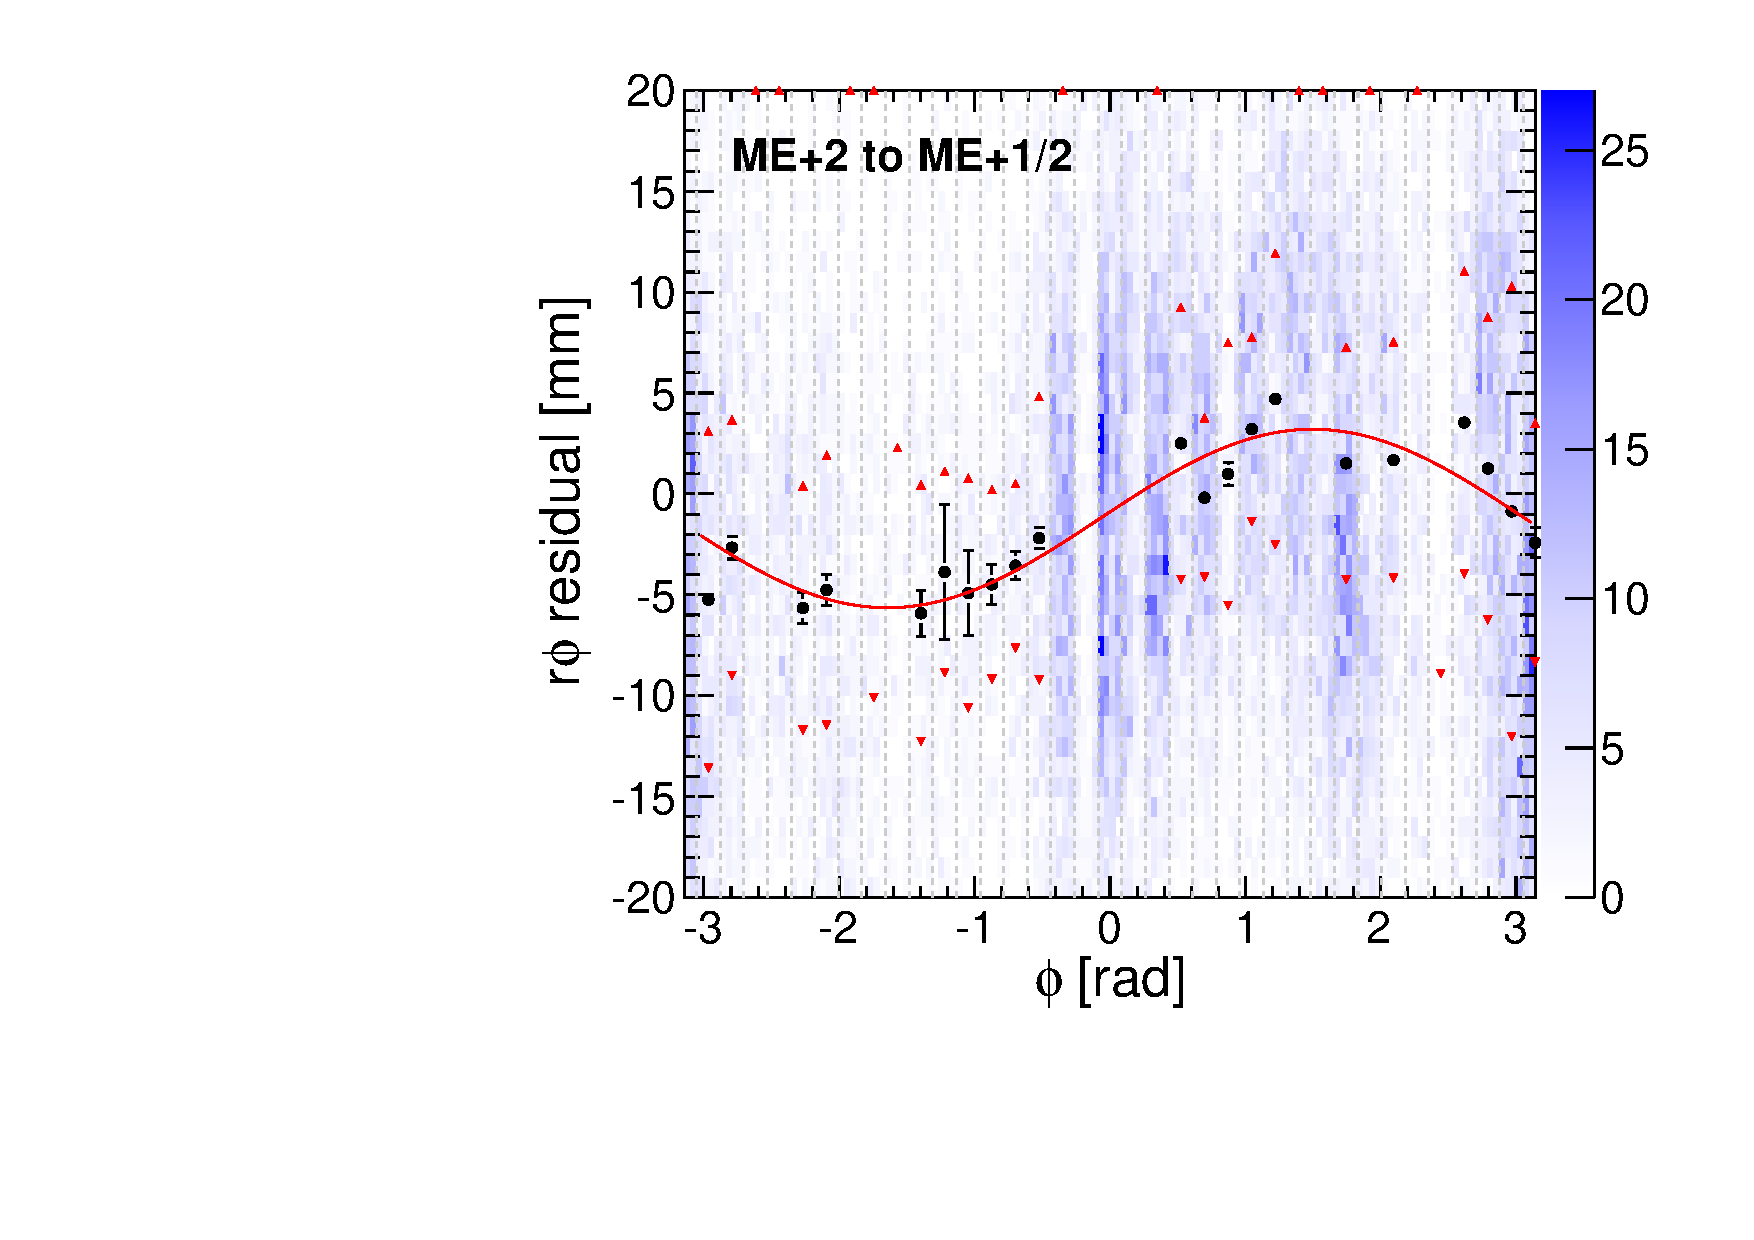
\includegraphics[width=0.4\linewidth]{BHCrossCheck_mep12_before.pdf}
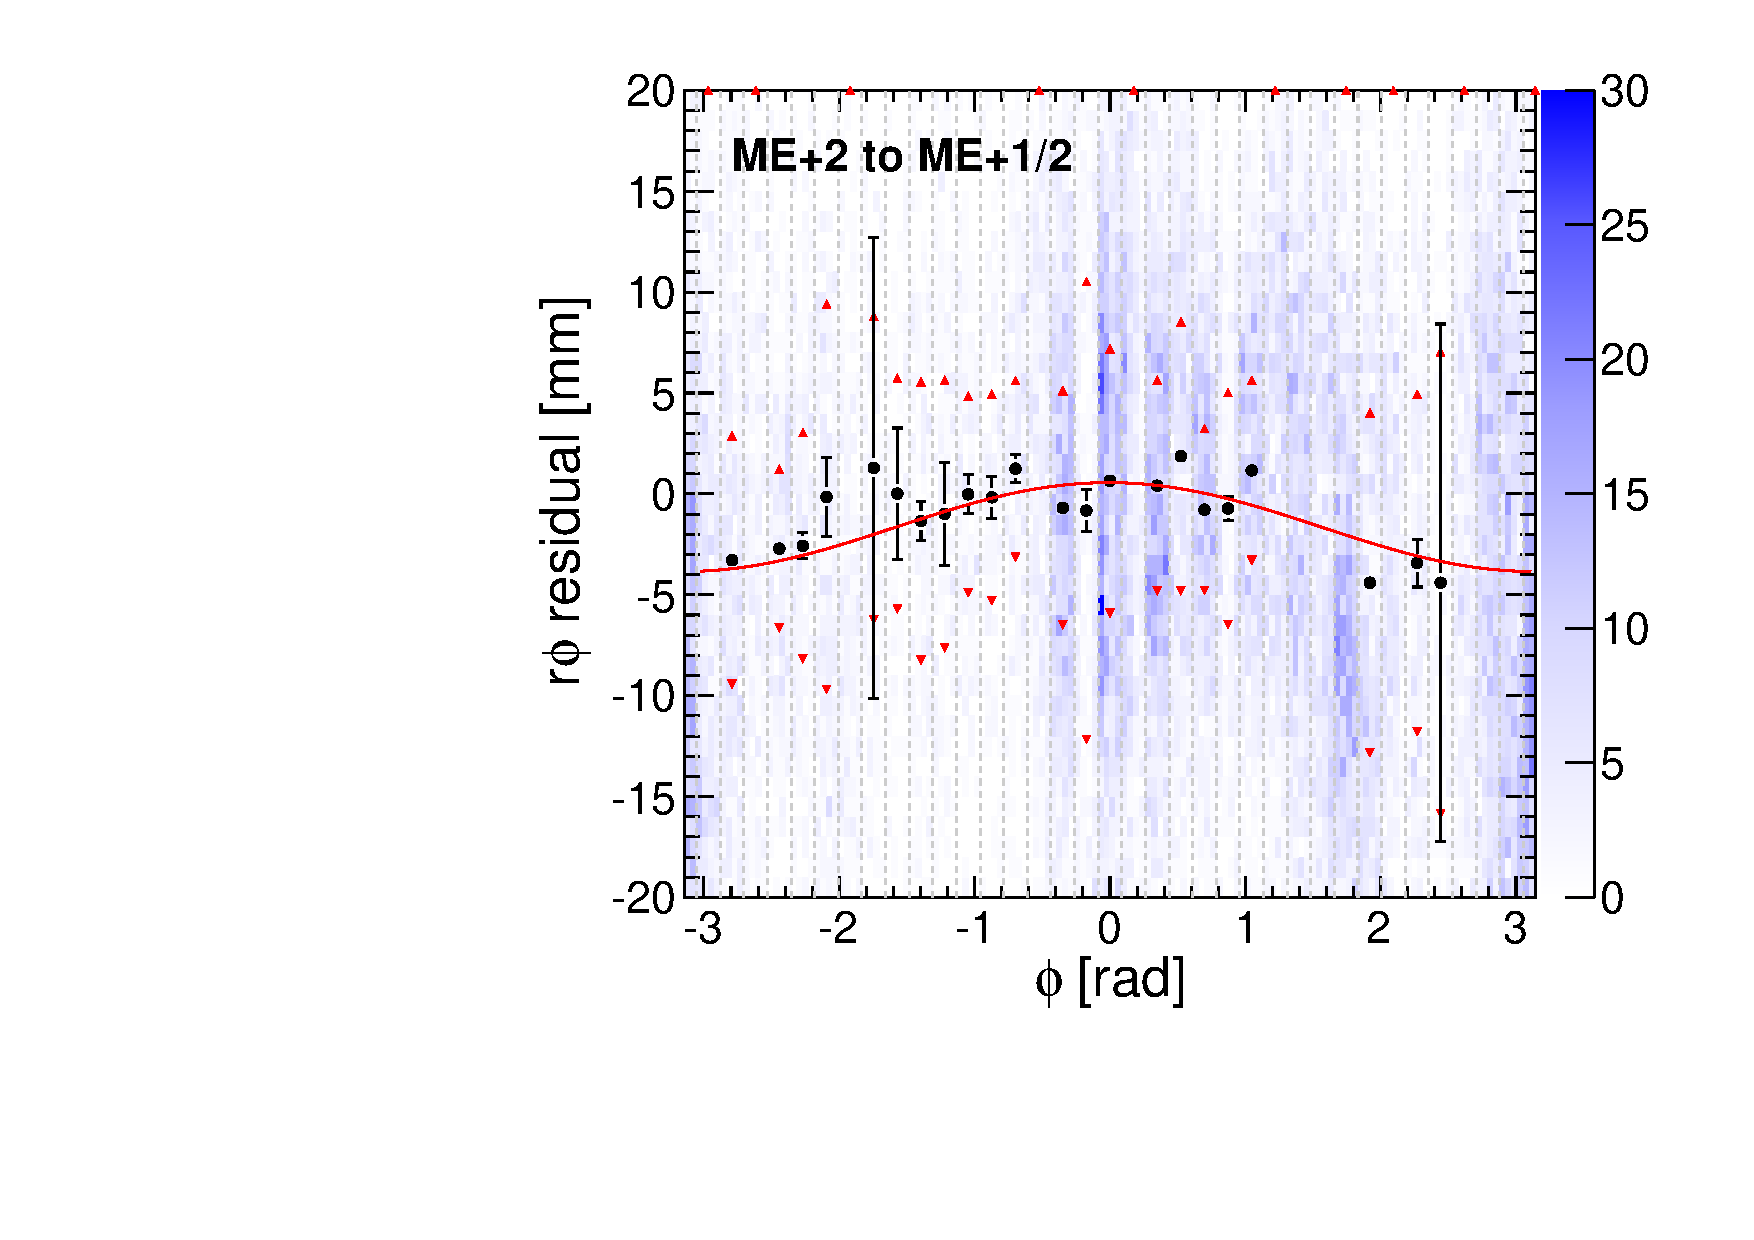
\includegraphics[width=0.4\linewidth]{BHCrossCheck_mep12_after.pdf}

\includegraphics[width=0.4\linewidth]{BHCrossCheck_mem12_before.pdf}
\includegraphics[width=0.4\linewidth]{BHCrossCheck_mem12_after.pdf}
\end{center}

\caption{Consistency of beam-halo segments linearly extrapolated from
  ME2 to ME1/2 with segments in ME1/2, before (left) and after
  (right) the independent tracker-to-muon ring alignment.  (See
  Fig.~\ref{fig:BHCrossCheck_me41} for additional explanation.)
  Differences between muons and antimuons (red triangles) are large
  because the radial magnetic field was not taken into account when
  propagating segments between stations.  (ME1/2 has poor beam-halo
  statistics.) \label{fig:BHCrossCheck_me12}}
\end{figure}

\begin{figure}
\begin{center}
\includegraphics[width=0.4\linewidth]{BHCrossCheck_mep13_before.pdf}
\includegraphics[width=0.4\linewidth]{BHCrossCheck_mep13_after.pdf}

\includegraphics[width=0.4\linewidth]{BHCrossCheck_mem13_before.pdf}
\includegraphics[width=0.4\linewidth]{BHCrossCheck_mem13_after.pdf}
\end{center}

\caption{Consistency of beam-halo segments linearly extrapolated from
  ME2/2 to ME1/3 with segments in ME1/3, before (left) and after
  (right) the independent tracker-to-muon ring alignment.  (See
  Fig.~\ref{fig:BHCrossCheck_me41} for additional explanation.)
  Differences between muons and antimuons (red triangles) are large
  because the radial magnetic field was not taken into account when
  propagating segments between stations.  (ME1/3 has poor beam-halo
  statistics.) \label{fig:BHCrossCheck_me13}}
\end{figure}

Figure~\ref{fig:BHCrossCheck_me41} is the most dramatic, showing that
even tracker-tracks propagated to the outermost muon station of CMS
yield alignment corrections accurate to a few hundred microns, when
observed with a completely independent method.  Comparisons closer to
the tracker are in less perfect agreement, but this is the region
where the beam-halo method is inaccurate due to larger magnetic
field corrections and lower statistics.  The tracker-to-muon
alignment, however, must be more accurate closer to the tracker,
because incorrectly-propagated tracks can only worsen with distance of
propagation.

The fit-values of the curve after alignment is presented in
Table~\ref{tab:second_systematics_table}.

\begin{table}
\caption{Fit results with statistical uncertainties for
  Figs.~\ref{fig:BHCrossCheck_me41}--\ref{fig:BHCrossCheck_me13},
  demonstrating the level of agreement between the tracker-to-ring
  method (Table~\ref{tab:results}) and the ring-to-ring
  method. \label{tab:second_systematics_table}}
\begin{center}
\renewcommand{\arraystretch}{1.2}
\begin{tabular}{c c c c c}
& $\delta_x$ (mm) & $\delta_y$ (mm) & $\delta_{\phi_z}$ (mrad) \\\hline
ME$+$3/1 $\to$ ME$+$4/1 & $-$0.029 $\pm$ 0.029 & $+$0.066 $\pm$ 0.023 & $-$0.140 $\pm$ 0.008 & Fig.~\ref{fig:BHCrossCheck_me41} \\
ME$+$2/2 $\to$ ME$+$3/2 & $-$0.420 $\pm$ 0.176 & $-$0.380 $\pm$ 0.166 & $-$0.060 $\pm$ 0.027 & Fig.~\ref{fig:BHCrossCheck_me32} \\
ME$+$2/1 $\to$ ME$+$3/1 & $+$0.126 $\pm$ 0.036 & $+$0.083 $\pm$ 0.027 & $-$0.104 $\pm$ 0.010 & Fig.~\ref{fig:BHCrossCheck_me31} \\
ME$+$2/2 $\to$ ME$+$1/3 & $-$2.204 $\pm$ 0.659 & $+$1.898 $\pm$ 0.579 & $+$0.005 $\pm$ 0.073 & Fig.~\ref{fig:BHCrossCheck_me13} \\
ME$+$2 $\to$ ME$+$1/2 & $-$0.012 $\pm$ 0.176 & $+$2.203 $\pm$ 0.153 & $-$0.511 $\pm$ 0.039 & Fig.~\ref{fig:BHCrossCheck_me12} \\
ME$+$2/1 $\to$ ME$+$1/1 & $+$0.621 $\pm$ 0.152 & $-$0.129 $\pm$ 0.117 & $+$0.153 $\pm$ 0.051 & Fig.~\ref{fig:BHCrossCheck_me11} \\\hline
ME$-$2/1 $\to$ ME$-$1/1 & $-$0.116 $\pm$ 0.137 & $-$0.469 $\pm$ 0.100 & $-$0.133 $\pm$ 0.044 & Fig.~\ref{fig:BHCrossCheck_me11} \\
ME$-$2 $\to$ ME$-$1/2 & $+$0.244 $\pm$ 0.214 & $+$0.733 $\pm$ 0.135 & $+$0.413 $\pm$ 0.048 & Fig.~\ref{fig:BHCrossCheck_me12} \\
ME$-$2/2 $\to$ ME$-$1/3 & $+$0.716 $\pm$ 0.710 & $+$0.998 $\pm$ 0.740 & $-$0.150 $\pm$ 0.090 & Fig.~\ref{fig:BHCrossCheck_me13} \\
ME$-$2/1 $\to$ ME$-$3/1 & $-$0.222 $\pm$ 0.038 & $-$0.246 $\pm$ 0.026 & $+$0.0786 $\pm$ 0.010 & Fig.~\ref{fig:BHCrossCheck_me31} \\
ME$-$2/2 $\to$ ME$-$3/2 & $+$0.114 $\pm$ 0.171 & $-$0.495 $\pm$ 0.193 & $-$0.172 $\pm$ 0.026 & Fig.~\ref{fig:BHCrossCheck_me32} \\
ME$-$3/1 $\to$ ME$-$4/1 & $+$0.008 $\pm$ 0.028 & $+$0.133 $\pm$ 0.021 & $+$0.142 $\pm$ 0.008 & Fig.~\ref{fig:BHCrossCheck_me41} \\\hline
\end{tabular}
\end{center}
\end{table}

\section{Stability of internal chamber alignment}
\label{sec:stability}

In this last section, we revisit the internal chamber alignment in
light of the new ring positions and what we learned from the
collisions muons that produced it.  The internal ring alignment
procedure using beam-halo overlaps is described in detail in the
Oct.~29 HyperNews paper.

The first question we should ask is whether the two alignments can
truly be factorized: if we re-align the internal geometry starting
from the new ring positions, do we obtain the same relative positions?
This can be quantified by comparing the chamber positions after the
tracker-to-ring alignment but before re-aligning the chambers with
beam-halo overlaps.  These differences are histogrammed in
Fig.~\ref{fig:effectofdisk}.  Only in ME$\pm$1/2 are the differences
non-negligible (RMS of 0.8~mm), and these are the only two rings that
have antipodal photogrammetry constraints.  (The only other ring with
more than one photogrammetry constraint is ME$+$2/2, but these are
only 4 chambers apart.)  This is relevant because the photogrammetry
applies $r\phi$ position constraints relative to a ring center that is
not equal to the ring center derived from the tracker-to-ring
alignment.  The photogrammetry coordinate frame is allowed to float,
but in only one dimension, $\phi$, though the ring origin was moved in
two dimensions, $x$ and $y$.  Thus, the photogrammetry's coordinate
system can pull chambers in the ring if it applies two or more
constraints with a significant distance between them.  This effect can
be seen clearly by plotting these same chamber corrections as a
function of chamber number ($\phi$) in
Fig.~\ref{fig:effectofdisk_ring}: the largest deviation occurs at the
constraints with all other chambers interpolating in between.

\begin{figure}
\includegraphics[width=0.24\linewidth]{effectofdisk_me11.pdf}
\includegraphics[width=0.24\linewidth]{effectofdisk_me12.pdf}
\includegraphics[width=0.24\linewidth]{effectofdisk_inner234.pdf}
\includegraphics[width=0.24\linewidth]{effectofdisk_outer.pdf}

\caption{Differences in chamber $r\phi$ positions before and after
  re-alignment with the new ring positions.  Only ME$\pm$1/2 are
  significantly affected, and these two rings are the only ones with
  antipodal photogrammetry constraints. \label{fig:effectofdisk}}
\end{figure}

\begin{figure}
\includegraphics[width=0.5\linewidth]{effectofdisk_ring_mep12.pdf}
\includegraphics[width=0.5\linewidth]{effectofdisk_ring_mem12.pdf}

\caption{Differences in ME$\pm$1/2 $r\phi$ chamber positions
  (Fig.~\ref{fig:effectofdisk}) in greater detail, showing the
  locations of the missing beam-halo data/photogrammetry constraints.
  The disks are being distorted by the photogrammetry's coordinate
  system (a ring position that is different from what was determined
  by the tracker-to-ring alignment). \label{fig:effectofdisk_ring}}
\end{figure}

To avoid this, we can simply apply no more than one photogrammetry
constraint per ring.  This has the advantage that the photogrammetry
effectively becomes a simple two-chamber constraint, since it
specifies the locations of neighboring chambers $A$ and $B$ relative
to an origin $\mathcal{O}$ which is allowed to float: the only forced
condition is for $A-B$ to have a given value.  It has the disadvantage
that the network of alignables becomes an unclosed loop: uncertainties
grow with distance from the constraint.
Figure~\ref{fig:effectofdiskOnlyOne_ring} shows what happens to
ME$\pm$1/2 when only one of the two photogrammetry constraints is
required: chambers connected purely by beam-halo measurements are
shifted as coherent groups.  By applying this looser photogrammetry
constraint, the internal ring alignments can be made independent of
changes in the overall ring position.

\begin{figure}
\includegraphics[width=0.5\linewidth]{effectofdiskOnlyOne_ring_mep12.pdf}
\includegraphics[width=0.5\linewidth]{effectofdiskOnlyOne_ring_mem12.pdf}

\caption{Differences in ME$\pm$1/2 $r\phi$ chamber positions with only
  one photogrammetry constraint per ring: compare to
  Fig.~\ref{fig:effectofdisk_ring}.  A constraint was applied in
  ME$+$1/2 chambers 14--16 and ME$-$1/2 chambers
  33--34. \label{fig:effectofdiskOnlyOne_ring}}
\end{figure}

During the tracker-to-ring procedure, large internal misalignments
were observed in ME1/1, which was not unexpected, since ME1/1 rings
are missing beam-halo data at several points without photogrammetry to
fill the gaps.  To use this information in a way that minimally
depends on tracker-to-muon propagations, one can align the chambers
bordering the missing beam-halo data by hand from the collisions data
and feed these into the beam-halo overlaps alignment as new
constraints.  Figure~\ref{fig:byhand} shows the ME1/1 residuals
distribution as seen by collisions muons with green boxes highlighting
the 12 chambers aligned by hand.  Figures~\ref{fig:newconstraints} and
\ref{fig:newconstraintsPhiZ} show the effect that these new
constraints have on the beam-halo alignment of ME1/1.

\begin{figure}
\includegraphics[width=0.5\linewidth]{byhand_mep11.pdf}
\includegraphics[width=0.5\linewidth]{byhand_mem11.pdf}

\caption{Alignment of 12 chambers by hand using the collisions data.
  The purpose of this is to provide constraints at key points for the
  beam-halo overlaps alignment. \label{fig:byhand}}
\end{figure}


\begin{figure}
\includegraphics[width=0.5\linewidth]{newconstraintsPlus.pdf}
\includegraphics[width=0.5\linewidth]{newconstraintsMinus.pdf}

\caption{Changes in the beam-halo overlaps alignment caused by the 12
  new constraints in ME1/1 ($r\phi$).  Since these points had
  previously been unconstrained by any data, these changes are likely
  an improvement. \label{fig:newconstraints}}
\end{figure}

\begin{figure}
\includegraphics[width=0.5\linewidth]{newconstraintsPlusPhiZ.pdf}
\includegraphics[width=0.5\linewidth]{newconstraintsMinusPhiZ.pdf}

\caption{Changes in the beam-halo overlaps alignment caused by the 12
  new constraints in ME1/1 ($\phi_z$).  Since these points had
  previously been unconstrained by any data, these changes are likely
  an improvement. \label{fig:newconstraintsPhiZ}}
\end{figure}

In summary, we have made two minor modifications to the beam-halo
overlaps alignment procedure, inspired by the collisions residuals:
\begin{itemize}
\item now only one group of nearby chambers per ring is constrained by
  photogrammetry, to avoid imposing the photogrammetry's coordinate
  frame on the ring geometry;
\item now the ME1/1 beam-halo fit is constrained at six points with
  measurements derived from collisions residuals.
\end{itemize}
A list of constrained chambers is given in Table~\ref{tab:pgholes}.
This is the internal ring geometry we propose for sign-off.

\begin{table}
\caption{Photogrammetry and collisions data used to constrain final
  beam-halo overlaps alignment.  Only one point in each ring is
  constrained by photogrammetry, and constraints from collisions data
  are expressed in the tracker's coordinate system. \label{tab:pgholes}}
\begin{center}
\begin{tabular}{r l}
Photogrammetry & ME$+$4/1/14 and ME$+$4/1/15 \\
constraints & ME$+$3/2/18 and ME$+$3/2/19 \\
& ME$+$2/2/19 and ME$+$2/2/20 \\
& ME$+$2/1/01 and ME$+$2/1/02 \\
& ME$+$1/2/14, ME$+$1/2/15, and ME$+$1/2/16 \\
& ME$-$1/2/33 and ME$-$1/2/34 \\
& ME$-$2/1/06 and ME$-$2/1/07 \\
& ME$-$2/2/02, ME$-$2/2/03, and ME$-$2/2/04 \\
& \\
Constraints from & ME$+$1/1/01 and ME$+$1/1/03 \\
TrackerMuon residuals & ME$+$1/1/19 and ME$+$1/1/21 \\
& ME$+$1/1/30 and ME$+$1/1/31 \\
& ME$-$1/1/14 and ME$-$1/1/16 \\
& ME$-$1/1/33 and ME$-$1/1/35 \\
& ME$-$1/1/30 and ME$-$1/1/31 \\
\end{tabular}
\end{center}
\end{table}

\section{Conclusions: recommended endcap constants}

In summary, we have aligned the CSC rings relative to the tracker,
independently confirmed their positions using beam-halo muons that
cross multiple stations, and have updated the internal alignment of
rings in light of observations from the collisions residuals.  The
updated internal ring alignment is final, to be submitted for
approval.  The alignment of the rings will need to be repeated using
the latest tracker description and cross-alignment, but using exactly
the methods described in Sec.~\ref{sec:trackertorings}.

\subsection{Provenance of set of constants}

The internally aligned CSC geometry can be found here:

{\tt \small /afs/cern.ch/user/p/pivarski/public/NOV05\_PG-HW-phiy-BHPGholes-rings2-BHPGholes2.db}

\noindent The following procedures have been applied to this set of constants, in the following order:

\begin{enumerate}
\item Photogrammetry: local $x$, $y$, $z$, $\phi_x$, $\phi_z$;
\item SLM lines for disk displacement and bending due to magnetic field: local $z$, $\phi_x$ (replacing PG);
\item ``Missing angle measurement'' from collisions relative to the
  tracker: local $\phi_y$ (see Jim's talk at the Oct.~8 Muon Alignment
  meeting\footnote{\url{http://indico.cern.ch/conferenceDisplay.py?confId=109787}});
\item Beam-halo alignment of chambers relative to rings, with PG
  constraining only the gaps in the beam-halo data (no PG constraint
  in ME1/1): $r\phi$ and $\phi_z$ (replacing PG), see the Oct.~29
  HyperNews paper;
\item Ring alignment using collisions: global $x$, $y$, $\phi_z$ of
  rings, keeping internal chamber structure intact
  (Sec.~\ref{sec:trackertorings} of this note);
\item Beam-halo re-alignment of chambers relative to rings, with only
  one PG constraint per ring and with ME1/1 constraints derived from
  collisions (Sec.~\ref{sec:stability} of this note).
\end{enumerate}

\subsection{Well-defined methods to repeat with the latest tracker and cross-alignments}

Now that these procedures have been defined, they must be repeated
with the new tracker alignment and tracker/muon system
cross-alignment.  The following will be performed with the latest
tracker description (calibration and alignment) and cross-alignment
results (GlobalAlignmentRcd):
\begin{enumerate}
\item Re-run the tracker-to-ring alignment exactly as it was done
  here, updating global ring parameters only.
\item Verify that the updates are smaller than 1~mm, 1~mrad or are
  consistent with a global translation/rotation.
\item Submit the resulting geometry for approval before Nov.~12, but
  likely much sooner.
\item When approved, upload it to the database and notify the Muon POG for testing.
\end{enumerate}

\end{document}
